\documentclass[11pt]{article}

\usepackage{../style/paper_theme_dobbins}
\graphicspath{{../figures/}}

\author[1]{Iordanis Pantzartzis}
\affil[1]{Universität Konstanz, 01/1001158}
\matric{01/1001158}
\seminar{Comparative politics and public policy}
\supervisor{Adj. Prof. Dr. Michael Dobbins}
\semester{Winter semester 2024/2025}
\submitdate{15. February 2025}
\title{U.S. healthcare reform and policy feedback: Some fancy subtitle}
\abs{Placeholder}
\seminartype{M.A. Seminar}
\keywords{healthcare, policy feedback}
%------------------------------------------------------

\begin{document}

% {\small

\newgeometry{includehead, includefoot, left=1.75cm, right=2.25cm, top=4.58cm, bottom=1.17cm, headheight=0cm, footskip=1.17cm, headsep=0cm}

\thispagestyle{page1}


\begin{tikzpicture}[remember picture,overlay]
    \node[anchor=north east,inner sep=0pt] at (current page.north east) {
\includegraphics[scale=1]{_uni_logo.pdf}};
    \draw [line width=1pt, color =kon9] ($(current page.north west) + (0.8cm,-10.5cm)$) -- ++(0.5cm,0);
    \draw [line width=1pt, color =kon9] ($(current page.north west) + (0.8cm,-14.85cm)$) -- ++(0.5cm,0);
 \end{tikzpicture}


\setstretch{1.1}
\setlength{\parindent}{0cm}
\myhelvetica

{
    \raggedleft
    \small

    \textbf{\normalsize\ul{Department of Politics and Public Administration}}

    \setstretch{1}
    \scriptsize
    \vspace{0.4cm}

    Universitätsstraße 10

    D-78457 Konstanz

    \vspace{0.2cm}

    www.polver.uni-konstanz.de

}

\vspace{0.25cm}
\begingroup
{\large{\textbf{\ul{Declaration of Authorship}}}}

\raggedright
\vspace{0.25cm}

\begin{justify}
    It is considered plagiarism if text or ideas from other works (books, journals, the Internet, etc.) are adopted or translated without proper citation in your scientific paper and thus falsely passed off as your own intellectual achievement.
\end{justify}


\vspace{0.5cm}

\begin{tblr}{
    width=\linewidth,
    rows={ht=0.7cm},
    colspec={X[2]X[30]X[18]},
    cells= {
            valign=f,
            halign=left, 
            },
    cell{1}{2-3}={bg=black!10, font=\scriptsize},
    rowsep=0cm,
    hline{1-Z}={2-Z}{solid},
    vline{3,4}={},
}
    I &something & something\\
\end{tblr}

\vspace{0.2cm}

hereby declare that the attached paper for the following class

\vspace{-0.3cm}

\begin{center}
    \begin{tblr}{
        width=0.975\linewidth,
        rows={ht=1.5cm, },
        colspec={X},
        cells= {
            valign=h,
            halign=left,
            bg=black!10,
            font=\scriptsize,
            },
        rowsep=0cm,
        hlines={},
        vlines={},
    }
    something\\
    \end{tblr}
\end{center}


\vspace{-0.1cm}

on the following topic

\vspace{-0.3cm}

\begin{center}
    \begin{tblr}{
        width=0.975\linewidth,
        rows={ht=1.5cm, },
        colspec={X},
        cells= {
            valign=h, 
            halign=left, 
            bg=black!10,
            font=\scriptsize,
            },
        rowsep=0cm,
        hlines={},
        vlines={},
    }
    something\\
    \end{tblr}
\end{center}


\vspace{0.3cm}


is the result of my own, independent work. I have not used any aids or sources other than those I have referenced in the document. For contributions and quotations from the works of other people (whether distributed electronically or in hardcopy), I have identified each of them with a reference to the source or the secondary literature. Failure to do so constitutes plagiarism. I will also submit the term paper electronically to the lecturer.\\

\vspace{\baselineskip}

Furthermore, I declare that the above mentioned work has not been
otherwise submitted as a term paper.\\

\vspace{\baselineskip}

Regarding the use of generative AI tools, I met the guidelines of the
lecturer and clarified them in case of doubt.


\def\LayoutCheckField#1#2{% label, field
  #2 #1%
}

\begin{itemize}[labelwidth=0.65cm,align=parleft]
    \item[\mbox{\begin{Form}\CheckBox[height=0.2cm, width=0.2cm]{}\end{Form}}] I have used generative AI tools as an aid within the limits allowed by the lecturer. I understand that I am solely responsible for the accuracy of the content of the AI-generated text passages, as well as for referencing other people\textquotesingle s wording and ideas in accordance with the principles of good scientific practice. In the case of an adoption of AI-generated passages that go beyond purely formal, stylistic corrections, I have marked them and, in addition to the AI tool used, I have indicated the prompts I entered.
    
        
    \item[\mbox{\begin{Form}\CheckBox[height=0.2cm, width=0.2cm]{}\end{Form}}]I did not use any generative AI tools as aids.
\end{itemize}
\endgroup


\newpage
% %------------------------------------------------------
\thispagestyle{page2}


\begin{tikzpicture}[remember picture,overlay]
    \node[anchor=north east,inner sep=0pt] at (current page.north east) {
\includegraphics[scale=1]{_uni_logo.pdf}};
    \draw [line width=1pt, color =kon9] ($(current page.north west) + (0.8cm,-10.5cm)$) -- ++(0.5cm,0);
    \draw [line width=1pt, color =kon9] ($(current page.north west) + (0.8cm,-14.85cm)$) -- ++(0.5cm,0);
 \end{tikzpicture}

I am aware of the following:

\begin{itemize}[label=\color{kon4}--, leftmargin=1.45cm, labelsep=0.45cm]
\item I am guilty of plagiarism if, contrary to the requirements set out above, I use the work of others in my thesis without acknowledging the precise source. This would be to lay claim to an achievement that is not my own.

\item If a candidate intentionally violates the University of Konstanz's Statutes to Ensure Good Scientific Practice when composing his/her thesis, it will be, in all probability, judged as an attempt at cheating (plagiarism). This means that the thesis will be graded \enquote{nicht ausreichend/fail} (5,0), placed on record in the student's examination file, and put before the Examination Board (StPA).

\item In repeated or particularly serious cases, the StPA may decide to exclude the candidate from further performance assessments, resulting in a complete loss of right to take any further examinations in this study programme.

\item The legal basis for this is laid down in the applicable examination regulations for the study programme in question.
\end{itemize}

I have taken note of these guidelines regarding plagiarism.

\vspace{0.75cm}

\begin{minipage}{0.3\textwidth}
    % \renewcommand{\arraystretch}{3.5}
    % \begin{tabulary}{\textwidth}{|X|}
    %     \hline
    %     \\
    %     \hline
    % \end{tabulary}

    % \vspace{0.1cm}
    \begin{tblr}{
        width=\linewidth,
        rows={ht=2cm, valign=b},
        colspec={Q[f, \linewidth]},
        cells= {halign=left},
        rowsep=0cm,
        hlines={},
        vlines={},
    }
   Konstanz, \@submitdate\\
    \end{tblr}

    \vspace{0.1cm}

    Place, date
\end{minipage}\begin{minipage}{0.1\textwidth}
     \phantom{a}
\end{minipage}\begin{minipage}{0.6\textwidth}
    \begin{tblr}{
        width=\linewidth,
        rows={ht=2cm, valign=b},
        colspec={X},
        cells= {halign=left},
        rowsep=0cm,
        hlines={},
        vlines={},
    }
   
\includegraphics[height=1.9cm]{signature_iordanis2.pdf}\\
    \end{tblr}

    \vspace{0.1cm}

    \raggedleft Student's signature
\end{minipage}
}
\newpage
\restoregeometry

% \restoregeometry

\maketitle

%------------------------------------------------------
% \restoregeometry
% \thispagestyle{fancy}
\section*{Introduction}

When (then candidate) Donald Trump was asked in his, first and only, presidential debate with Democratic opponent Kamala Harris what his plans for healthcare reform were, his response that he had \enquote{concepts of plan} \parencite[][]{Trump2024} rekindled some discourse as to the future of American healthcare and potential reforms in that sector. Ever since it was passed, Republican lawmakers, in conjunction with candidate and president Trump, have at times alternately advocated for -- and attempted -- repealing President Barack Obama's signature healthcare reform, the Patient Protection and Affordable Care Act (abbreviated as ACA, commonly also referred to as \enquote{Obamacare}), outright, or making major modifications to the law \parencite[][]{Armour2024}. However, neither a repeal or a major modification ever came to pass, despite Republicans gaining control of the White House and both Houses of Congress following the 2016 general election \parencite[][]{FEC2016}. Three Republican Senators voted to \textit{not} repeal Obamacare, Senator John McCain, as was highly publicized at the time, voting no via thumbs-down on the Senate floor, less than two days after receiving surgery for brain cancer \parencite[][]{Davis2016}. Beyond any individual-level intuitions for this specific legislative outcome, this suggest the question \textit{why were Republicans unable to repeal or reform the ACA?} One explanation might be public response -- in the time since its passage, the ACA's popularity has somewhat transformed, from being viewed rather controversially in the beginning, to now (early 2025) enjoying its largest net positive favorability ever (see \hyperref[fig:aca_fav]{Figure 1}):\\

% \begin{figure}[H]
%     \caption{Affordable Care Act favorability 2010-2025.}
%     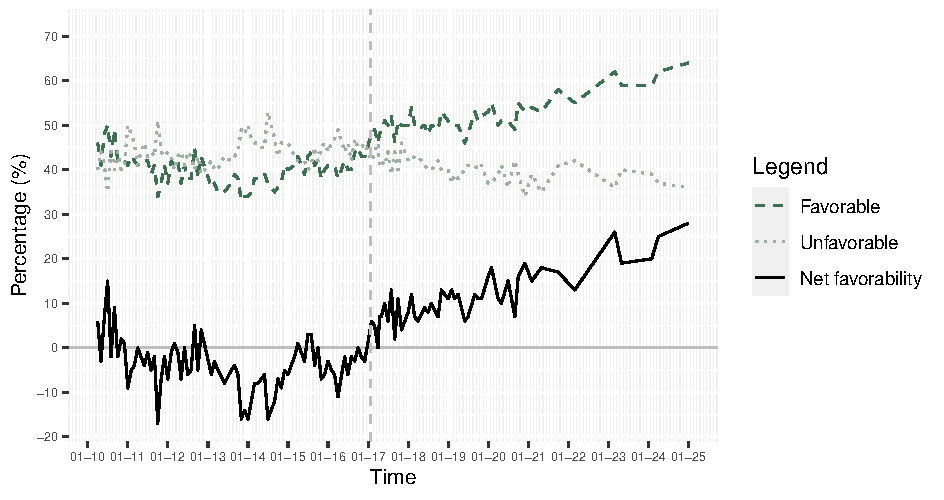
\includegraphics{_aca_fav.pdf}
%     \label{fig:aca_fav}
%     \caption*{\textit{Note}: Data source \textcite[][]{KFF1}}
% \end{figure}

\begin{figure}[H]
  \sffamily
  \caption{ACA favorability (2010--22023)}
  % Created by tikzDevice version 0.12.6 on 2025-02-04 18:07:37
% !TEX encoding = UTF-8 Unicode
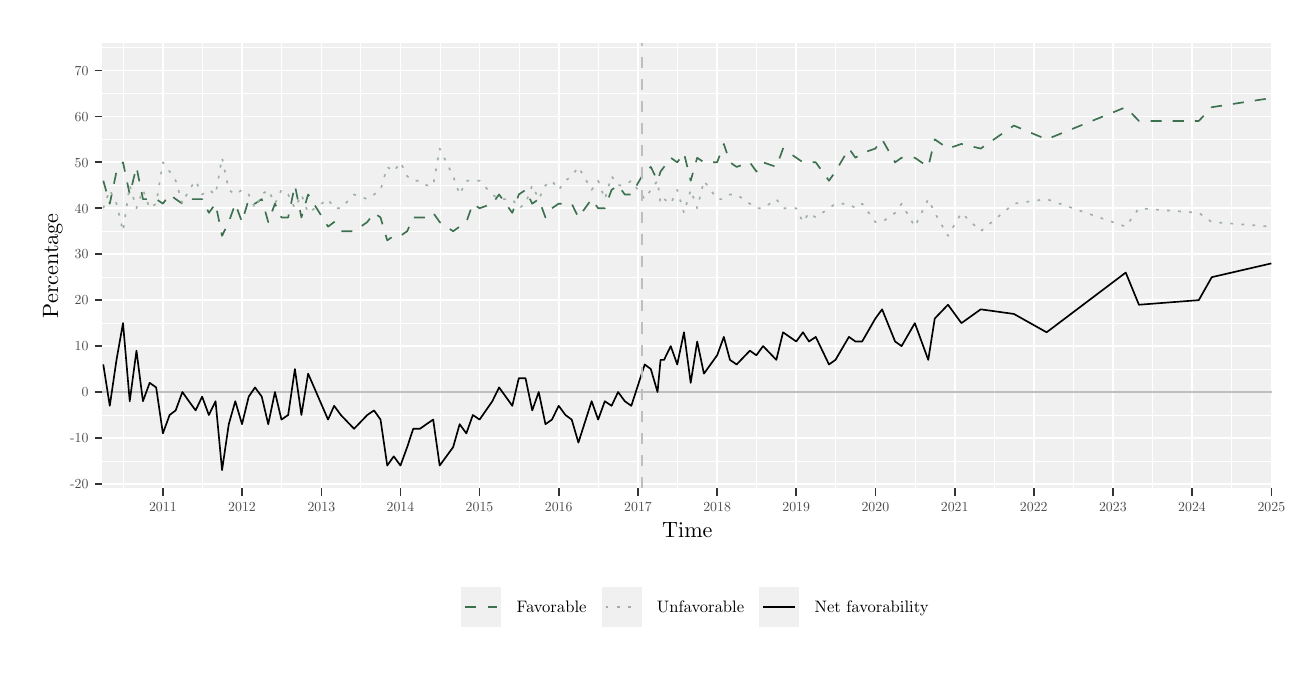
\begin{tikzpicture}[x=1pt,y=1pt]
\definecolor{fillColor}{RGB}{255,255,255}
\path[use as bounding box,fill=fillColor,fill opacity=0.00] (0,0) rectangle (455.30,227.65);
\begin{scope}
\path[clip] (  0.00,  0.00) rectangle (455.30,227.65);
\definecolor{drawColor}{RGB}{255,255,255}
\definecolor{fillColor}{RGB}{255,255,255}

\path[draw=drawColor,line width= 0.6pt,line join=round,line cap=round,fill=fillColor] (  0.00,  0.00) rectangle (455.30,227.65);
\end{scope}
\begin{scope}
\path[clip] ( 26.93, 61.13) rectangle (449.80,222.15);
\definecolor{fillColor}{gray}{0.94}

\path[fill=fillColor] ( 26.93, 61.13) rectangle (449.80,222.15);
\definecolor{drawColor}{RGB}{255,255,255}

\path[draw=drawColor,line width= 0.3pt,line join=round] ( 26.93, 71.09) --
	(449.80, 71.09);

\path[draw=drawColor,line width= 0.3pt,line join=round] ( 26.93, 87.69) --
	(449.80, 87.69);

\path[draw=drawColor,line width= 0.3pt,line join=round] ( 26.93,104.29) --
	(449.80,104.29);

\path[draw=drawColor,line width= 0.3pt,line join=round] ( 26.93,120.89) --
	(449.80,120.89);

\path[draw=drawColor,line width= 0.3pt,line join=round] ( 26.93,137.49) --
	(449.80,137.49);

\path[draw=drawColor,line width= 0.3pt,line join=round] ( 26.93,154.09) --
	(449.80,154.09);

\path[draw=drawColor,line width= 0.3pt,line join=round] ( 26.93,170.69) --
	(449.80,170.69);

\path[draw=drawColor,line width= 0.3pt,line join=round] ( 26.93,187.29) --
	(449.80,187.29);

\path[draw=drawColor,line width= 0.3pt,line join=round] ( 26.93,203.89) --
	(449.80,203.89);

\path[draw=drawColor,line width= 0.3pt,line join=round] ( 26.93,220.49) --
	(449.80,220.49);

\path[draw=drawColor,line width= 0.3pt,line join=round] ( 34.57, 61.13) --
	( 34.57,222.15);

\path[draw=drawColor,line width= 0.3pt,line join=round] ( 63.15, 61.13) --
	( 63.15,222.15);

\path[draw=drawColor,line width= 0.3pt,line join=round] ( 91.78, 61.13) --
	( 91.78,222.15);

\path[draw=drawColor,line width= 0.3pt,line join=round] (120.41, 61.13) --
	(120.41,222.15);

\path[draw=drawColor,line width= 0.3pt,line join=round] (149.00, 61.13) --
	(149.00,222.15);

\path[draw=drawColor,line width= 0.3pt,line join=round] (177.59, 61.13) --
	(177.59,222.15);

\path[draw=drawColor,line width= 0.3pt,line join=round] (206.21, 61.13) --
	(206.21,222.15);

\path[draw=drawColor,line width= 0.3pt,line join=round] (234.84, 61.13) --
	(234.84,222.15);

\path[draw=drawColor,line width= 0.3pt,line join=round] (263.43, 61.13) --
	(263.43,222.15);

\path[draw=drawColor,line width= 0.3pt,line join=round] (292.02, 61.13) --
	(292.02,222.15);

\path[draw=drawColor,line width= 0.3pt,line join=round] (320.64, 61.13) --
	(320.64,222.15);

\path[draw=drawColor,line width= 0.3pt,line join=round] (349.27, 61.13) --
	(349.27,222.15);

\path[draw=drawColor,line width= 0.3pt,line join=round] (377.86, 61.13) --
	(377.86,222.15);

\path[draw=drawColor,line width= 0.3pt,line join=round] (406.45, 61.13) --
	(406.45,222.15);

\path[draw=drawColor,line width= 0.3pt,line join=round] (435.08, 61.13) --
	(435.08,222.15);

\path[draw=drawColor,line width= 0.6pt,line join=round] ( 26.93, 62.79) --
	(449.80, 62.79);

\path[draw=drawColor,line width= 0.6pt,line join=round] ( 26.93, 79.39) --
	(449.80, 79.39);

\path[draw=drawColor,line width= 0.6pt,line join=round] ( 26.93, 95.99) --
	(449.80, 95.99);

\path[draw=drawColor,line width= 0.6pt,line join=round] ( 26.93,112.59) --
	(449.80,112.59);

\path[draw=drawColor,line width= 0.6pt,line join=round] ( 26.93,129.19) --
	(449.80,129.19);

\path[draw=drawColor,line width= 0.6pt,line join=round] ( 26.93,145.79) --
	(449.80,145.79);

\path[draw=drawColor,line width= 0.6pt,line join=round] ( 26.93,162.39) --
	(449.80,162.39);

\path[draw=drawColor,line width= 0.6pt,line join=round] ( 26.93,178.99) --
	(449.80,178.99);

\path[draw=drawColor,line width= 0.6pt,line join=round] ( 26.93,195.59) --
	(449.80,195.59);

\path[draw=drawColor,line width= 0.6pt,line join=round] ( 26.93,212.19) --
	(449.80,212.19);

\path[draw=drawColor,line width= 0.6pt,line join=round] ( 48.86, 61.13) --
	( 48.86,222.15);

\path[draw=drawColor,line width= 0.6pt,line join=round] ( 77.45, 61.13) --
	( 77.45,222.15);

\path[draw=drawColor,line width= 0.6pt,line join=round] (106.12, 61.13) --
	(106.12,222.15);

\path[draw=drawColor,line width= 0.6pt,line join=round] (134.70, 61.13) --
	(134.70,222.15);

\path[draw=drawColor,line width= 0.6pt,line join=round] (163.29, 61.13) --
	(163.29,222.15);

\path[draw=drawColor,line width= 0.6pt,line join=round] (191.88, 61.13) --
	(191.88,222.15);

\path[draw=drawColor,line width= 0.6pt,line join=round] (220.55, 61.13) --
	(220.55,222.15);

\path[draw=drawColor,line width= 0.6pt,line join=round] (249.14, 61.13) --
	(249.14,222.15);

\path[draw=drawColor,line width= 0.6pt,line join=round] (277.72, 61.13) --
	(277.72,222.15);

\path[draw=drawColor,line width= 0.6pt,line join=round] (306.31, 61.13) --
	(306.31,222.15);

\path[draw=drawColor,line width= 0.6pt,line join=round] (334.98, 61.13) --
	(334.98,222.15);

\path[draw=drawColor,line width= 0.6pt,line join=round] (363.57, 61.13) --
	(363.57,222.15);

\path[draw=drawColor,line width= 0.6pt,line join=round] (392.15, 61.13) --
	(392.15,222.15);

\path[draw=drawColor,line width= 0.6pt,line join=round] (420.74, 61.13) --
	(420.74,222.15);

\path[draw=drawColor,line width= 0.6pt,line join=round] (449.41, 61.13) --
	(449.41,222.15);
\definecolor{drawColor}{RGB}{190,190,190}

\path[draw=drawColor,line width= 0.6pt,line join=round] ( 26.93, 95.99) -- (449.80, 95.99);
\definecolor{drawColor}{RGB}{60,113,79}

\path[draw=drawColor,line width= 0.6pt,dash pattern=on 4pt off 4pt ,line join=round] ( 27.32,172.35) --
	( 29.67,164.05) --
	( 32.10,175.67) --
	( 34.45,178.99) --
	( 36.88,167.37) --
	( 39.31,177.33) --
	( 41.65,165.71) --
	( 44.08,165.71) --
	( 46.43,165.71) --
	( 48.86,164.05) --
	( 51.29,167.37) --
	( 53.48,165.71) --
	( 55.91,164.05) --
	( 58.26,165.71) --
	( 60.69,165.71) --
	( 63.04,165.71) --
	( 65.47,160.73) --
	( 67.89,164.05) --
	( 70.24,152.43) --
	( 72.67,157.41) --
	( 75.02,164.05) --
	( 77.45,157.41) --
	( 79.88,165.71) --
	( 82.15,164.05) --
	( 84.58,165.71) --
	( 86.93,157.41) --
	( 89.35,164.05) --
	( 91.70,159.07) --
	( 94.13,159.07) --
	( 96.56,170.69) --
	( 98.91,159.07) --
	(101.34,167.37) --
	(108.54,155.75) --
	(110.74,157.41) --
	(113.16,154.09) --
	(117.94,154.09) --
	(122.72,157.41) --
	(125.15,160.73) --
	(127.50,159.07) --
	(129.93,150.77) --
	(132.28,152.43) --
	(134.70,152.43) --
	(137.13,154.09) --
	(139.32,159.07) --
	(141.75,159.07) --
	(144.10,159.07) --
	(146.53,160.73) --
	(148.88,157.41) --
	(153.74,154.09) --
	(156.09,155.75) --
	(158.51,157.41) --
	(160.86,164.05) --
	(163.29,162.39) --
	(167.91,164.05) --
	(170.34,167.37) --
	(175.12,160.73) --
	(177.47,167.37) --
	(179.90,169.03) --
	(182.32,164.05) --
	(184.67,165.71) --
	(187.10,159.07) --
	(189.45,162.39) --
	(191.88,164.05) --
	(194.31,164.05) --
	(196.58,164.05) --
	(199.01,159.07) --
	(203.79,165.71) --
	(206.14,162.39) --
	(208.56,162.39) --
	(210.99,169.03) --
	(213.34,170.69) --
	(215.77,167.37) --
	(218.12,167.37) --
	(222.97,175.67) --
	(225.17,177.33) --
	(227.60,172.35) --
	(228.69,175.67) --
	(229.95,177.33) --
	(232.37,180.65) --
	(234.72,178.99) --
	(237.15,182.31) --
	(239.58,172.35) --
	(241.93,180.65) --
	(244.36,178.99) --
	(249.14,178.99) --
	(251.56,185.63) --
	(253.76,178.99) --
	(256.18,177.33) --
	(260.96,178.99) --
	(263.31,175.67) --
	(265.74,178.99) --
	(270.52,177.33) --
	(272.95,183.97) --
	(277.72,180.65) --
	(280.15,178.99) --
	(282.34,178.99) --
	(284.77,178.99) --
	(289.55,172.35) --
	(291.90,175.67) --
	(296.76,183.97) --
	(299.11,180.65) --
	(301.53,182.31) --
	(306.31,183.97) --
	(308.74,187.29) --
	(313.44,178.99) --
	(315.79,180.65) --
	(320.57,180.65) --
	(325.42,177.33) --
	(327.77,187.29) --
	(332.55,183.97) --
	(337.41,185.63) --
	(344.38,183.97) --
	(356.36,192.27) --
	(368.19,187.29) --
	(396.78,198.91) --
	(401.55,193.93) --
	(423.17,193.93) --
	(427.87,198.91) --
	(449.41,202.23);
\definecolor{drawColor}{RGB}{157,176,162}

\path[draw=drawColor,line width= 0.6pt,dash pattern=on 1pt off 3pt ,line join=round] ( 27.32,162.39) --
	( 29.67,169.03) --
	( 32.10,164.05) --
	( 34.45,154.09) --
	( 36.88,170.69) --
	( 39.31,162.39) --
	( 41.65,169.03) --
	( 44.08,162.39) --
	( 46.43,164.05) --
	( 48.86,178.99) --
	( 51.29,175.67) --
	( 53.48,172.35) --
	( 55.91,164.05) --
	( 58.26,169.03) --
	( 60.69,172.35) --
	( 63.04,167.37) --
	( 65.47,169.03) --
	( 67.89,167.37) --
	( 70.24,180.65) --
	( 72.67,169.03) --
	( 75.02,167.37) --
	( 77.45,169.03) --
	( 79.88,167.37) --
	( 82.15,162.39) --
	( 84.58,167.37) --
	( 86.93,169.03) --
	( 89.35,164.05) --
	( 91.70,169.03) --
	( 94.13,167.37) --
	( 96.56,162.39) --
	( 98.91,167.37) --
	(101.34,160.73) --
	(108.54,165.71) --
	(110.74,162.39) --
	(113.16,162.39) --
	(117.94,167.37) --
	(122.72,165.71) --
	(125.15,167.37) --
	(127.50,169.03) --
	(129.93,177.33) --
	(132.28,175.67) --
	(134.70,178.99) --
	(137.13,174.01) --
	(139.32,172.35) --
	(141.75,172.35) --
	(144.10,170.69) --
	(146.53,170.69) --
	(148.88,183.97) --
	(153.74,174.01) --
	(156.09,167.37) --
	(158.51,172.35) --
	(160.86,172.35) --
	(163.29,172.35) --
	(167.91,167.37) --
	(170.34,165.71) --
	(175.12,165.71) --
	(177.47,162.39) --
	(179.90,164.05) --
	(182.32,170.69) --
	(184.67,165.71) --
	(187.10,170.69) --
	(189.45,172.35) --
	(191.88,169.03) --
	(194.31,172.35) --
	(196.58,174.01) --
	(199.01,177.33) --
	(203.79,169.03) --
	(206.14,172.35) --
	(208.56,165.71) --
	(210.99,174.01) --
	(213.34,170.69) --
	(215.77,170.69) --
	(218.12,172.35) --
	(222.97,165.71) --
	(225.17,169.03) --
	(227.60,172.35) --
	(228.69,164.05) --
	(229.95,165.71) --
	(232.37,164.05) --
	(234.72,169.03) --
	(237.15,160.73) --
	(239.58,169.03) --
	(241.93,162.39) --
	(244.36,172.35) --
	(249.14,165.71) --
	(251.56,165.71) --
	(253.76,167.37) --
	(256.18,167.37) --
	(260.96,164.05) --
	(263.31,162.39) --
	(265.74,162.39) --
	(270.52,165.71) --
	(272.95,162.39) --
	(277.72,162.39) --
	(280.15,157.41) --
	(282.34,160.73) --
	(284.77,159.07) --
	(289.55,162.39) --
	(291.90,164.05) --
	(296.76,164.05) --
	(299.11,162.39) --
	(301.53,164.05) --
	(306.31,157.41) --
	(308.74,157.41) --
	(313.44,160.73) --
	(315.79,164.05) --
	(320.57,155.75) --
	(325.42,165.71) --
	(327.77,160.73) --
	(332.55,152.43) --
	(337.41,160.73) --
	(344.38,154.09) --
	(356.36,164.05) --
	(368.19,165.71) --
	(396.78,155.75) --
	(401.55,162.39) --
	(423.17,160.73) --
	(427.87,157.41) --
	(449.41,155.75);
\definecolor{drawColor}{RGB}{0,0,0}

\path[draw=drawColor,line width= 0.6pt,line join=round] ( 27.32,105.95) --
	( 29.67, 91.01) --
	( 32.10,107.61) --
	( 34.45,120.89) --
	( 36.88, 92.67) --
	( 39.31,110.93) --
	( 41.65, 92.67) --
	( 44.08, 99.31) --
	( 46.43, 97.65) --
	( 48.86, 81.05) --
	( 51.29, 87.69) --
	( 53.48, 89.35) --
	( 55.91, 95.99) --
	( 58.26, 92.67) --
	( 60.69, 89.35) --
	( 63.04, 94.33) --
	( 65.47, 87.69) --
	( 67.89, 92.67) --
	( 70.24, 67.77) --
	( 72.67, 84.37) --
	( 75.02, 92.67) --
	( 77.45, 84.37) --
	( 79.88, 94.33) --
	( 82.15, 97.65) --
	( 84.58, 94.33) --
	( 86.93, 84.37) --
	( 89.35, 95.99) --
	( 91.70, 86.03) --
	( 94.13, 87.69) --
	( 96.56,104.29) --
	( 98.91, 87.69) --
	(101.34,102.63) --
	(108.54, 86.03) --
	(110.74, 91.01) --
	(113.16, 87.69) --
	(117.94, 82.71) --
	(122.72, 87.69) --
	(125.15, 89.35) --
	(127.50, 86.03) --
	(129.93, 69.43) --
	(132.28, 72.75) --
	(134.70, 69.43) --
	(137.13, 76.07) --
	(139.32, 82.71) --
	(141.75, 82.71) --
	(144.10, 84.37) --
	(146.53, 86.03) --
	(148.88, 69.43) --
	(153.74, 76.07) --
	(156.09, 84.37) --
	(158.51, 81.05) --
	(160.86, 87.69) --
	(163.29, 86.03) --
	(167.91, 92.67) --
	(170.34, 97.65) --
	(175.12, 91.01) --
	(177.47,100.97) --
	(179.90,100.97) --
	(182.32, 89.35) --
	(184.67, 95.99) --
	(187.10, 84.37) --
	(189.45, 86.03) --
	(191.88, 91.01) --
	(194.31, 87.69) --
	(196.58, 86.03) --
	(199.01, 77.73) --
	(203.79, 92.67) --
	(206.14, 86.03) --
	(208.56, 92.67) --
	(210.99, 91.01) --
	(213.34, 95.99) --
	(215.77, 92.67) --
	(218.12, 91.01) --
	(222.97,105.95) --
	(225.17,104.29) --
	(227.60, 95.99) --
	(228.69,107.61) --
	(229.95,107.61) --
	(232.37,112.59) --
	(234.72,105.95) --
	(237.15,117.57) --
	(239.58, 99.31) --
	(241.93,114.25) --
	(244.36,102.63) --
	(249.14,109.27) --
	(251.56,115.91) --
	(253.76,107.61) --
	(256.18,105.95) --
	(260.96,110.93) --
	(263.31,109.27) --
	(265.74,112.59) --
	(270.52,107.61) --
	(272.95,117.57) --
	(277.72,114.25) --
	(280.15,117.57) --
	(282.34,114.25) --
	(284.77,115.91) --
	(289.55,105.95) --
	(291.90,107.61) --
	(296.76,115.91) --
	(299.11,114.25) --
	(301.53,114.25) --
	(306.31,122.55) --
	(308.74,125.87) --
	(313.44,114.25) --
	(315.79,112.59) --
	(320.57,120.89) --
	(325.42,107.61) --
	(327.77,122.55) --
	(332.55,127.53) --
	(337.41,120.89) --
	(344.38,125.87) --
	(356.36,124.21) --
	(368.19,117.57) --
	(396.78,139.15) --
	(401.55,127.53) --
	(423.17,129.19) --
	(427.87,137.49) --
	(449.41,142.47);
\definecolor{drawColor}{RGB}{190,190,190}

\path[draw=drawColor,line width= 0.6pt,dash pattern=on 4pt off 4pt ,line join=round] (222.03, 61.13) -- (222.03,222.15);
\end{scope}
\begin{scope}
\path[clip] (  0.00,  0.00) rectangle (455.30,227.65);
\definecolor{drawColor}{gray}{0.30}

\node[text=drawColor,anchor=base east,inner sep=0pt, outer sep=0pt, scale=  0.50] at ( 21.98, 61.07) {-20};

\node[text=drawColor,anchor=base east,inner sep=0pt, outer sep=0pt, scale=  0.50] at ( 21.98, 77.67) {-10};

\node[text=drawColor,anchor=base east,inner sep=0pt, outer sep=0pt, scale=  0.50] at ( 21.98, 94.27) {0};

\node[text=drawColor,anchor=base east,inner sep=0pt, outer sep=0pt, scale=  0.50] at ( 21.98,110.87) {10};

\node[text=drawColor,anchor=base east,inner sep=0pt, outer sep=0pt, scale=  0.50] at ( 21.98,127.47) {20};

\node[text=drawColor,anchor=base east,inner sep=0pt, outer sep=0pt, scale=  0.50] at ( 21.98,144.07) {30};

\node[text=drawColor,anchor=base east,inner sep=0pt, outer sep=0pt, scale=  0.50] at ( 21.98,160.67) {40};

\node[text=drawColor,anchor=base east,inner sep=0pt, outer sep=0pt, scale=  0.50] at ( 21.98,177.27) {50};

\node[text=drawColor,anchor=base east,inner sep=0pt, outer sep=0pt, scale=  0.50] at ( 21.98,193.87) {60};

\node[text=drawColor,anchor=base east,inner sep=0pt, outer sep=0pt, scale=  0.50] at ( 21.98,210.47) {70};
\end{scope}
\begin{scope}
\path[clip] (  0.00,  0.00) rectangle (455.30,227.65);
\definecolor{drawColor}{gray}{0.20}

\path[draw=drawColor,line width= 0.6pt,line join=round] ( 24.18, 62.79) --
	( 26.93, 62.79);

\path[draw=drawColor,line width= 0.6pt,line join=round] ( 24.18, 79.39) --
	( 26.93, 79.39);

\path[draw=drawColor,line width= 0.6pt,line join=round] ( 24.18, 95.99) --
	( 26.93, 95.99);

\path[draw=drawColor,line width= 0.6pt,line join=round] ( 24.18,112.59) --
	( 26.93,112.59);

\path[draw=drawColor,line width= 0.6pt,line join=round] ( 24.18,129.19) --
	( 26.93,129.19);

\path[draw=drawColor,line width= 0.6pt,line join=round] ( 24.18,145.79) --
	( 26.93,145.79);

\path[draw=drawColor,line width= 0.6pt,line join=round] ( 24.18,162.39) --
	( 26.93,162.39);

\path[draw=drawColor,line width= 0.6pt,line join=round] ( 24.18,178.99) --
	( 26.93,178.99);

\path[draw=drawColor,line width= 0.6pt,line join=round] ( 24.18,195.59) --
	( 26.93,195.59);

\path[draw=drawColor,line width= 0.6pt,line join=round] ( 24.18,212.19) --
	( 26.93,212.19);
\end{scope}
\begin{scope}
\path[clip] (  0.00,  0.00) rectangle (455.30,227.65);
\definecolor{drawColor}{gray}{0.20}

\path[draw=drawColor,line width= 0.6pt,line join=round] ( 48.86, 58.38) --
	( 48.86, 61.13);

\path[draw=drawColor,line width= 0.6pt,line join=round] ( 77.45, 58.38) --
	( 77.45, 61.13);

\path[draw=drawColor,line width= 0.6pt,line join=round] (106.12, 58.38) --
	(106.12, 61.13);

\path[draw=drawColor,line width= 0.6pt,line join=round] (134.70, 58.38) --
	(134.70, 61.13);

\path[draw=drawColor,line width= 0.6pt,line join=round] (163.29, 58.38) --
	(163.29, 61.13);

\path[draw=drawColor,line width= 0.6pt,line join=round] (191.88, 58.38) --
	(191.88, 61.13);

\path[draw=drawColor,line width= 0.6pt,line join=round] (220.55, 58.38) --
	(220.55, 61.13);

\path[draw=drawColor,line width= 0.6pt,line join=round] (249.14, 58.38) --
	(249.14, 61.13);

\path[draw=drawColor,line width= 0.6pt,line join=round] (277.72, 58.38) --
	(277.72, 61.13);

\path[draw=drawColor,line width= 0.6pt,line join=round] (306.31, 58.38) --
	(306.31, 61.13);

\path[draw=drawColor,line width= 0.6pt,line join=round] (334.98, 58.38) --
	(334.98, 61.13);

\path[draw=drawColor,line width= 0.6pt,line join=round] (363.57, 58.38) --
	(363.57, 61.13);

\path[draw=drawColor,line width= 0.6pt,line join=round] (392.15, 58.38) --
	(392.15, 61.13);

\path[draw=drawColor,line width= 0.6pt,line join=round] (420.74, 58.38) --
	(420.74, 61.13);

\path[draw=drawColor,line width= 0.6pt,line join=round] (449.41, 58.38) --
	(449.41, 61.13);
\end{scope}
\begin{scope}
\path[clip] (  0.00,  0.00) rectangle (455.30,227.65);
\definecolor{drawColor}{gray}{0.30}

\node[text=drawColor,anchor=base,inner sep=0pt, outer sep=0pt, scale=  0.50] at ( 48.86, 52.74) {2011};

\node[text=drawColor,anchor=base,inner sep=0pt, outer sep=0pt, scale=  0.50] at ( 77.45, 52.74) {2012};

\node[text=drawColor,anchor=base,inner sep=0pt, outer sep=0pt, scale=  0.50] at (106.12, 52.74) {2013};

\node[text=drawColor,anchor=base,inner sep=0pt, outer sep=0pt, scale=  0.50] at (134.70, 52.74) {2014};

\node[text=drawColor,anchor=base,inner sep=0pt, outer sep=0pt, scale=  0.50] at (163.29, 52.74) {2015};

\node[text=drawColor,anchor=base,inner sep=0pt, outer sep=0pt, scale=  0.50] at (191.88, 52.74) {2016};

\node[text=drawColor,anchor=base,inner sep=0pt, outer sep=0pt, scale=  0.50] at (220.55, 52.74) {2017};

\node[text=drawColor,anchor=base,inner sep=0pt, outer sep=0pt, scale=  0.50] at (249.14, 52.74) {2018};

\node[text=drawColor,anchor=base,inner sep=0pt, outer sep=0pt, scale=  0.50] at (277.72, 52.74) {2019};

\node[text=drawColor,anchor=base,inner sep=0pt, outer sep=0pt, scale=  0.50] at (306.31, 52.74) {2020};

\node[text=drawColor,anchor=base,inner sep=0pt, outer sep=0pt, scale=  0.50] at (334.98, 52.74) {2021};

\node[text=drawColor,anchor=base,inner sep=0pt, outer sep=0pt, scale=  0.50] at (363.57, 52.74) {2022};

\node[text=drawColor,anchor=base,inner sep=0pt, outer sep=0pt, scale=  0.50] at (392.15, 52.74) {2023};

\node[text=drawColor,anchor=base,inner sep=0pt, outer sep=0pt, scale=  0.50] at (420.74, 52.74) {2024};

\node[text=drawColor,anchor=base,inner sep=0pt, outer sep=0pt, scale=  0.50] at (449.41, 52.74) {2025};
\end{scope}
\begin{scope}
\path[clip] (  0.00,  0.00) rectangle (455.30,227.65);
\definecolor{drawColor}{RGB}{0,0,0}

\node[text=drawColor,anchor=base,inner sep=0pt, outer sep=0pt, scale=  0.80] at (238.37, 43.51) {Time};
\end{scope}
\begin{scope}
\path[clip] (  0.00,  0.00) rectangle (455.30,227.65);
\definecolor{drawColor}{RGB}{0,0,0}

\node[text=drawColor,rotate= 90.00,anchor=base,inner sep=0pt, outer sep=0pt, scale=  0.80] at ( 11.01,141.64) {Percentage};
\end{scope}
\begin{scope}
\path[clip] (  0.00,  0.00) rectangle (455.30,227.65);
\definecolor{fillColor}{RGB}{255,255,255}

\path[fill=fillColor] (145.71,  5.50) rectangle (331.02, 30.95);
\end{scope}
\begin{scope}
\path[clip] (  0.00,  0.00) rectangle (455.30,227.65);
\definecolor{fillColor}{gray}{0.94}

\path[fill=fillColor] (156.71, 11.00) rectangle (171.17, 25.45);
\end{scope}
\begin{scope}
\path[clip] (  0.00,  0.00) rectangle (455.30,227.65);
\definecolor{drawColor}{RGB}{60,113,79}

\path[draw=drawColor,line width= 0.6pt,dash pattern=on 4pt off 4pt ,line join=round] (158.16, 18.23) -- (169.72, 18.23);
\end{scope}
\begin{scope}
\path[clip] (  0.00,  0.00) rectangle (455.30,227.65);
\definecolor{fillColor}{gray}{0.94}

\path[fill=fillColor] (207.43, 11.00) rectangle (221.88, 25.45);
\end{scope}
\begin{scope}
\path[clip] (  0.00,  0.00) rectangle (455.30,227.65);
\definecolor{drawColor}{RGB}{157,176,162}

\path[draw=drawColor,line width= 0.6pt,dash pattern=on 1pt off 3pt ,line join=round] (208.87, 18.23) -- (220.44, 18.23);
\end{scope}
\begin{scope}
\path[clip] (  0.00,  0.00) rectangle (455.30,227.65);
\definecolor{fillColor}{gray}{0.94}

\path[fill=fillColor] (264.39, 11.00) rectangle (278.84, 25.45);
\end{scope}
\begin{scope}
\path[clip] (  0.00,  0.00) rectangle (455.30,227.65);
\definecolor{drawColor}{RGB}{0,0,0}

\path[draw=drawColor,line width= 0.6pt,line join=round] (265.84, 18.23) -- (277.40, 18.23);
\end{scope}
\begin{scope}
\path[clip] (  0.00,  0.00) rectangle (455.30,227.65);
\definecolor{drawColor}{RGB}{0,0,0}

\node[text=drawColor,anchor=base west,inner sep=0pt, outer sep=0pt, scale=  0.60] at (176.67, 16.16) {Favorable};
\end{scope}
\begin{scope}
\path[clip] (  0.00,  0.00) rectangle (455.30,227.65);
\definecolor{drawColor}{RGB}{0,0,0}

\node[text=drawColor,anchor=base west,inner sep=0pt, outer sep=0pt, scale=  0.60] at (227.38, 16.16) {Unfavorable};
\end{scope}
\begin{scope}
\path[clip] (  0.00,  0.00) rectangle (455.30,227.65);
\definecolor{drawColor}{RGB}{0,0,0}

\node[text=drawColor,anchor=base west,inner sep=0pt, outer sep=0pt, scale=  0.60] at (284.34, 16.16) {Net favorability};
\end{scope}
\end{tikzpicture}

  \label{fig:aca_fav}
\end{figure}

\noindent As \textcite[][]{Busemeyer2019} have noted, already during Trump's first term, this leads credence to the idea that policy feedback follows a \textit{thermostatic} \parencite[][]{Wlezien1995}, or negative, pattern, wherein (proposed) policy change in any direction is \textit{counterbalanced} by the public's response. In this view, \textit{policy stability} is the consequence of negative feedback. At the same time, \textcite[][]{Busemeyer2019} also point out that this same empirical artefact may support a Historical Institutionalist interpretation. In contrast to the thermostat view, Historical Institutionalists propose that policies, once adopted, create support for themselves, i.e. \textit{positive feedback} \parencites[see e.g.][]{Pierson1993}{Pierson2000}. This post-Trump development in U.S. healthcare politics motivates \textcite[][]{Busemeyer2019} to streamline the concept of policy-feedback in general for all kinds of policies.

Sticking with healthcare policy, however, pre-Trump, the more germane empirical puzzle related to why healthcare reform happened in 2010 and not before. \textcite[][]{Jacobs2014} argue that, unlike in the thermostatic view, negative feedback drove \textit{policy change} in 2010, rather than policy stability. More specifically, they develop an extension to Historical Institutionalism that incorporates a notion of negative feedback as a driver of policy change, where Historical Institutionalism usually emphasizes explaining long-term policy stability due to positive feedback.

In this paper, I will first discuss \citeauthor[][]{Jacobs2014}'s \parencite*{Jacobs2014} theoretical conception of negative feedback effects, and their case study, in which they employ their theory to explain why healthcare reform was passed in the US in 2010, but not in the 1990s, the previous high-profile attempt to do so on the Federal level.

%------------------------------------------------------
\section*{Feedback}

In abstract terms, in a (political) system, negative feedback can be conceptualized as a \enquote{self-correcting} \parencite[][p. 8]{Baumgartner2002} process that \enquote{reacts to counterbalance, rather than reinforce, any changes coming in from the environment} \pnotecite[p. 9]{Baumgartner2002}. Thus, negative feedback is likened to a thermostat, that acts to revert the temperature of the room (the political environment) to some predefined temperature (the political status-quo), whenever the room gets colder \textit{or} warmer \parencite[][]{Wlezien1995}.

Conversely, positive feedback is a process by which a change to the system is self-reinforcing, i.e. it \textit{reproduces} itself. With positive feedback exact conceptualizations slightly differ based on theory. \textcite{Pierson2000}, representing what \textcite{Jacobs2014} call the classical Historical Institutionalist approach to policy feedback, for instance, borrows from economic theory. In economic terms, policy decisions generate \textit{increasing returns} \parencite[for economic discussion see][]{Arthur1994}. In political terms, past policy choices create the very political conditions that make it more likely that those choices will be maintained -- even in the face of overall suboptimal outcomes compared to some other alternative -- by \enquote{\textit{[reshaping] social and state actors' interests and capacities over long periods of time}} \parencite[][p. 443, original emphasis]{Jacobs2014}. To illustrate, assume some current status-quo policy regime A and some alternative policy regime B, wherein regime B would generate markedly greater overall net utility than regime A for hypothetical polity. At some past point in time the polity chose regime A, it could now switch to regime B, but doing so incurs a cost. As time passes, actors under regime A adapt to the policy regime, i.e. change their behavior such that actors that previously may have suffered negative utility under regime A come to slightly profit under regime A. Regime A's utility increases over time, but remains below the total utility that could be hypothetically achieved under regime B. Even though there is some cost to actors for adopting to regime A, it is more cost-effective to maintain regime A, assuming some adaptation has taken place -- undoing all that adaptation and re-adapting to regime B, were it to be instituted, will always be higher than maintaining and further adapting to regime A. Furthermore, the cost of adapting to some alternative regime B increases over time, ever decreasing the likelihood of moving away from regime A as they go.

Still within a Historical Institutionalist framework, but somewhat departing from the, as \textcite{Jacobs2014} put it, classical approach, Punctuated Equilibrium Theory \parencites{Baumgartner2009}{Baumgartner2002} adapts its conceptualization of positive feedback to fit its aim to better explain policy change. From a punctuated equilibrium point of view, positive feedback is defined as \enquote{a change, sometimes a fairly modest one, causes future changes to be amplified} \parencite[p. 61]{Baumgartner2018}, what, in colloquial terms, may be referred to as \enquote{\enquote{feeding frenzy,} \enquote{cascade,} \enquote{tipping point,} \enquote{momentum,} or \enquote{bandwagon effect}} \pnotecite[p. 61]{Baumgartner2018}.

\section*{Theoretical argument}
Overall, \textcite[][]{Jacobs2014} argue, feedback effects have been \enquote{persuasive} \pnotecite[][p. 441]{Jacobs2014} in explaining long-term policy development across different policy fields. They aim to add to the literature on long-term policy dynamics by more closely examining the role of feedback effects, specifically as they relate to \textit{policy change}. As the authors note, \enquote{Historical Institutionalist (HI) analyses centered around a logic of self-reinforcement and path-dependent development have, quite naturally, had far more success explaining stability than in accounting for change} \parencite[][p. 443]{Jacobs2014}. Policy change and stability are, of course, two sides of the same medallion, but the way different theories emphasize one over the other will impact their explanatory power when applied to any given empirical phenomenon.

To start with, the authors tout theoretical advancements made by \textcite[][]{Baumgartner2002} and Punctuated Equilibrium Theory, which models how \textit{exogenous shocks}, e.g. can lead to rapid change between long phases of policy stability. Unlike in Historical Institutionalism, in the Punctuated Equilibrium framework long periods of policy-stability are regulated by thermostatic, i.e. negative, feedback, while exogenous shock induce a process of positive feedback, where some initial disturbance to the status-quo is quickly exploited by policy entrepreneurs. {\color{red}[expand on PET]} Still, both classical Historical Institutionalist approaches as well as Punctuated Equilibrium Theory primarily envision \textit{exogenous shocks} to be the main drivers of policy change, the authors see a need in expanding on efforts in the Historical Institutionalism literature which aim to explain \textit{endogenously} driven change, i.e. \enquote{processes deriving from policy itself -- that frequently generate strong pressures, and expand the political opportunities, for policy change} \parencite[p. 442]{Jacobs2014}.

For this purpose, \textcite[][]{Jacobs2014} pick up on \citeauthor{Greif2004}'s \parencite*{Greif2004} commentary on both the Game Theory and Historical Institutionalist literature, maligning that these two disciplines leave no room for the idea of endogenously driven institutional/policy change and even effectively render the idea a \enquote{contradiction in terms} \parencite[][p. 633]{Greif2004}. Neither \textcite[][]{Jacobs2014} nor \textcite[][]{Greif2004} present an explicit empirical motivation, as their concerns are somewhat intuitively reasonable, but, formulated in Game Theory terms, \textcite[][]{Greif2004} argue: \enquote{Institutions influence factors such as wealth, identity, ability, knowledge, beliefs, residential distribution, and occupational specialization that are usually assumed as parametric in the rules of the game. Even if not possible to prove that institutions generally have such ramifications, it is difficult to think of any institution that in the long run does not have implications beyond the behavior in the transaction it governs} \textcite[][p. 636]{Greif2004}. Take the example of large scale government social security/pension programs. Major reforms of pensions programs are rare and usually highly controversial  \parencite[see e.g. recent attempts in France to raise the retirement age][]{Leali2023}.

Referring specifically to classical Historical Institutionalist approaches, here \textcite[][]{Pierson2000}, \textcite{Greif2004} illustrate it, the introduction of a national pension program will lead to (1) greater life-expectancy and (2) lower birth-rates as income in old age aids to prolong health and disincentives having children as old-age insurance, relatively to a situation without a pensions scheme. These demographic changes \textit{caused by the policy} (i.e. endogenous changes) in turn, over-time, will lead to a decrease in average pension payouts as the ration of young working people to old age recipients shifts. At the same time, however, support for the pension program will likely increase, as the relative share of the population that economically benefits as a consequence of the same demographic trends that cause the decline in payout, i.e. more pensioners relative to the working population. Classical Historical Institutionalist approaches, which theorize \textit{increasing return}, not \textit{decreasing returns} over time, poorly explain this phenomenon.

From a Punctuated Equilibrium point of view, the general lack of pension reform can be straightforwardly interpreted as a case of negative feedback, i.e. without a significant disturbance in the status quo that opens a windows of opportunity for change, feedback behaves thermostatic and will counterbalance any attempt at reform. However, even though Punctuated Equilibrium Theory can be drawn upon to explain \textit{why and how} a shock to the system allows for rapid policy change where there was long-lasting policy stability before, it makes no statement as to how such disturbances come about. As a consequence, such critical junctures can only be identified ex post It is very plausible that

% Classical Historical Institutionalism cant handle this shit at all, punctuated equilbirium says this is just negative feedback, that doesnt allow change

% For both Pucntuated Equilbirum theory and classical Historical Institutionalism, a lack of concept for endogenous change emans that

% Summarizing for the purpose  of conciseness, as it relates to policy feedback \textcite[][]{Greif2004} argue that

% Germane to the Historical Institutionalist literature presented

% Their article raises two issues with the Historical Institutionalist literature

% Applying their critiques to the two Historical Institutionalist approaches presented in this paper, their article raises two major issues with the previously presented Historical Institutionalist literature. First, even though Punctuate

% From their article, we can gather

% Without going into too much detail, as it specifically relates to Historical Institutionalist theories institutional development, \textcite[][]{Greif2004} raise the following

% Specifically relating to the Historical Institutionalism literature, \textcite[][]{Greif2004} raise two issues. First, as

% Applying this to the Historical Institutionalism literature, it follows that Insofar their article relates to Historical Institutionalism, for Punctuated Equilibrium Theory

% and (2) classical Historical Institutionalism respectively, \textcite[][]{Greif2004} imply that

% \textcite[][]{Greif2004} make two relevant criticisms: (1) Focussing on changes in the environment as drivers of institutional/policy change is,

% Especially as it relates to \textit{change},

% However they argue, in Game Theory terms: \enquote{}

% \textcite[][]{Greif2004} model, within a Game Theory framework, how endogenously driven institutional/policy change

% Leaving out Game Theory for the purposes of conciseness, \textcite[][]{Greif2004} point out several mechanisms by which, in contravention to Punctuated Equilibrium Theory and classical Historical Institutionalist expectation respectively, (1) exogenous shocks

% \textcite[][]{Jacobs2014} focus on the implications of this

% Both for the purposes of \citeauthor{Jacobs2014}'s \parencite*{Jacobs2014} and this paper, I will focus
% synthesizing criticisms of both classical Historical Institutionalist and punctuated equilibrium theory,arguing both that (1)  and (2) increasing returns are not necessarily or primarily the operative mechanism that cause policy stability, opening the possibility for a more complex typology of mechanisms.

% To illustrate the latter point, \textcite{Greif2004} illustrate present one example how increasing returns alone cannot be the sole determinant of policy stability. \textcite{Greif2004} argue that pensions programs generate decreasing returns, but are still self-reinforcing: The introduction of a national pension program will lead to (1) greater life-expectancy and (2) lower birth-rates as income in old age aids to prolong health and disincentives having children as old-age insurance, relatively to a situation without a pensions scheme. These demographic changes \textit{caused by the policy} (i.e. endogenous changes) in turn, over-time, will lead to a decrease in average pension payouts as the ration of young working people to old age recipients shifts. At the same time, however, support for the pension program will likely increase, as the relative share of the population that economically benefits as a consequence of the same demographic trends that cause the decline in payout, i.e. more pensioners relative to the working population. Classical Historical Institutionalism cant handle this shit at all, punctuated equilbirium says this is just negative feedback, that doesnt allow change

% This is an example of self-reinforcing

% \begin{table}
%     \sffamily
%     \caption{Some table}
%     \begin{tblr}{
%         width = \textwidth,
%         colspec = {X[1]X[1]X[1]},
%         cells = {
%             valign =h,
%             halign = left
%             }
%         }
%     & Exogenous process & Endogenous process\\
%     Positive feedback & Punctuated equilibrium theory & Classical Historical Institutionalism\\
%     Negative feedback & \textit{Underexplored} & Punctuated equilibrium theory
%     \end{tblr}
% \end{table}

% \begin{table}
%     \sffamily
%     \small
%     \caption{Some other table}
%     \begin{tblr}{
%         width = \textwidth,
%         colspec = {X[2]X[3]X[3]},
%         cells = {
%             valign =h,
%             halign = l,
%             },
%         hline{1,2} = {1pt, solid},
%         hline{Z} = {1pt, solid},
%         % vline{2} = {1pt, solid},
%         % abovespace{2,Z}{2,Z} ={1cm},
%         row{1} ={abovesep=0.25cm, belowsep=0.25cm, font=\bfseries},
%         row{2,Z} ={abovesep=0.25cm, belowsep=0.5cm},
%         column{1} = {font=\bfseries}
%         }
%     & Exogenous change & Endogenous change\\
%     Exogenous stability & Implied category, that has not been explored & Classical Historical Institutionalism \parencite[e.g.][]{Pierson2000}\\
%     Endogenous stability & Classical Historical Institutionalism \& Punctuated equilibrium theory& Missing in both classical Historical Institutionalism and Punctuated equilibrium theory according to \textcite[][]{Greif2004}
%     \end{tblr}
% \end{table}

% This, of course, still describes a self-reinforcing mechanism, but \textcite[][]{Greif2004} argue that \citeauthor{Pierson2000}'s \parencite*{Pierson2000} theoretical centering of (only) increasing returns as the driver of institutional development processes is misguided. \textcite[][]{Jacobs2014} pick up this criticism and

\textcite[][]{Jacobs2014} propose three types of mechanisms that, over-time, may increase the likelihood of moving away from some past policy decision: (1) Emergent losses, (2) losses in mass cognition and (3) menu expansion.

\subsection*{Emergent losses}

As states previously, classical Historical Institutionalist accounts \textcite[][]{Pierson2000} assume increasing returns, but \textcite[][]{Jacobs2014} propose \enquote{there are equally important reasons why policy will often generate mounting losses over time for powerful actors} \pnotecite[p. 445]{Jacobs2014}. It is plausible that actors may not be able to adopt to the status quo for reasons that cannot be anticipated during policy selection and enactment, due to (1) impure policy design (2) layering of new policies over an existing body of policies (3) actor short-sightedness. As a consequence of the collective nature of decision making processes in democracies, most new policy can't follow a perfectly consistent, pure policy logic and therefore will contain ambiguity and contradictions that produce unforeseen results. Similarly, new policy may interact unexpectedly with any existing policy it is layered on top of. Finally, actors may value short- over long-term gains, even if a long-term loss is foreseeable at time of policy selection and enactment.

\subsection*{Policy losses in mass cognition}

Though distinct from Rational Choice Institutionalism \parencite[see e.g.][]{Hall1996}, Historical Institutionalism generally conforms with Rational Choice Institutionalism on the idea of rational actors who single-mindedly and strategically act  to maximize their material utility, in the pursuit of which they have perfect information and clear preference hierarchies in any decision scenario. However, beyond a policy's actual material payoffs, in a democratic setting with competitive elections, the publics \textit{perception} of a policy is elementary for both maintenance or reform of that policy. Now, even within the field of economics, the assumption of single-minded utility-maximizing, perfect information and clear preferences are routinely challenged in an attempt to account for human cognitive psychology, i.e. irrational human behavior resulting from humans' use of decisions heuristics and the accompanying \textit{biases in perception and behavior} \parencite[see e.g.][]{Kahnemann1982}. Classical Historical Institutionalist approaches \parencite[e.g.][]{Pierson2000} are primarily concerned with explaining \textit{prima facie irrational policy developments} within a rationalist framework, or, put differently, explaining how maintaining overall suboptimal policies in the face of alternatives with higher utility can be rational. Nevertheless, \textcite[][]{Pierson1994}, for instance, has made reference to cognitive biases, arguing that due to \textit{negativity bias}, the prospect of losses for welfare beneficiaries weighs more heavily in the mind of constituents than gains from lower taxes when welfare cutbacks are promised. Punctuated Equilibrium Theory assumes boundedly rational actors \parencite[][]{Simon1955}, i.e. actors are not assumed to have perfect knowledge and preference hierarchies at all times on every issue, because (individual and organizational) actors have finite resources and therefore can only focus their attention on so many issues at a time. Still, Punctuated Equilibrium places more of an emphasis on boundedly rational behavior specifically by \textit{organized actors and the government} and the serial processing of information \parencite[see][p. 65]{Baumgartner2018}. \textcite[][]{Jacobs2014}, on the other hand, specifically aim to elaborate on the link between policy and \textit{mass attitudes} and integrate with cognitive psychology and the behavioral economics.

One overarching operative mechanism \textcite[][]{Jacobs2014} propose is \textit{salience of losses}, i.e. whether the policy status-quo is perceived as a loss or a gain by the public. The authors draw on Prospect Theory \parencite[][]{Kahnemann1979} which argues that people are \textit{loss averse} \parencite[][]{Tversky1991}: In a decision situation, when primed to perceive themselves to be in the domain of losses, people will be more risk-seeking in order avoid the loss, conversely if they perceive themselves to be in the domain of gains, the act risk-averse in order to safeguard any perceived gains \parencite[the latter phenomenon being know as the endowment effect, see][]{Kahnemann1991}. Importantly, perceptions of loss and gain can be manipulated: \enquote{The mere existence of losses guarantees neither that citizens will notice those losses nor that they will attribute those losses to current policy} \parencite[][p. 447]{Jacobs2014}. The policy status quo may, therefore, self-enforce when the status quo can successfully be framed as the safer option compared to any reform to the public, or it may \textit{undermine itself} when political elites succeed in framing the status quo as a loss. \textcite[][]{Jacobs2014} outline two scenarios when the latter is more likely: Elites can more credibly frame the status quo as a loss when (1) losses \textit{concentrate cross-sectionally},i.e. \enquote{have a heavy per capita burden or incidence on well-defined and tightly networked groups}, and when (2) they \textit{concentrate temporally}, i.e \enquote{erupt into dramatic focussing events} \parencite[][p. 448]{Jacobs2014}.

\subsection*{Expanding menu options}

Where classical Historical Institutionalist approaches propose that, over time, the menu of plausible alternatives to the status quo policy narrows, as switching away from the status quo gets increasingly costly -- even if the overall utility of the alternatives would be much greater than the status quo --\textcite[][]{Jacobs2014} argue that, in fact, not only \textit{can} the menu expand as new policy and technological innovations expand the horizon of plausible alternatives -- if the status quo is perceived as deficient, this in-itself induces an intensification in the search for alternatives: \enquote{Where status quo policy is perceived to generate adverse social outcomes, politicians, bureaucrats, and policy experts become more likely to undertake a search for new alternatives to address those problems. Thus, the policy menu is not forever narrowing} \pnotecite[p. 449]{Jacobs2014}. Compounding this, the search for policy alternatives can shift political coalitions \enquote{by altering the social and political costs of change} \parencite[][p. 449]{Jacobs2014}. Furthermore, supporters of reform, encouraged to search alternatives to a deficient status quo, may specifically seek policy alternatives that deliberately mask the costs of policy change. \textcite[][]{Jacobs2014} cite the introduction of \textit{notional-defined contribution} pensions in some European countries, which effectuated a retrenchment in welfare spending, but by pegging cuts to pensions spending to e.g.future economic development, costs (and responsibility) are not apparent at the time of policy selection. Factors such as (1) a society's specific makeup of policy expertise (e.g. very diffuse network of think-tanks in the U.S.) and (2) institutional \enquote{porousness} \parencite[][p. 449]{Jacobs2014} (centralized agenda-setting and strictly hierarchical flow of information hinder the penetration opf new policy ideas into the mainstream and vice versa) and (3) previous successful implementation of a policy idea in a \textit{relevant} reference polity (e.g. implementation in a U.S. State) aid expansion of the policy menu in self-undermining ways.

%------------------------------------------------------

\section*{Case study}

\textcite[][]{Jacobs2014} characterize the U.S. health care system pre ACA as a \enquote{public-private patchwork} \pnotecite[p. 451] {Jacobs2014}, with, on the one hand, government programs for low-income Americans (Medicaid) and old-age Americans (Medicare), while working-age Americans are generally expected to obtain healthcare privately (mostly employer-provided). As \textcite[][]{Jacobs2014} themselves point out, while the ACA was not a fundamental shift in policy paradigm (away from what the authors refer to as the \enquote{postwar} model \notecite[p. 450]{Jacobs2014}), it is nevertheless significant for greatly expanding the role of the federal government in (1) providing healthcare for low-income-households or those who do not obtain healthcare via their employer for some reason or another and (2) regulating market activities in the healthcare sector, and, most controversially, (3) introducing a penalty-enforced requirement for individuals to obtain healthcare (known as the individual mandate). The authors ask two interrelated questions: Why did major policy change take place in the face of \enquote{powerful self-reinforcing feedback effects} \parencite[][p. 451]{Jacobs2014}, and, more pointedly, why did the U.S. not institute policy change during the previous large scale attempt to do so under president Clinton in 1993/1994. The authors' answer to the first question unsurprisingly is \textit{self-undermining} feedback effects, but the answer to the second question is much less clear-cut, as the authors themselves observe: \enquote{Self-undermining feedback was not a novel feature of American health politics in 2009. Indeed, self-undermining feedback effects were already on prominent display during the Clinton reform effort of 1993-1994} \parencite[][p. 451]{Jacobs2014}.

\subsection*{Case study: Emergent costs}

To prove self-undermining emergent losses, the authors must show that (1) the status-quo policy arrangement is a loss for a significant number or class of actors as a result of that policy and (2) losses were not anticipated at time of policy enactment.

\begin{figure}[H]
  \sffamily
  % Created by tikzDevice version 0.12.6 on 2025-02-11 02:15:37
% !TEX encoding = UTF-8 Unicode
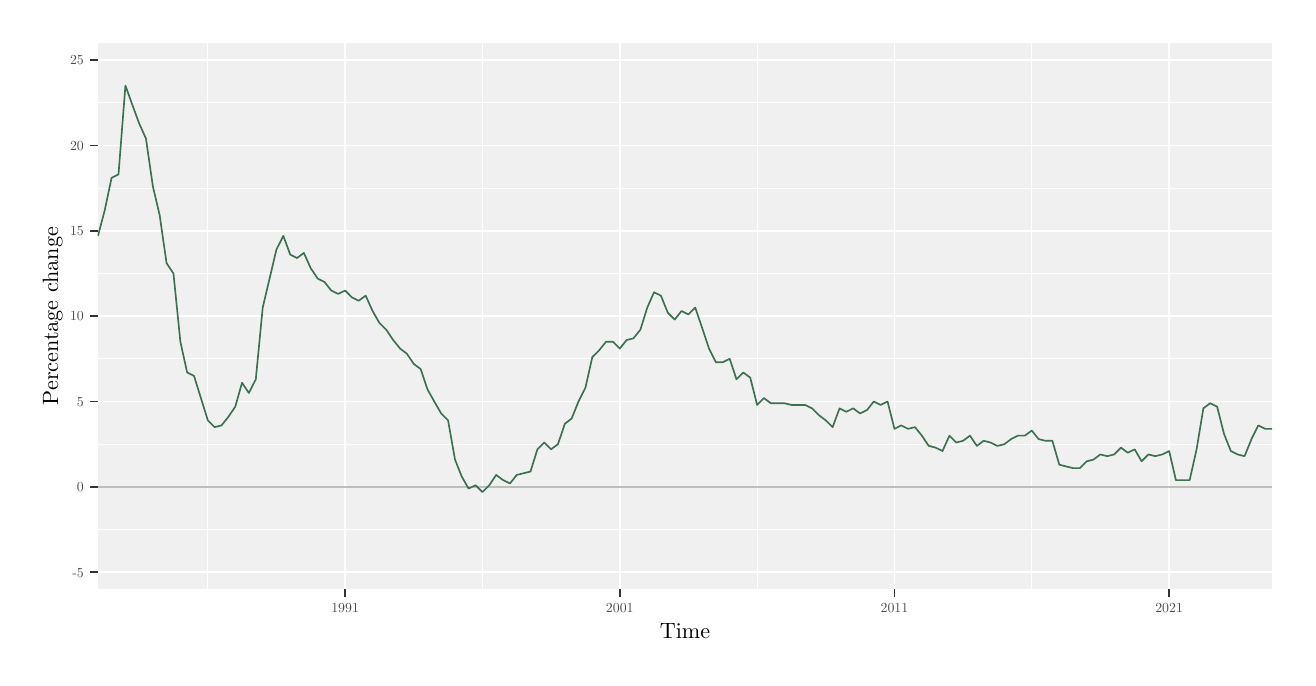
\begin{tikzpicture}[x=1pt,y=1pt]
\definecolor{fillColor}{RGB}{255,255,255}
\path[use as bounding box,fill=fillColor,fill opacity=0.00] (0,0) rectangle (455.30,227.65);
\begin{scope}
\path[clip] (  0.00,  0.00) rectangle (455.30,227.65);
\definecolor{drawColor}{RGB}{255,255,255}
\definecolor{fillColor}{RGB}{255,255,255}

\path[draw=drawColor,line width= 0.6pt,line join=round,line cap=round,fill=fillColor] (  0.00,  0.00) rectangle (455.30,227.65);
\end{scope}
\begin{scope}
\path[clip] ( 25.26, 24.68) rectangle (449.80,222.15);
\definecolor{fillColor}{gray}{0.94}

\path[fill=fillColor] ( 25.26, 24.68) rectangle (449.80,222.15);
\definecolor{drawColor}{RGB}{255,255,255}

\path[draw=drawColor,line width= 0.3pt,line join=round] ( 25.26, 46.28) --
	(449.80, 46.28);

\path[draw=drawColor,line width= 0.3pt,line join=round] ( 25.26, 77.13) --
	(449.80, 77.13);

\path[draw=drawColor,line width= 0.3pt,line join=round] ( 25.26,107.99) --
	(449.80,107.99);

\path[draw=drawColor,line width= 0.3pt,line join=round] ( 25.26,138.84) --
	(449.80,138.84);

\path[draw=drawColor,line width= 0.3pt,line join=round] ( 25.26,169.70) --
	(449.80,169.70);

\path[draw=drawColor,line width= 0.3pt,line join=round] ( 25.26,200.55) --
	(449.80,200.55);

\path[draw=drawColor,line width= 0.3pt,line join=round] ( 65.10, 24.68) --
	( 65.10,222.15);

\path[draw=drawColor,line width= 0.3pt,line join=round] (164.34, 24.68) --
	(164.34,222.15);

\path[draw=drawColor,line width= 0.3pt,line join=round] (263.59, 24.68) --
	(263.59,222.15);

\path[draw=drawColor,line width= 0.3pt,line join=round] (362.84, 24.68) --
	(362.84,222.15);

\path[draw=drawColor,line width= 0.6pt,line join=round] ( 25.26, 30.85) --
	(449.80, 30.85);

\path[draw=drawColor,line width= 0.6pt,line join=round] ( 25.26, 61.71) --
	(449.80, 61.71);

\path[draw=drawColor,line width= 0.6pt,line join=round] ( 25.26, 92.56) --
	(449.80, 92.56);

\path[draw=drawColor,line width= 0.6pt,line join=round] ( 25.26,123.42) --
	(449.80,123.42);

\path[draw=drawColor,line width= 0.6pt,line join=round] ( 25.26,154.27) --
	(449.80,154.27);

\path[draw=drawColor,line width= 0.6pt,line join=round] ( 25.26,185.12) --
	(449.80,185.12);

\path[draw=drawColor,line width= 0.6pt,line join=round] ( 25.26,215.98) --
	(449.80,215.98);

\path[draw=drawColor,line width= 0.6pt,line join=round] (114.71, 24.68) --
	(114.71,222.15);

\path[draw=drawColor,line width= 0.6pt,line join=round] (213.97, 24.68) --
	(213.97,222.15);

\path[draw=drawColor,line width= 0.6pt,line join=round] (313.21, 24.68) --
	(313.21,222.15);

\path[draw=drawColor,line width= 0.6pt,line join=round] (412.47, 24.68) --
	(412.47,222.15);
\definecolor{drawColor}{RGB}{190,190,190}

\path[draw=drawColor,line width= 0.6pt,line join=round] ( 25.26, 61.71) -- (449.80, 61.71);
\definecolor{drawColor}{RGB}{60,113,79}

\path[draw=drawColor,line width= 0.6pt,line join=round] ( 25.40,152.42) --
	( 27.85,161.68) --
	( 30.32,173.40) --
	( 32.82,174.63) --
	( 35.32,206.72) --
	( 37.76,199.94) --
	( 40.24,193.15) --
	( 42.74,187.59) --
	( 45.24,170.31) --
	( 47.71,159.82) --
	( 50.18,142.55) --
	( 52.68,138.84) --
	( 55.18,114.16) --
	( 57.63,103.05) --
	( 60.10,101.82) --
	( 62.60, 93.80) --
	( 65.10, 85.77) --
	( 67.54, 83.30) --
	( 70.02, 83.92) --
	( 72.52, 87.01) --
	( 75.02, 90.71) --
	( 77.46, 99.35) --
	( 79.93, 95.65) --
	( 82.43,100.58) --
	( 84.93,126.50) --
	( 87.41,136.99) --
	( 89.88,147.48) --
	( 92.38,152.42) --
	( 94.88,145.63) --
	( 97.32,144.40) --
	( 99.80,146.25) --
	(102.30,140.69) --
	(104.80,136.99) --
	(107.24,135.76) --
	(109.71,132.67) --
	(112.21,131.44) --
	(114.71,132.67) --
	(117.16,130.20) --
	(119.63,128.97) --
	(122.13,130.82) --
	(124.63,125.27) --
	(127.10,120.95) --
	(129.58,118.48) --
	(132.08,114.78) --
	(134.58,111.69) --
	(137.02,109.84) --
	(139.50,106.14) --
	(142.00,104.29) --
	(144.50, 96.88) --
	(146.94, 92.56) --
	(149.41, 88.24) --
	(151.91, 85.77) --
	(154.41, 71.58) --
	(156.86, 65.41) --
	(159.33, 61.09) --
	(161.83, 62.32) --
	(164.33, 59.85) --
	(166.80, 62.32) --
	(169.28, 66.03) --
	(171.78, 64.17) --
	(174.28, 62.94) --
	(176.72, 66.03) --
	(179.19, 66.64) --
	(181.69, 67.26) --
	(184.19, 75.28) --
	(186.64, 77.75) --
	(189.11, 75.28) --
	(191.61, 77.13) --
	(194.11, 84.54) --
	(196.56, 86.39) --
	(199.03, 92.56) --
	(201.53, 97.50) --
	(204.03,108.61) --
	(206.50,111.07) --
	(208.97,114.16) --
	(211.47,114.16) --
	(213.97,111.69) --
	(216.42,114.78) --
	(218.89,115.39) --
	(221.39,118.48) --
	(223.89,126.50) --
	(226.34,132.05) --
	(228.81,130.82) --
	(231.31,124.65) --
	(233.81,122.18) --
	(236.26,125.27) --
	(238.73,124.03) --
	(241.23,126.50) --
	(243.73,119.10) --
	(246.20,111.69) --
	(248.67,106.75) --
	(251.17,106.75) --
	(253.67,107.99) --
	(256.12,100.58) --
	(258.59,103.05) --
	(261.09,101.20) --
	(263.59, 91.33) --
	(266.04, 93.80) --
	(268.51, 91.94) --
	(271.01, 91.94) --
	(273.51, 91.94) --
	(275.95, 91.33) --
	(278.43, 91.33) --
	(280.93, 91.33) --
	(283.43, 90.09) --
	(285.90, 87.62) --
	(288.37, 85.77) --
	(290.87, 83.30) --
	(293.37, 90.09) --
	(295.82, 88.86) --
	(298.29, 90.09) --
	(300.79, 88.24) --
	(303.29, 89.48) --
	(305.73, 92.56) --
	(308.21, 91.33) --
	(310.71, 92.56) --
	(313.21, 82.69) --
	(315.65, 83.92) --
	(318.12, 82.69) --
	(320.62, 83.30) --
	(323.12, 80.22) --
	(325.60, 76.52) --
	(328.07, 75.90) --
	(330.57, 74.67) --
	(333.07, 80.22) --
	(335.52, 77.75) --
	(337.99, 78.37) --
	(340.49, 80.22) --
	(342.99, 76.52) --
	(345.43, 78.37) --
	(347.91, 77.75) --
	(350.41, 76.52) --
	(352.91, 77.13) --
	(355.35, 78.98) --
	(357.82, 80.22) --
	(360.32, 80.22) --
	(362.82, 82.07) --
	(365.30, 78.98) --
	(367.77, 78.37) --
	(370.27, 78.37) --
	(372.77, 69.73) --
	(375.21, 69.11) --
	(377.69, 68.49) --
	(380.19, 68.49) --
	(382.69, 70.96) --
	(385.13, 71.58) --
	(387.60, 73.43) --
	(390.10, 72.81) --
	(392.60, 73.43) --
	(395.05, 75.90) --
	(397.52, 74.05) --
	(400.02, 75.28) --
	(402.52, 70.96) --
	(404.99, 73.43) --
	(407.47, 72.81) --
	(409.97, 73.43) --
	(412.47, 74.67) --
	(414.91, 64.17) --
	(417.38, 64.17) --
	(419.88, 64.17) --
	(422.38, 75.28) --
	(424.83, 90.09) --
	(427.30, 91.94) --
	(429.80, 90.71) --
	(432.30, 80.84) --
	(434.75, 74.67) --
	(437.22, 73.43) --
	(439.72, 72.81) --
	(442.22, 78.98) --
	(444.69, 83.92) --
	(447.17, 82.69) --
	(449.67, 82.69);
\end{scope}
\begin{scope}
\path[clip] (  0.00,  0.00) rectangle (455.30,227.65);
\definecolor{drawColor}{gray}{0.30}

\node[text=drawColor,anchor=base east,inner sep=0pt, outer sep=0pt, scale=  0.50] at ( 20.31, 29.13) {-5};

\node[text=drawColor,anchor=base east,inner sep=0pt, outer sep=0pt, scale=  0.50] at ( 20.31, 59.98) {0};

\node[text=drawColor,anchor=base east,inner sep=0pt, outer sep=0pt, scale=  0.50] at ( 20.31, 90.84) {5};

\node[text=drawColor,anchor=base east,inner sep=0pt, outer sep=0pt, scale=  0.50] at ( 20.31,121.69) {10};

\node[text=drawColor,anchor=base east,inner sep=0pt, outer sep=0pt, scale=  0.50] at ( 20.31,152.55) {15};

\node[text=drawColor,anchor=base east,inner sep=0pt, outer sep=0pt, scale=  0.50] at ( 20.31,183.40) {20};

\node[text=drawColor,anchor=base east,inner sep=0pt, outer sep=0pt, scale=  0.50] at ( 20.31,214.26) {25};
\end{scope}
\begin{scope}
\path[clip] (  0.00,  0.00) rectangle (455.30,227.65);
\definecolor{drawColor}{gray}{0.20}

\path[draw=drawColor,line width= 0.6pt,line join=round] ( 22.51, 30.85) --
	( 25.26, 30.85);

\path[draw=drawColor,line width= 0.6pt,line join=round] ( 22.51, 61.71) --
	( 25.26, 61.71);

\path[draw=drawColor,line width= 0.6pt,line join=round] ( 22.51, 92.56) --
	( 25.26, 92.56);

\path[draw=drawColor,line width= 0.6pt,line join=round] ( 22.51,123.42) --
	( 25.26,123.42);

\path[draw=drawColor,line width= 0.6pt,line join=round] ( 22.51,154.27) --
	( 25.26,154.27);

\path[draw=drawColor,line width= 0.6pt,line join=round] ( 22.51,185.12) --
	( 25.26,185.12);

\path[draw=drawColor,line width= 0.6pt,line join=round] ( 22.51,215.98) --
	( 25.26,215.98);
\end{scope}
\begin{scope}
\path[clip] (  0.00,  0.00) rectangle (455.30,227.65);
\definecolor{drawColor}{gray}{0.20}

\path[draw=drawColor,line width= 0.6pt,line join=round] (114.71, 21.93) --
	(114.71, 24.68);

\path[draw=drawColor,line width= 0.6pt,line join=round] (213.97, 21.93) --
	(213.97, 24.68);

\path[draw=drawColor,line width= 0.6pt,line join=round] (313.21, 21.93) --
	(313.21, 24.68);

\path[draw=drawColor,line width= 0.6pt,line join=round] (412.47, 21.93) --
	(412.47, 24.68);
\end{scope}
\begin{scope}
\path[clip] (  0.00,  0.00) rectangle (455.30,227.65);
\definecolor{drawColor}{gray}{0.30}

\node[text=drawColor,anchor=base,inner sep=0pt, outer sep=0pt, scale=  0.50] at (114.71, 16.29) {1991};

\node[text=drawColor,anchor=base,inner sep=0pt, outer sep=0pt, scale=  0.50] at (213.97, 16.29) {2001};

\node[text=drawColor,anchor=base,inner sep=0pt, outer sep=0pt, scale=  0.50] at (313.21, 16.29) {2011};

\node[text=drawColor,anchor=base,inner sep=0pt, outer sep=0pt, scale=  0.50] at (412.47, 16.29) {2021};
\end{scope}
\begin{scope}
\path[clip] (  0.00,  0.00) rectangle (455.30,227.65);
\definecolor{drawColor}{RGB}{0,0,0}

\node[text=drawColor,anchor=base,inner sep=0pt, outer sep=0pt, scale=  0.80] at (237.53,  7.06) {Time};
\end{scope}
\begin{scope}
\path[clip] (  0.00,  0.00) rectangle (455.30,227.65);
\definecolor{drawColor}{RGB}{0,0,0}

\node[text=drawColor,rotate= 90.00,anchor=base,inner sep=0pt, outer sep=0pt, scale=  0.80] at ( 11.01,123.42) {Percentage change};
\end{scope}
\end{tikzpicture}

  \label{fig:eci}
\end{figure}

As relates to the (1), the identify 4 types of affected actors: employers, governments, the medical sector as a business sector (doctors, hospitals) and workers. To investigate the employer costs, the authors cite \textcite[][]{Claxton2011} who assemble National Compensation Survey data for mean health insurance costs per worker hour. \textcite[][]{Claxton2011} present data that shows that employers' cost had doubled in 2010 (\$1.60) compared to 1999 (\$3.35). However, there appear to be some issues with the data: First, \textcite[][]{Jacobs2014} cite this change as \enquote{more than 50\%} \pnotecite[p. 451]{Jacobs2014}, which is technically correct, but odd considering the increase is greater than 100\%. Second, I was not able to reproduce the exact data values reported by \textcite[][]{Claxton2011} using, to the best of my knowledge, the same data source (Employer Cost for Employee Compensation data derived from the National Compensation Survey (ECEC); \nptextcite{ECEC}), as they do not clearly state how they compiled their data. Nevertheless, using the ECEC data I was able to retrieve, the finding for the relative increase still holds, more than doubling from \$1.18 in 1999 to \$2.48 in 2010 (see \hyperref[fig:ecec]{Figure 2}).

\begin{figure}[H]
  \sffamily
  \caption{Employer Costs for Employee Compensation 1993--2024}
  % Created by tikzDevice version 0.12.6 on 2025-02-16 03:22:09
% !TEX encoding = UTF-8 Unicode
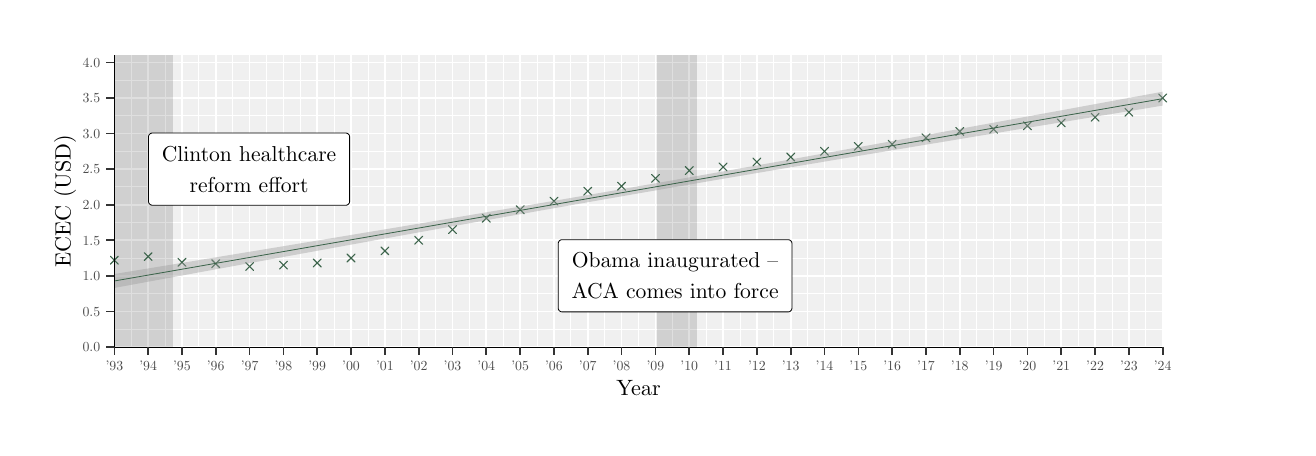
\begin{tikzpicture}[x=1pt,y=1pt]
\definecolor{fillColor}{RGB}{255,255,255}
\path[use as bounding box,fill=fillColor,fill opacity=0.00] (0,0) rectangle (455.30,144.54);
\begin{scope}
\path[clip] (  0.00,  0.00) rectangle (455.30,144.54);
\definecolor{drawColor}{RGB}{255,255,255}
\definecolor{fillColor}{RGB}{255,255,255}

\path[draw=drawColor,line width= 0.6pt,line join=round,line cap=round,fill=fillColor] ( -0.00,  0.00) rectangle (455.30,144.54);
\end{scope}
\begin{scope}
\path[clip] (  0.00,  0.00) rectangle (455.30,144.54);
\definecolor{fillColor}{gray}{0.94}

\path[fill=fillColor] ( 31.15, 29.18) rectangle (410.30,134.54);
\definecolor{drawColor}{RGB}{255,255,255}

\path[draw=drawColor,line width= 0.3pt,line join=round] ( 31.15, 35.60) --
	(410.30, 35.60);

\path[draw=drawColor,line width= 0.3pt,line join=round] ( 31.15, 48.45) --
	(410.30, 48.45);

\path[draw=drawColor,line width= 0.3pt,line join=round] ( 31.15, 61.30) --
	(410.30, 61.30);

\path[draw=drawColor,line width= 0.3pt,line join=round] ( 31.15, 74.15) --
	(410.30, 74.15);

\path[draw=drawColor,line width= 0.3pt,line join=round] ( 31.15, 87.00) --
	(410.30, 87.00);

\path[draw=drawColor,line width= 0.3pt,line join=round] ( 31.15, 99.85) --
	(410.30, 99.85);

\path[draw=drawColor,line width= 0.3pt,line join=round] ( 31.15,112.70) --
	(410.30,112.70);

\path[draw=drawColor,line width= 0.3pt,line join=round] ( 31.15,125.55) --
	(410.30,125.55);

\path[draw=drawColor,line width= 0.3pt,line join=round] ( 37.43, 29.18) --
	( 37.43,134.54);

\path[draw=drawColor,line width= 0.3pt,line join=round] ( 49.64, 29.18) --
	( 49.64,134.54);

\path[draw=drawColor,line width= 0.3pt,line join=round] ( 61.85, 29.18) --
	( 61.85,134.54);

\path[draw=drawColor,line width= 0.3pt,line join=round] ( 74.08, 29.18) --
	( 74.08,134.54);

\path[draw=drawColor,line width= 0.3pt,line join=round] ( 86.31, 29.18) --
	( 86.31,134.54);

\path[draw=drawColor,line width= 0.3pt,line join=round] ( 98.52, 29.18) --
	( 98.52,134.54);

\path[draw=drawColor,line width= 0.3pt,line join=round] (110.73, 29.18) --
	(110.73,134.54);

\path[draw=drawColor,line width= 0.3pt,line join=round] (122.96, 29.18) --
	(122.96,134.54);

\path[draw=drawColor,line width= 0.3pt,line join=round] (135.19, 29.18) --
	(135.19,134.54);

\path[draw=drawColor,line width= 0.3pt,line join=round] (147.40, 29.18) --
	(147.40,134.54);

\path[draw=drawColor,line width= 0.3pt,line join=round] (159.62, 29.18) --
	(159.62,134.54);

\path[draw=drawColor,line width= 0.3pt,line join=round] (171.84, 29.18) --
	(171.84,134.54);

\path[draw=drawColor,line width= 0.3pt,line join=round] (184.07, 29.18) --
	(184.07,134.54);

\path[draw=drawColor,line width= 0.3pt,line join=round] (196.29, 29.18) --
	(196.29,134.54);

\path[draw=drawColor,line width= 0.3pt,line join=round] (208.50, 29.18) --
	(208.50,134.54);

\path[draw=drawColor,line width= 0.3pt,line join=round] (220.73, 29.18) --
	(220.73,134.54);

\path[draw=drawColor,line width= 0.3pt,line join=round] (232.96, 29.18) --
	(232.96,134.54);

\path[draw=drawColor,line width= 0.3pt,line join=round] (245.17, 29.18) --
	(245.17,134.54);

\path[draw=drawColor,line width= 0.3pt,line join=round] (257.38, 29.18) --
	(257.38,134.54);

\path[draw=drawColor,line width= 0.3pt,line join=round] (269.61, 29.18) --
	(269.61,134.54);

\path[draw=drawColor,line width= 0.3pt,line join=round] (281.84, 29.18) --
	(281.84,134.54);

\path[draw=drawColor,line width= 0.3pt,line join=round] (294.05, 29.18) --
	(294.05,134.54);

\path[draw=drawColor,line width= 0.3pt,line join=round] (306.26, 29.18) --
	(306.26,134.54);

\path[draw=drawColor,line width= 0.3pt,line join=round] (318.49, 29.18) --
	(318.49,134.54);

\path[draw=drawColor,line width= 0.3pt,line join=round] (330.72, 29.18) --
	(330.72,134.54);

\path[draw=drawColor,line width= 0.3pt,line join=round] (342.93, 29.18) --
	(342.93,134.54);

\path[draw=drawColor,line width= 0.3pt,line join=round] (355.15, 29.18) --
	(355.15,134.54);

\path[draw=drawColor,line width= 0.3pt,line join=round] (367.37, 29.18) --
	(367.37,134.54);

\path[draw=drawColor,line width= 0.3pt,line join=round] (379.60, 29.18) --
	(379.60,134.54);

\path[draw=drawColor,line width= 0.3pt,line join=round] (391.82, 29.18) --
	(391.82,134.54);

\path[draw=drawColor,line width= 0.3pt,line join=round] (404.03, 29.18) --
	(404.03,134.54);

\path[draw=drawColor,line width= 0.6pt,line join=round] ( 31.15, 29.18) --
	(410.30, 29.18);

\path[draw=drawColor,line width= 0.6pt,line join=round] ( 31.15, 42.03) --
	(410.30, 42.03);

\path[draw=drawColor,line width= 0.6pt,line join=round] ( 31.15, 54.88) --
	(410.30, 54.88);

\path[draw=drawColor,line width= 0.6pt,line join=round] ( 31.15, 67.73) --
	(410.30, 67.73);

\path[draw=drawColor,line width= 0.6pt,line join=round] ( 31.15, 80.58) --
	(410.30, 80.58);

\path[draw=drawColor,line width= 0.6pt,line join=round] ( 31.15, 93.42) --
	(410.30, 93.42);

\path[draw=drawColor,line width= 0.6pt,line join=round] ( 31.15,106.27) --
	(410.30,106.27);

\path[draw=drawColor,line width= 0.6pt,line join=round] ( 31.15,119.12) --
	(410.30,119.12);

\path[draw=drawColor,line width= 0.6pt,line join=round] ( 31.15,131.97) --
	(410.30,131.97);

\path[draw=drawColor,line width= 0.6pt,line join=round] ( 31.32, 29.18) --
	( 31.32,134.54);

\path[draw=drawColor,line width= 0.6pt,line join=round] ( 43.53, 29.18) --
	( 43.53,134.54);

\path[draw=drawColor,line width= 0.6pt,line join=round] ( 55.74, 29.18) --
	( 55.74,134.54);

\path[draw=drawColor,line width= 0.6pt,line join=round] ( 67.96, 29.18) --
	( 67.96,134.54);

\path[draw=drawColor,line width= 0.6pt,line join=round] ( 80.20, 29.18) --
	( 80.20,134.54);

\path[draw=drawColor,line width= 0.6pt,line join=round] ( 92.41, 29.18) --
	( 92.41,134.54);

\path[draw=drawColor,line width= 0.6pt,line join=round] (104.63, 29.18) --
	(104.63,134.54);

\path[draw=drawColor,line width= 0.6pt,line join=round] (116.84, 29.18) --
	(116.84,134.54);

\path[draw=drawColor,line width= 0.6pt,line join=round] (129.08, 29.18) --
	(129.08,134.54);

\path[draw=drawColor,line width= 0.6pt,line join=round] (141.30, 29.18) --
	(141.30,134.54);

\path[draw=drawColor,line width= 0.6pt,line join=round] (153.51, 29.18) --
	(153.51,134.54);

\path[draw=drawColor,line width= 0.6pt,line join=round] (165.72, 29.18) --
	(165.72,134.54);

\path[draw=drawColor,line width= 0.6pt,line join=round] (177.97, 29.18) --
	(177.97,134.54);

\path[draw=drawColor,line width= 0.6pt,line join=round] (190.18, 29.18) --
	(190.18,134.54);

\path[draw=drawColor,line width= 0.6pt,line join=round] (202.39, 29.18) --
	(202.39,134.54);

\path[draw=drawColor,line width= 0.6pt,line join=round] (214.60, 29.18) --
	(214.60,134.54);

\path[draw=drawColor,line width= 0.6pt,line join=round] (226.85, 29.18) --
	(226.85,134.54);

\path[draw=drawColor,line width= 0.6pt,line join=round] (239.06, 29.18) --
	(239.06,134.54);

\path[draw=drawColor,line width= 0.6pt,line join=round] (251.27, 29.18) --
	(251.27,134.54);

\path[draw=drawColor,line width= 0.6pt,line join=round] (263.49, 29.18) --
	(263.49,134.54);

\path[draw=drawColor,line width= 0.6pt,line join=round] (275.73, 29.18) --
	(275.73,134.54);

\path[draw=drawColor,line width= 0.6pt,line join=round] (287.94, 29.18) --
	(287.94,134.54);

\path[draw=drawColor,line width= 0.6pt,line join=round] (300.16, 29.18) --
	(300.16,134.54);

\path[draw=drawColor,line width= 0.6pt,line join=round] (312.37, 29.18) --
	(312.37,134.54);

\path[draw=drawColor,line width= 0.6pt,line join=round] (324.61, 29.18) --
	(324.61,134.54);

\path[draw=drawColor,line width= 0.6pt,line join=round] (336.83, 29.18) --
	(336.83,134.54);

\path[draw=drawColor,line width= 0.6pt,line join=round] (349.04, 29.18) --
	(349.04,134.54);

\path[draw=drawColor,line width= 0.6pt,line join=round] (361.25, 29.18) --
	(361.25,134.54);

\path[draw=drawColor,line width= 0.6pt,line join=round] (373.50, 29.18) --
	(373.50,134.54);

\path[draw=drawColor,line width= 0.6pt,line join=round] (385.71, 29.18) --
	(385.71,134.54);

\path[draw=drawColor,line width= 0.6pt,line join=round] (397.92, 29.18) --
	(397.92,134.54);

\path[draw=drawColor,line width= 0.6pt,line join=round] (410.13, 29.18) --
	(410.13,134.54);
\definecolor{fillColor}{RGB}{190,190,190}

\path[fill=fillColor,fill opacity=0.01] ( 31.32, 29.18) rectangle ( 52.50,134.54);

\path[fill=fillColor,fill opacity=0.01] ( 31.32, 29.18) rectangle ( 52.50,134.54);

\path[fill=fillColor,fill opacity=0.01] ( 31.32, 29.18) rectangle ( 52.50,134.54);

\path[fill=fillColor,fill opacity=0.01] ( 31.32, 29.18) rectangle ( 52.50,134.54);

\path[fill=fillColor,fill opacity=0.01] ( 31.32, 29.18) rectangle ( 52.50,134.54);

\path[fill=fillColor,fill opacity=0.01] ( 31.32, 29.18) rectangle ( 52.50,134.54);

\path[fill=fillColor,fill opacity=0.01] ( 31.32, 29.18) rectangle ( 52.50,134.54);

\path[fill=fillColor,fill opacity=0.01] ( 31.32, 29.18) rectangle ( 52.50,134.54);

\path[fill=fillColor,fill opacity=0.01] ( 31.32, 29.18) rectangle ( 52.50,134.54);

\path[fill=fillColor,fill opacity=0.01] ( 31.32, 29.18) rectangle ( 52.50,134.54);

\path[fill=fillColor,fill opacity=0.01] ( 31.32, 29.18) rectangle ( 52.50,134.54);

\path[fill=fillColor,fill opacity=0.01] ( 31.32, 29.18) rectangle ( 52.50,134.54);

\path[fill=fillColor,fill opacity=0.01] ( 31.32, 29.18) rectangle ( 52.50,134.54);

\path[fill=fillColor,fill opacity=0.01] ( 31.32, 29.18) rectangle ( 52.50,134.54);

\path[fill=fillColor,fill opacity=0.01] ( 31.32, 29.18) rectangle ( 52.50,134.54);

\path[fill=fillColor,fill opacity=0.01] ( 31.32, 29.18) rectangle ( 52.50,134.54);

\path[fill=fillColor,fill opacity=0.01] ( 31.32, 29.18) rectangle ( 52.50,134.54);

\path[fill=fillColor,fill opacity=0.01] ( 31.32, 29.18) rectangle ( 52.50,134.54);

\path[fill=fillColor,fill opacity=0.01] ( 31.32, 29.18) rectangle ( 52.50,134.54);

\path[fill=fillColor,fill opacity=0.01] ( 31.32, 29.18) rectangle ( 52.50,134.54);

\path[fill=fillColor,fill opacity=0.01] ( 31.32, 29.18) rectangle ( 52.50,134.54);

\path[fill=fillColor,fill opacity=0.01] ( 31.32, 29.18) rectangle ( 52.50,134.54);

\path[fill=fillColor,fill opacity=0.01] ( 31.32, 29.18) rectangle ( 52.50,134.54);

\path[fill=fillColor,fill opacity=0.01] ( 31.32, 29.18) rectangle ( 52.50,134.54);

\path[fill=fillColor,fill opacity=0.01] ( 31.32, 29.18) rectangle ( 52.50,134.54);

\path[fill=fillColor,fill opacity=0.01] ( 31.32, 29.18) rectangle ( 52.50,134.54);

\path[fill=fillColor,fill opacity=0.01] ( 31.32, 29.18) rectangle ( 52.50,134.54);

\path[fill=fillColor,fill opacity=0.01] ( 31.32, 29.18) rectangle ( 52.50,134.54);

\path[fill=fillColor,fill opacity=0.01] ( 31.32, 29.18) rectangle ( 52.50,134.54);

\path[fill=fillColor,fill opacity=0.01] ( 31.32, 29.18) rectangle ( 52.50,134.54);

\path[fill=fillColor,fill opacity=0.01] ( 31.32, 29.18) rectangle ( 52.50,134.54);

\path[fill=fillColor,fill opacity=0.01] ( 31.32, 29.18) rectangle ( 52.50,134.54);

\path[fill=fillColor,fill opacity=0.01] (227.49, 29.18) rectangle (241.77,134.54);

\path[fill=fillColor,fill opacity=0.01] (227.49, 29.18) rectangle (241.77,134.54);

\path[fill=fillColor,fill opacity=0.01] (227.49, 29.18) rectangle (241.77,134.54);

\path[fill=fillColor,fill opacity=0.01] (227.49, 29.18) rectangle (241.77,134.54);

\path[fill=fillColor,fill opacity=0.01] (227.49, 29.18) rectangle (241.77,134.54);

\path[fill=fillColor,fill opacity=0.01] (227.49, 29.18) rectangle (241.77,134.54);

\path[fill=fillColor,fill opacity=0.01] (227.49, 29.18) rectangle (241.77,134.54);

\path[fill=fillColor,fill opacity=0.01] (227.49, 29.18) rectangle (241.77,134.54);

\path[fill=fillColor,fill opacity=0.01] (227.49, 29.18) rectangle (241.77,134.54);

\path[fill=fillColor,fill opacity=0.01] (227.49, 29.18) rectangle (241.77,134.54);

\path[fill=fillColor,fill opacity=0.01] (227.49, 29.18) rectangle (241.77,134.54);

\path[fill=fillColor,fill opacity=0.01] (227.49, 29.18) rectangle (241.77,134.54);

\path[fill=fillColor,fill opacity=0.01] (227.49, 29.18) rectangle (241.77,134.54);

\path[fill=fillColor,fill opacity=0.01] (227.49, 29.18) rectangle (241.77,134.54);

\path[fill=fillColor,fill opacity=0.01] (227.49, 29.18) rectangle (241.77,134.54);

\path[fill=fillColor,fill opacity=0.01] (227.49, 29.18) rectangle (241.77,134.54);

\path[fill=fillColor,fill opacity=0.01] (227.49, 29.18) rectangle (241.77,134.54);

\path[fill=fillColor,fill opacity=0.01] (227.49, 29.18) rectangle (241.77,134.54);

\path[fill=fillColor,fill opacity=0.01] (227.49, 29.18) rectangle (241.77,134.54);

\path[fill=fillColor,fill opacity=0.01] (227.49, 29.18) rectangle (241.77,134.54);

\path[fill=fillColor,fill opacity=0.01] (227.49, 29.18) rectangle (241.77,134.54);

\path[fill=fillColor,fill opacity=0.01] (227.49, 29.18) rectangle (241.77,134.54);

\path[fill=fillColor,fill opacity=0.01] (227.49, 29.18) rectangle (241.77,134.54);

\path[fill=fillColor,fill opacity=0.01] (227.49, 29.18) rectangle (241.77,134.54);

\path[fill=fillColor,fill opacity=0.01] (227.49, 29.18) rectangle (241.77,134.54);

\path[fill=fillColor,fill opacity=0.01] (227.49, 29.18) rectangle (241.77,134.54);

\path[fill=fillColor,fill opacity=0.01] (227.49, 29.18) rectangle (241.77,134.54);

\path[fill=fillColor,fill opacity=0.01] (227.49, 29.18) rectangle (241.77,134.54);

\path[fill=fillColor,fill opacity=0.01] (227.49, 29.18) rectangle (241.77,134.54);

\path[fill=fillColor,fill opacity=0.01] (227.49, 29.18) rectangle (241.77,134.54);

\path[fill=fillColor,fill opacity=0.01] (227.49, 29.18) rectangle (241.77,134.54);

\path[fill=fillColor,fill opacity=0.01] (227.49, 29.18) rectangle (241.77,134.54);
\definecolor{drawColor}{RGB}{60,100,75}

\path[draw=drawColor,line width= 0.4pt,line join=round,line cap=round] ( 29.89, 59.10) -- ( 32.75, 61.96);

\path[draw=drawColor,line width= 0.4pt,line join=round,line cap=round] ( 29.89, 61.96) -- ( 32.75, 59.10);

\path[draw=drawColor,line width= 0.4pt,line join=round,line cap=round] ( 42.11, 60.39) -- ( 44.96, 63.24);

\path[draw=drawColor,line width= 0.4pt,line join=round,line cap=round] ( 42.11, 63.24) -- ( 44.96, 60.39);

\path[draw=drawColor,line width= 0.4pt,line join=round,line cap=round] ( 54.32, 58.33) -- ( 57.17, 61.19);

\path[draw=drawColor,line width= 0.4pt,line join=round,line cap=round] ( 54.32, 61.19) -- ( 57.17, 58.33);

\path[draw=drawColor,line width= 0.4pt,line join=round,line cap=round] ( 66.53, 57.82) -- ( 69.38, 60.67);

\path[draw=drawColor,line width= 0.4pt,line join=round,line cap=round] ( 66.53, 60.67) -- ( 69.38, 57.82);

\path[draw=drawColor,line width= 0.4pt,line join=round,line cap=round] ( 78.78, 56.79) -- ( 81.63, 59.65);

\path[draw=drawColor,line width= 0.4pt,line join=round,line cap=round] ( 78.78, 59.65) -- ( 81.63, 56.79);

\path[draw=drawColor,line width= 0.4pt,line join=round,line cap=round] ( 90.99, 57.31) -- ( 93.84, 60.16);

\path[draw=drawColor,line width= 0.4pt,line join=round,line cap=round] ( 90.99, 60.16) -- ( 93.84, 57.31);

\path[draw=drawColor,line width= 0.4pt,line join=round,line cap=round] (103.20, 58.08) -- (106.05, 60.93);

\path[draw=drawColor,line width= 0.4pt,line join=round,line cap=round] (103.20, 60.93) -- (106.05, 58.08);

\path[draw=drawColor,line width= 0.4pt,line join=round,line cap=round] (115.41, 59.88) -- (118.27, 62.73);

\path[draw=drawColor,line width= 0.4pt,line join=round,line cap=round] (115.41, 62.73) -- (118.27, 59.88);

\path[draw=drawColor,line width= 0.4pt,line join=round,line cap=round] (127.66, 62.45) -- (130.51, 65.30);

\path[draw=drawColor,line width= 0.4pt,line join=round,line cap=round] (127.66, 65.30) -- (130.51, 62.45);

\path[draw=drawColor,line width= 0.4pt,line join=round,line cap=round] (139.87, 66.30) -- (142.72, 69.15);

\path[draw=drawColor,line width= 0.4pt,line join=round,line cap=round] (139.87, 69.15) -- (142.72, 66.30);

\path[draw=drawColor,line width= 0.4pt,line join=round,line cap=round] (152.08, 70.15) -- (154.94, 73.01);

\path[draw=drawColor,line width= 0.4pt,line join=round,line cap=round] (152.08, 73.01) -- (154.94, 70.15);

\path[draw=drawColor,line width= 0.4pt,line join=round,line cap=round] (164.29, 74.27) -- (167.15, 77.12);

\path[draw=drawColor,line width= 0.4pt,line join=round,line cap=round] (164.29, 77.12) -- (167.15, 74.27);

\path[draw=drawColor,line width= 0.4pt,line join=round,line cap=round] (176.54, 77.35) -- (179.39, 80.20);

\path[draw=drawColor,line width= 0.4pt,line join=round,line cap=round] (176.54, 80.20) -- (179.39, 77.35);

\path[draw=drawColor,line width= 0.4pt,line join=round,line cap=round] (188.75, 80.43) -- (191.61, 83.29);

\path[draw=drawColor,line width= 0.4pt,line join=round,line cap=round] (188.75, 83.29) -- (191.61, 80.43);

\path[draw=drawColor,line width= 0.4pt,line join=round,line cap=round] (200.96, 84.03) -- (203.82, 86.88);

\path[draw=drawColor,line width= 0.4pt,line join=round,line cap=round] (200.96, 86.88) -- (203.82, 84.03);

\path[draw=drawColor,line width= 0.4pt,line join=round,line cap=round] (213.18, 85.83) -- (216.03, 88.68);

\path[draw=drawColor,line width= 0.4pt,line join=round,line cap=round] (213.18, 88.68) -- (216.03, 85.83);

\path[draw=drawColor,line width= 0.4pt,line join=round,line cap=round] (225.42, 88.66) -- (228.28, 91.51);

\path[draw=drawColor,line width= 0.4pt,line join=round,line cap=round] (225.42, 91.51) -- (228.28, 88.66);

\path[draw=drawColor,line width= 0.4pt,line join=round,line cap=round] (237.64, 91.48) -- (240.49, 94.34);

\path[draw=drawColor,line width= 0.4pt,line join=round,line cap=round] (237.64, 94.34) -- (240.49, 91.48);

\path[draw=drawColor,line width= 0.4pt,line join=round,line cap=round] (249.85, 92.77) -- (252.70, 95.62);

\path[draw=drawColor,line width= 0.4pt,line join=round,line cap=round] (249.85, 95.62) -- (252.70, 92.77);

\path[draw=drawColor,line width= 0.4pt,line join=round,line cap=round] (262.06, 94.57) -- (264.91, 97.42);

\path[draw=drawColor,line width= 0.4pt,line join=round,line cap=round] (262.06, 97.42) -- (264.91, 94.57);

\path[draw=drawColor,line width= 0.4pt,line join=round,line cap=round] (274.31, 96.37) -- (277.16, 99.22);

\path[draw=drawColor,line width= 0.4pt,line join=round,line cap=round] (274.31, 99.22) -- (277.16, 96.37);

\path[draw=drawColor,line width= 0.4pt,line join=round,line cap=round] (286.52, 98.42) -- (289.37,101.28);

\path[draw=drawColor,line width= 0.4pt,line join=round,line cap=round] (286.52,101.28) -- (289.37, 98.42);

\path[draw=drawColor,line width= 0.4pt,line join=round,line cap=round] (298.73,100.22) -- (301.58,103.07);

\path[draw=drawColor,line width= 0.4pt,line join=round,line cap=round] (298.73,103.07) -- (301.58,100.22);

\path[draw=drawColor,line width= 0.4pt,line join=round,line cap=round] (310.94,100.99) -- (313.80,103.84);

\path[draw=drawColor,line width= 0.4pt,line join=round,line cap=round] (310.94,103.84) -- (313.80,100.99);

\path[draw=drawColor,line width= 0.4pt,line join=round,line cap=round] (323.19,103.30) -- (326.04,106.16);

\path[draw=drawColor,line width= 0.4pt,line join=round,line cap=round] (323.19,106.16) -- (326.04,103.30);

\path[draw=drawColor,line width= 0.4pt,line join=round,line cap=round] (335.40,105.62) -- (338.25,108.47);

\path[draw=drawColor,line width= 0.4pt,line join=round,line cap=round] (335.40,108.47) -- (338.25,105.62);

\path[draw=drawColor,line width= 0.4pt,line join=round,line cap=round] (347.61,106.39) -- (350.47,109.24);

\path[draw=drawColor,line width= 0.4pt,line join=round,line cap=round] (347.61,109.24) -- (350.47,106.39);

\path[draw=drawColor,line width= 0.4pt,line join=round,line cap=round] (359.82,107.67) -- (362.68,110.53);

\path[draw=drawColor,line width= 0.4pt,line join=round,line cap=round] (359.82,110.53) -- (362.68,107.67);

\path[draw=drawColor,line width= 0.4pt,line join=round,line cap=round] (372.07,108.70) -- (374.92,111.55);

\path[draw=drawColor,line width= 0.4pt,line join=round,line cap=round] (372.07,111.55) -- (374.92,108.70);

\path[draw=drawColor,line width= 0.4pt,line join=round,line cap=round] (384.28,110.76) -- (387.14,113.61);

\path[draw=drawColor,line width= 0.4pt,line join=round,line cap=round] (384.28,113.61) -- (387.14,110.76);

\path[draw=drawColor,line width= 0.4pt,line join=round,line cap=round] (396.49,112.56) -- (399.35,115.41);

\path[draw=drawColor,line width= 0.4pt,line join=round,line cap=round] (396.49,115.41) -- (399.35,112.56);

\path[draw=drawColor,line width= 0.4pt,line join=round,line cap=round] (408.71,117.69) -- (411.56,120.55);

\path[draw=drawColor,line width= 0.4pt,line join=round,line cap=round] (408.71,120.55) -- (411.56,117.69);
\definecolor{fillColor}{RGB}{153,153,153}

\path[fill=fillColor,fill opacity=0.40] ( 31.32, 55.52) --
	( 36.11, 56.30) --
	( 40.91, 57.09) --
	( 45.70, 57.88) --
	( 50.50, 58.67) --
	( 55.30, 59.46) --
	( 60.09, 60.25) --
	( 64.89, 61.04) --
	( 69.68, 61.83) --
	( 74.48, 62.62) --
	( 79.27, 63.41) --
	( 84.07, 64.20) --
	( 88.86, 64.99) --
	( 93.66, 65.78) --
	( 98.45, 66.58) --
	(103.25, 67.37) --
	(108.04, 68.17) --
	(112.84, 68.96) --
	(117.63, 69.76) --
	(122.43, 70.56) --
	(127.22, 71.35) --
	(132.02, 72.15) --
	(136.81, 72.95) --
	(141.61, 73.76) --
	(146.40, 74.56) --
	(151.20, 75.36) --
	(155.99, 76.17) --
	(160.79, 76.98) --
	(165.58, 77.79) --
	(170.38, 78.60) --
	(175.17, 79.41) --
	(179.97, 80.23) --
	(184.76, 81.04) --
	(189.56, 81.86) --
	(194.35, 82.68) --
	(199.15, 83.50) --
	(203.94, 84.33) --
	(208.74, 85.15) --
	(213.53, 85.98) --
	(218.33, 86.82) --
	(223.12, 87.65) --
	(227.92, 88.49) --
	(232.71, 89.32) --
	(237.51, 90.17) --
	(242.30, 91.01) --
	(247.10, 91.85) --
	(251.89, 92.70) --
	(256.69, 93.55) --
	(261.49, 94.40) --
	(266.28, 95.26) --
	(271.08, 96.11) --
	(275.87, 96.97) --
	(280.67, 97.83) --
	(285.46, 98.69) --
	(290.26, 99.55) --
	(295.05,100.41) --
	(299.85,101.28) --
	(304.64,102.14) --
	(309.44,103.01) --
	(314.23,103.88) --
	(319.03,104.75) --
	(323.82,105.62) --
	(328.62,106.49) --
	(333.41,107.36) --
	(338.21,108.23) --
	(343.00,109.11) --
	(347.80,109.98) --
	(352.59,110.86) --
	(357.39,111.73) --
	(362.18,112.61) --
	(366.98,113.49) --
	(371.77,114.36) --
	(376.57,115.24) --
	(381.36,116.12) --
	(386.16,117.00) --
	(390.95,117.88) --
	(395.75,118.76) --
	(400.54,119.64) --
	(405.34,120.52) --
	(410.13,121.40) --
	(410.13,116.38) --
	(405.34,115.59) --
	(400.54,114.80) --
	(395.75,114.02) --
	(390.95,113.23) --
	(386.16,112.44) --
	(381.36,111.65) --
	(376.57,110.86) --
	(371.77,110.07) --
	(366.98,109.28) --
	(362.18,108.49) --
	(357.39,107.70) --
	(352.59,106.90) --
	(347.80,106.11) --
	(343.00,105.32) --
	(338.21,104.52) --
	(333.41,103.73) --
	(328.62,102.93) --
	(323.82,102.14) --
	(319.03,101.34) --
	(314.23,100.54) --
	(309.44, 99.74) --
	(304.64, 98.94) --
	(299.85, 98.14) --
	(295.05, 97.34) --
	(290.26, 96.53) --
	(285.46, 95.72) --
	(280.67, 94.92) --
	(275.87, 94.11) --
	(271.08, 93.30) --
	(266.28, 92.48) --
	(261.49, 91.67) --
	(256.69, 90.85) --
	(251.89, 90.04) --
	(247.10, 89.22) --
	(242.30, 88.39) --
	(237.51, 87.57) --
	(232.71, 86.74) --
	(227.92, 85.91) --
	(223.12, 85.08) --
	(218.33, 84.25) --
	(213.53, 83.41) --
	(208.74, 82.57) --
	(203.94, 81.73) --
	(199.15, 80.89) --
	(194.35, 80.04) --
	(189.56, 79.19) --
	(184.76, 78.35) --
	(179.97, 77.49) --
	(175.17, 76.64) --
	(170.38, 75.79) --
	(165.58, 74.93) --
	(160.79, 74.07) --
	(155.99, 73.21) --
	(151.20, 72.35) --
	(146.40, 71.48) --
	(141.61, 70.62) --
	(136.81, 69.75) --
	(132.02, 68.89) --
	(127.22, 68.02) --
	(122.43, 67.15) --
	(117.63, 66.28) --
	(112.84, 65.41) --
	(108.04, 64.54) --
	(103.25, 63.66) --
	( 98.45, 62.79) --
	( 93.66, 61.91) --
	( 88.86, 61.04) --
	( 84.07, 60.16) --
	( 79.27, 59.29) --
	( 74.48, 58.41) --
	( 69.68, 57.53) --
	( 64.89, 56.66) --
	( 60.09, 55.78) --
	( 55.30, 54.90) --
	( 50.50, 54.02) --
	( 45.70, 53.14) --
	( 40.91, 52.26) --
	( 36.11, 51.38) --
	( 31.32, 50.50) --
	cycle;

\path[] ( 31.32, 55.52) --
	( 36.11, 56.30) --
	( 40.91, 57.09) --
	( 45.70, 57.88) --
	( 50.50, 58.67) --
	( 55.30, 59.46) --
	( 60.09, 60.25) --
	( 64.89, 61.04) --
	( 69.68, 61.83) --
	( 74.48, 62.62) --
	( 79.27, 63.41) --
	( 84.07, 64.20) --
	( 88.86, 64.99) --
	( 93.66, 65.78) --
	( 98.45, 66.58) --
	(103.25, 67.37) --
	(108.04, 68.17) --
	(112.84, 68.96) --
	(117.63, 69.76) --
	(122.43, 70.56) --
	(127.22, 71.35) --
	(132.02, 72.15) --
	(136.81, 72.95) --
	(141.61, 73.76) --
	(146.40, 74.56) --
	(151.20, 75.36) --
	(155.99, 76.17) --
	(160.79, 76.98) --
	(165.58, 77.79) --
	(170.38, 78.60) --
	(175.17, 79.41) --
	(179.97, 80.23) --
	(184.76, 81.04) --
	(189.56, 81.86) --
	(194.35, 82.68) --
	(199.15, 83.50) --
	(203.94, 84.33) --
	(208.74, 85.15) --
	(213.53, 85.98) --
	(218.33, 86.82) --
	(223.12, 87.65) --
	(227.92, 88.49) --
	(232.71, 89.32) --
	(237.51, 90.17) --
	(242.30, 91.01) --
	(247.10, 91.85) --
	(251.89, 92.70) --
	(256.69, 93.55) --
	(261.49, 94.40) --
	(266.28, 95.26) --
	(271.08, 96.11) --
	(275.87, 96.97) --
	(280.67, 97.83) --
	(285.46, 98.69) --
	(290.26, 99.55) --
	(295.05,100.41) --
	(299.85,101.28) --
	(304.64,102.14) --
	(309.44,103.01) --
	(314.23,103.88) --
	(319.03,104.75) --
	(323.82,105.62) --
	(328.62,106.49) --
	(333.41,107.36) --
	(338.21,108.23) --
	(343.00,109.11) --
	(347.80,109.98) --
	(352.59,110.86) --
	(357.39,111.73) --
	(362.18,112.61) --
	(366.98,113.49) --
	(371.77,114.36) --
	(376.57,115.24) --
	(381.36,116.12) --
	(386.16,117.00) --
	(390.95,117.88) --
	(395.75,118.76) --
	(400.54,119.64) --
	(405.34,120.52) --
	(410.13,121.40);

\path[] (410.13,116.38) --
	(405.34,115.59) --
	(400.54,114.80) --
	(395.75,114.02) --
	(390.95,113.23) --
	(386.16,112.44) --
	(381.36,111.65) --
	(376.57,110.86) --
	(371.77,110.07) --
	(366.98,109.28) --
	(362.18,108.49) --
	(357.39,107.70) --
	(352.59,106.90) --
	(347.80,106.11) --
	(343.00,105.32) --
	(338.21,104.52) --
	(333.41,103.73) --
	(328.62,102.93) --
	(323.82,102.14) --
	(319.03,101.34) --
	(314.23,100.54) --
	(309.44, 99.74) --
	(304.64, 98.94) --
	(299.85, 98.14) --
	(295.05, 97.34) --
	(290.26, 96.53) --
	(285.46, 95.72) --
	(280.67, 94.92) --
	(275.87, 94.11) --
	(271.08, 93.30) --
	(266.28, 92.48) --
	(261.49, 91.67) --
	(256.69, 90.85) --
	(251.89, 90.04) --
	(247.10, 89.22) --
	(242.30, 88.39) --
	(237.51, 87.57) --
	(232.71, 86.74) --
	(227.92, 85.91) --
	(223.12, 85.08) --
	(218.33, 84.25) --
	(213.53, 83.41) --
	(208.74, 82.57) --
	(203.94, 81.73) --
	(199.15, 80.89) --
	(194.35, 80.04) --
	(189.56, 79.19) --
	(184.76, 78.35) --
	(179.97, 77.49) --
	(175.17, 76.64) --
	(170.38, 75.79) --
	(165.58, 74.93) --
	(160.79, 74.07) --
	(155.99, 73.21) --
	(151.20, 72.35) --
	(146.40, 71.48) --
	(141.61, 70.62) --
	(136.81, 69.75) --
	(132.02, 68.89) --
	(127.22, 68.02) --
	(122.43, 67.15) --
	(117.63, 66.28) --
	(112.84, 65.41) --
	(108.04, 64.54) --
	(103.25, 63.66) --
	( 98.45, 62.79) --
	( 93.66, 61.91) --
	( 88.86, 61.04) --
	( 84.07, 60.16) --
	( 79.27, 59.29) --
	( 74.48, 58.41) --
	( 69.68, 57.53) --
	( 64.89, 56.66) --
	( 60.09, 55.78) --
	( 55.30, 54.90) --
	( 50.50, 54.02) --
	( 45.70, 53.14) --
	( 40.91, 52.26) --
	( 36.11, 51.38) --
	( 31.32, 50.50);

\path[draw=drawColor,line width= 0.3pt,line join=round] ( 31.32, 53.01) --
	( 36.11, 53.84) --
	( 40.91, 54.68) --
	( 45.70, 55.51) --
	( 50.50, 56.34) --
	( 55.30, 57.18) --
	( 60.09, 58.01) --
	( 64.89, 58.85) --
	( 69.68, 59.68) --
	( 74.48, 60.51) --
	( 79.27, 61.35) --
	( 84.07, 62.18) --
	( 88.86, 63.01) --
	( 93.66, 63.85) --
	( 98.45, 64.68) --
	(103.25, 65.52) --
	(108.04, 66.35) --
	(112.84, 67.18) --
	(117.63, 68.02) --
	(122.43, 68.85) --
	(127.22, 69.69) --
	(132.02, 70.52) --
	(136.81, 71.35) --
	(141.61, 72.19) --
	(146.40, 73.02) --
	(151.20, 73.86) --
	(155.99, 74.69) --
	(160.79, 75.52) --
	(165.58, 76.36) --
	(170.38, 77.19) --
	(175.17, 78.03) --
	(179.97, 78.86) --
	(184.76, 79.69) --
	(189.56, 80.53) --
	(194.35, 81.36) --
	(199.15, 82.20) --
	(203.94, 83.03) --
	(208.74, 83.86) --
	(213.53, 84.70) --
	(218.33, 85.53) --
	(223.12, 86.36) --
	(227.92, 87.20) --
	(232.71, 88.03) --
	(237.51, 88.87) --
	(242.30, 89.70) --
	(247.10, 90.53) --
	(251.89, 91.37) --
	(256.69, 92.20) --
	(261.49, 93.04) --
	(266.28, 93.87) --
	(271.08, 94.70) --
	(275.87, 95.54) --
	(280.67, 96.37) --
	(285.46, 97.21) --
	(290.26, 98.04) --
	(295.05, 98.87) --
	(299.85, 99.71) --
	(304.64,100.54) --
	(309.44,101.38) --
	(314.23,102.21) --
	(319.03,103.04) --
	(323.82,103.88) --
	(328.62,104.71) --
	(333.41,105.54) --
	(338.21,106.38) --
	(343.00,107.21) --
	(347.80,108.05) --
	(352.59,108.88) --
	(357.39,109.71) --
	(362.18,110.55) --
	(366.98,111.38) --
	(371.77,112.22) --
	(376.57,113.05) --
	(381.36,113.88) --
	(386.16,114.72) --
	(390.95,115.55) --
	(395.75,116.39) --
	(400.54,117.22) --
	(405.34,118.05) --
	(410.13,118.89);
\definecolor{drawColor}{RGB}{0,0,0}
\definecolor{fillColor}{RGB}{255,255,255}

\path[draw=drawColor,line width= 0.3pt,line join=round,line cap=round,fill=fillColor] ( 45.07, 80.38) --
	(114.93, 80.38) --
	(114.87, 80.38) --
	(115.10, 80.39) --
	(115.32, 80.44) --
	(115.54, 80.52) --
	(115.73, 80.63) --
	(115.91, 80.78) --
	(116.06, 80.95) --
	(116.18, 81.14) --
	(116.27, 81.35) --
	(116.32, 81.57) --
	(116.34, 81.80) --
	(116.34, 81.80) --
	(116.34,105.05) --
	(116.34,105.05) --
	(116.32,105.28) --
	(116.27,105.50) --
	(116.18,105.71) --
	(116.06,105.90) --
	(115.91,106.07) --
	(115.73,106.21) --
	(115.54,106.33) --
	(115.32,106.41) --
	(115.10,106.45) --
	(114.93,106.46) --
	( 45.07,106.46) --
	( 45.24,106.45) --
	( 45.02,106.46) --
	( 44.79,106.44) --
	( 44.57,106.37) --
	( 44.37,106.28) --
	( 44.18,106.15) --
	( 44.02,105.99) --
	( 43.88,105.81) --
	( 43.77,105.61) --
	( 43.70,105.39) --
	( 43.66,105.16) --
	( 43.66,105.05) --
	( 43.66, 81.80) --
	( 43.66, 81.91) --
	( 43.66, 81.68) --
	( 43.70, 81.46) --
	( 43.77, 81.24) --
	( 43.88, 81.04) --
	( 44.02, 80.86) --
	( 44.18, 80.70) --
	( 44.37, 80.57) --
	( 44.57, 80.48) --
	( 44.79, 80.41) --
	( 45.02, 80.38) --
	cycle;
\end{scope}
\begin{scope}
\path[clip] (  0.00,  0.00) rectangle (455.30,144.54);
\definecolor{drawColor}{RGB}{0,0,0}

\node[text=drawColor,anchor=base,inner sep=0pt, outer sep=0pt, scale=  0.78] at ( 80.00, 96.36) {Clinton healthcare };

\node[text=drawColor,anchor=base,inner sep=0pt, outer sep=0pt, scale=  0.78] at ( 80.00, 85.10) { reform effort};
\end{scope}
\begin{scope}
\path[clip] (  0.00,  0.00) rectangle (455.30,144.54);
\definecolor{drawColor}{RGB}{0,0,0}
\definecolor{fillColor}{RGB}{255,255,255}

\path[draw=drawColor,line width= 0.3pt,line join=round,line cap=round,fill=fillColor] (193.13, 41.84) --
	(274.76, 41.84) --
	(274.70, 41.84) --
	(274.93, 41.85) --
	(275.15, 41.89) --
	(275.37, 41.97) --
	(275.56, 42.09) --
	(275.74, 42.23) --
	(275.89, 42.40) --
	(276.01, 42.59) --
	(276.10, 42.80) --
	(276.15, 43.02) --
	(276.17, 43.25) --
	(276.17, 43.25) --
	(276.17, 66.50) --
	(276.17, 66.50) --
	(276.15, 66.73) --
	(276.10, 66.95) --
	(276.01, 67.16) --
	(275.89, 67.35) --
	(275.74, 67.52) --
	(275.56, 67.67) --
	(275.37, 67.78) --
	(275.15, 67.86) --
	(274.93, 67.91) --
	(274.76, 67.92) --
	(193.13, 67.92) --
	(193.30, 67.91) --
	(193.07, 67.92) --
	(192.84, 67.89) --
	(192.62, 67.83) --
	(192.42, 67.73) --
	(192.23, 67.60) --
	(192.07, 67.44) --
	(191.93, 67.26) --
	(191.83, 67.06) --
	(191.75, 66.84) --
	(191.72, 66.62) --
	(191.71, 66.50) --
	(191.71, 43.25) --
	(191.72, 43.36) --
	(191.72, 43.14) --
	(191.75, 42.91) --
	(191.83, 42.70) --
	(191.93, 42.50) --
	(192.07, 42.31) --
	(192.23, 42.16) --
	(192.42, 42.03) --
	(192.62, 41.93) --
	(192.84, 41.87) --
	(193.07, 41.84) --
	cycle;
\end{scope}
\begin{scope}
\path[clip] (  0.00,  0.00) rectangle (455.30,144.54);
\definecolor{drawColor}{RGB}{0,0,0}

\node[text=drawColor,anchor=base,inner sep=0pt, outer sep=0pt, scale=  0.78] at (233.94, 57.82) {Obama inaugurated -- };

\node[text=drawColor,anchor=base,inner sep=0pt, outer sep=0pt, scale=  0.78] at (233.94, 46.55) { ACA comes into force};
\end{scope}
\begin{scope}
\path[clip] (  0.00,  0.00) rectangle (455.30,144.54);
\definecolor{drawColor}{RGB}{0,0,0}

\path[draw=drawColor,line width= 0.2pt,line join=round] ( 31.15, 29.18) --
	( 31.15,134.54);
\end{scope}
\begin{scope}
\path[clip] (  0.00,  0.00) rectangle (455.30,144.54);
\definecolor{drawColor}{gray}{0.30}

\node[text=drawColor,anchor=base east,inner sep=0pt, outer sep=0pt, scale=  0.50] at ( 26.20, 27.46) {0.0};

\node[text=drawColor,anchor=base east,inner sep=0pt, outer sep=0pt, scale=  0.50] at ( 26.20, 40.31) {0.5};

\node[text=drawColor,anchor=base east,inner sep=0pt, outer sep=0pt, scale=  0.50] at ( 26.20, 53.16) {1.0};

\node[text=drawColor,anchor=base east,inner sep=0pt, outer sep=0pt, scale=  0.50] at ( 26.20, 66.00) {1.5};

\node[text=drawColor,anchor=base east,inner sep=0pt, outer sep=0pt, scale=  0.50] at ( 26.20, 78.85) {2.0};

\node[text=drawColor,anchor=base east,inner sep=0pt, outer sep=0pt, scale=  0.50] at ( 26.20, 91.70) {2.5};

\node[text=drawColor,anchor=base east,inner sep=0pt, outer sep=0pt, scale=  0.50] at ( 26.20,104.55) {3.0};

\node[text=drawColor,anchor=base east,inner sep=0pt, outer sep=0pt, scale=  0.50] at ( 26.20,117.40) {3.5};

\node[text=drawColor,anchor=base east,inner sep=0pt, outer sep=0pt, scale=  0.50] at ( 26.20,130.25) {4.0};
\end{scope}
\begin{scope}
\path[clip] (  0.00,  0.00) rectangle (455.30,144.54);
\definecolor{drawColor}{gray}{0.20}

\path[draw=drawColor,line width= 0.6pt,line join=round] ( 28.40, 29.18) --
	( 31.15, 29.18);

\path[draw=drawColor,line width= 0.6pt,line join=round] ( 28.40, 42.03) --
	( 31.15, 42.03);

\path[draw=drawColor,line width= 0.6pt,line join=round] ( 28.40, 54.88) --
	( 31.15, 54.88);

\path[draw=drawColor,line width= 0.6pt,line join=round] ( 28.40, 67.73) --
	( 31.15, 67.73);

\path[draw=drawColor,line width= 0.6pt,line join=round] ( 28.40, 80.58) --
	( 31.15, 80.58);

\path[draw=drawColor,line width= 0.6pt,line join=round] ( 28.40, 93.42) --
	( 31.15, 93.42);

\path[draw=drawColor,line width= 0.6pt,line join=round] ( 28.40,106.27) --
	( 31.15,106.27);

\path[draw=drawColor,line width= 0.6pt,line join=round] ( 28.40,119.12) --
	( 31.15,119.12);

\path[draw=drawColor,line width= 0.6pt,line join=round] ( 28.40,131.97) --
	( 31.15,131.97);
\end{scope}
\begin{scope}
\path[clip] (  0.00,  0.00) rectangle (455.30,144.54);
\definecolor{drawColor}{RGB}{0,0,0}

\path[draw=drawColor,line width= 0.2pt,line join=round] ( 31.15, 29.18) --
	(410.30, 29.18);
\end{scope}
\begin{scope}
\path[clip] (  0.00,  0.00) rectangle (455.30,144.54);
\definecolor{drawColor}{gray}{0.20}

\path[draw=drawColor,line width= 0.6pt,line join=round] ( 31.32, 26.43) --
	( 31.32, 29.18);

\path[draw=drawColor,line width= 0.6pt,line join=round] ( 43.53, 26.43) --
	( 43.53, 29.18);

\path[draw=drawColor,line width= 0.6pt,line join=round] ( 55.74, 26.43) --
	( 55.74, 29.18);

\path[draw=drawColor,line width= 0.6pt,line join=round] ( 67.96, 26.43) --
	( 67.96, 29.18);

\path[draw=drawColor,line width= 0.6pt,line join=round] ( 80.20, 26.43) --
	( 80.20, 29.18);

\path[draw=drawColor,line width= 0.6pt,line join=round] ( 92.41, 26.43) --
	( 92.41, 29.18);

\path[draw=drawColor,line width= 0.6pt,line join=round] (104.63, 26.43) --
	(104.63, 29.18);

\path[draw=drawColor,line width= 0.6pt,line join=round] (116.84, 26.43) --
	(116.84, 29.18);

\path[draw=drawColor,line width= 0.6pt,line join=round] (129.08, 26.43) --
	(129.08, 29.18);

\path[draw=drawColor,line width= 0.6pt,line join=round] (141.30, 26.43) --
	(141.30, 29.18);

\path[draw=drawColor,line width= 0.6pt,line join=round] (153.51, 26.43) --
	(153.51, 29.18);

\path[draw=drawColor,line width= 0.6pt,line join=round] (165.72, 26.43) --
	(165.72, 29.18);

\path[draw=drawColor,line width= 0.6pt,line join=round] (177.97, 26.43) --
	(177.97, 29.18);

\path[draw=drawColor,line width= 0.6pt,line join=round] (190.18, 26.43) --
	(190.18, 29.18);

\path[draw=drawColor,line width= 0.6pt,line join=round] (202.39, 26.43) --
	(202.39, 29.18);

\path[draw=drawColor,line width= 0.6pt,line join=round] (214.60, 26.43) --
	(214.60, 29.18);

\path[draw=drawColor,line width= 0.6pt,line join=round] (226.85, 26.43) --
	(226.85, 29.18);

\path[draw=drawColor,line width= 0.6pt,line join=round] (239.06, 26.43) --
	(239.06, 29.18);

\path[draw=drawColor,line width= 0.6pt,line join=round] (251.27, 26.43) --
	(251.27, 29.18);

\path[draw=drawColor,line width= 0.6pt,line join=round] (263.49, 26.43) --
	(263.49, 29.18);

\path[draw=drawColor,line width= 0.6pt,line join=round] (275.73, 26.43) --
	(275.73, 29.18);

\path[draw=drawColor,line width= 0.6pt,line join=round] (287.94, 26.43) --
	(287.94, 29.18);

\path[draw=drawColor,line width= 0.6pt,line join=round] (300.16, 26.43) --
	(300.16, 29.18);

\path[draw=drawColor,line width= 0.6pt,line join=round] (312.37, 26.43) --
	(312.37, 29.18);

\path[draw=drawColor,line width= 0.6pt,line join=round] (324.61, 26.43) --
	(324.61, 29.18);

\path[draw=drawColor,line width= 0.6pt,line join=round] (336.83, 26.43) --
	(336.83, 29.18);

\path[draw=drawColor,line width= 0.6pt,line join=round] (349.04, 26.43) --
	(349.04, 29.18);

\path[draw=drawColor,line width= 0.6pt,line join=round] (361.25, 26.43) --
	(361.25, 29.18);

\path[draw=drawColor,line width= 0.6pt,line join=round] (373.50, 26.43) --
	(373.50, 29.18);

\path[draw=drawColor,line width= 0.6pt,line join=round] (385.71, 26.43) --
	(385.71, 29.18);

\path[draw=drawColor,line width= 0.6pt,line join=round] (397.92, 26.43) --
	(397.92, 29.18);

\path[draw=drawColor,line width= 0.6pt,line join=round] (410.13, 26.43) --
	(410.13, 29.18);
\end{scope}
\begin{scope}
\path[clip] (  0.00,  0.00) rectangle (455.30,144.54);
\definecolor{drawColor}{gray}{0.30}

\node[text=drawColor,anchor=base,inner sep=0pt, outer sep=0pt, scale=  0.50] at ( 31.32, 20.79) {'93};

\node[text=drawColor,anchor=base,inner sep=0pt, outer sep=0pt, scale=  0.50] at ( 43.53, 20.79) {'94};

\node[text=drawColor,anchor=base,inner sep=0pt, outer sep=0pt, scale=  0.50] at ( 55.74, 20.79) {'95};

\node[text=drawColor,anchor=base,inner sep=0pt, outer sep=0pt, scale=  0.50] at ( 67.96, 20.79) {'96};

\node[text=drawColor,anchor=base,inner sep=0pt, outer sep=0pt, scale=  0.50] at ( 80.20, 20.79) {'97};

\node[text=drawColor,anchor=base,inner sep=0pt, outer sep=0pt, scale=  0.50] at ( 92.41, 20.79) {'98};

\node[text=drawColor,anchor=base,inner sep=0pt, outer sep=0pt, scale=  0.50] at (104.63, 20.79) {'99};

\node[text=drawColor,anchor=base,inner sep=0pt, outer sep=0pt, scale=  0.50] at (116.84, 20.79) {'00};

\node[text=drawColor,anchor=base,inner sep=0pt, outer sep=0pt, scale=  0.50] at (129.08, 20.79) {'01};

\node[text=drawColor,anchor=base,inner sep=0pt, outer sep=0pt, scale=  0.50] at (141.30, 20.79) {'02};

\node[text=drawColor,anchor=base,inner sep=0pt, outer sep=0pt, scale=  0.50] at (153.51, 20.79) {'03};

\node[text=drawColor,anchor=base,inner sep=0pt, outer sep=0pt, scale=  0.50] at (165.72, 20.79) {'04};

\node[text=drawColor,anchor=base,inner sep=0pt, outer sep=0pt, scale=  0.50] at (177.97, 20.79) {'05};

\node[text=drawColor,anchor=base,inner sep=0pt, outer sep=0pt, scale=  0.50] at (190.18, 20.79) {'06};

\node[text=drawColor,anchor=base,inner sep=0pt, outer sep=0pt, scale=  0.50] at (202.39, 20.79) {'07};

\node[text=drawColor,anchor=base,inner sep=0pt, outer sep=0pt, scale=  0.50] at (214.60, 20.79) {'08};

\node[text=drawColor,anchor=base,inner sep=0pt, outer sep=0pt, scale=  0.50] at (226.85, 20.79) {'09};

\node[text=drawColor,anchor=base,inner sep=0pt, outer sep=0pt, scale=  0.50] at (239.06, 20.79) {'10};

\node[text=drawColor,anchor=base,inner sep=0pt, outer sep=0pt, scale=  0.50] at (251.27, 20.79) {'11};

\node[text=drawColor,anchor=base,inner sep=0pt, outer sep=0pt, scale=  0.50] at (263.49, 20.79) {'12};

\node[text=drawColor,anchor=base,inner sep=0pt, outer sep=0pt, scale=  0.50] at (275.73, 20.79) {'13};

\node[text=drawColor,anchor=base,inner sep=0pt, outer sep=0pt, scale=  0.50] at (287.94, 20.79) {'14};

\node[text=drawColor,anchor=base,inner sep=0pt, outer sep=0pt, scale=  0.50] at (300.16, 20.79) {'15};

\node[text=drawColor,anchor=base,inner sep=0pt, outer sep=0pt, scale=  0.50] at (312.37, 20.79) {'16};

\node[text=drawColor,anchor=base,inner sep=0pt, outer sep=0pt, scale=  0.50] at (324.61, 20.79) {'17};

\node[text=drawColor,anchor=base,inner sep=0pt, outer sep=0pt, scale=  0.50] at (336.83, 20.79) {'18};

\node[text=drawColor,anchor=base,inner sep=0pt, outer sep=0pt, scale=  0.50] at (349.04, 20.79) {'19};

\node[text=drawColor,anchor=base,inner sep=0pt, outer sep=0pt, scale=  0.50] at (361.25, 20.79) {'20};

\node[text=drawColor,anchor=base,inner sep=0pt, outer sep=0pt, scale=  0.50] at (373.50, 20.79) {'21};

\node[text=drawColor,anchor=base,inner sep=0pt, outer sep=0pt, scale=  0.50] at (385.71, 20.79) {'22};

\node[text=drawColor,anchor=base,inner sep=0pt, outer sep=0pt, scale=  0.50] at (397.92, 20.79) {'23};

\node[text=drawColor,anchor=base,inner sep=0pt, outer sep=0pt, scale=  0.50] at (410.13, 20.79) {'24};
\end{scope}
\begin{scope}
\path[clip] (  0.00,  0.00) rectangle (455.30,144.54);
\definecolor{drawColor}{RGB}{0,0,0}

\node[text=drawColor,anchor=base,inner sep=0pt, outer sep=0pt, scale=  0.80] at (220.73, 11.56) {Year};
\end{scope}
\begin{scope}
\path[clip] (  0.00,  0.00) rectangle (455.30,144.54);
\definecolor{drawColor}{RGB}{0,0,0}

\node[text=drawColor,rotate= 90.00,anchor=base,inner sep=0pt, outer sep=0pt, scale=  0.80] at ( 15.51, 81.86) {ECEC (USD)};
\end{scope}
\end{tikzpicture}

  \label{fig:ecec}
\end{figure}

For state governments' costs, the authors state \enquote{state budgets, meanwhile, strained under the weight of growing Medicaid costs} \parencite[][p. 451]{Jacobs2014}. Additionally, both governments and the medical sector \enquote{were additionally were increasingly saddle with the burden of providing services to individuals lacks insurance while doctors' incomes were falling} \pnotecite[p- 452]{Jacobs2014}.

\begin{figure}[H]
  \sffamily
  \caption{Percentage of workers with employment-based healthcare \& percentage of uninsured 1993--2024}
  % Created by tikzDevice version 0.12.6 on 2025-02-16 03:30:15
% !TEX encoding = UTF-8 Unicode
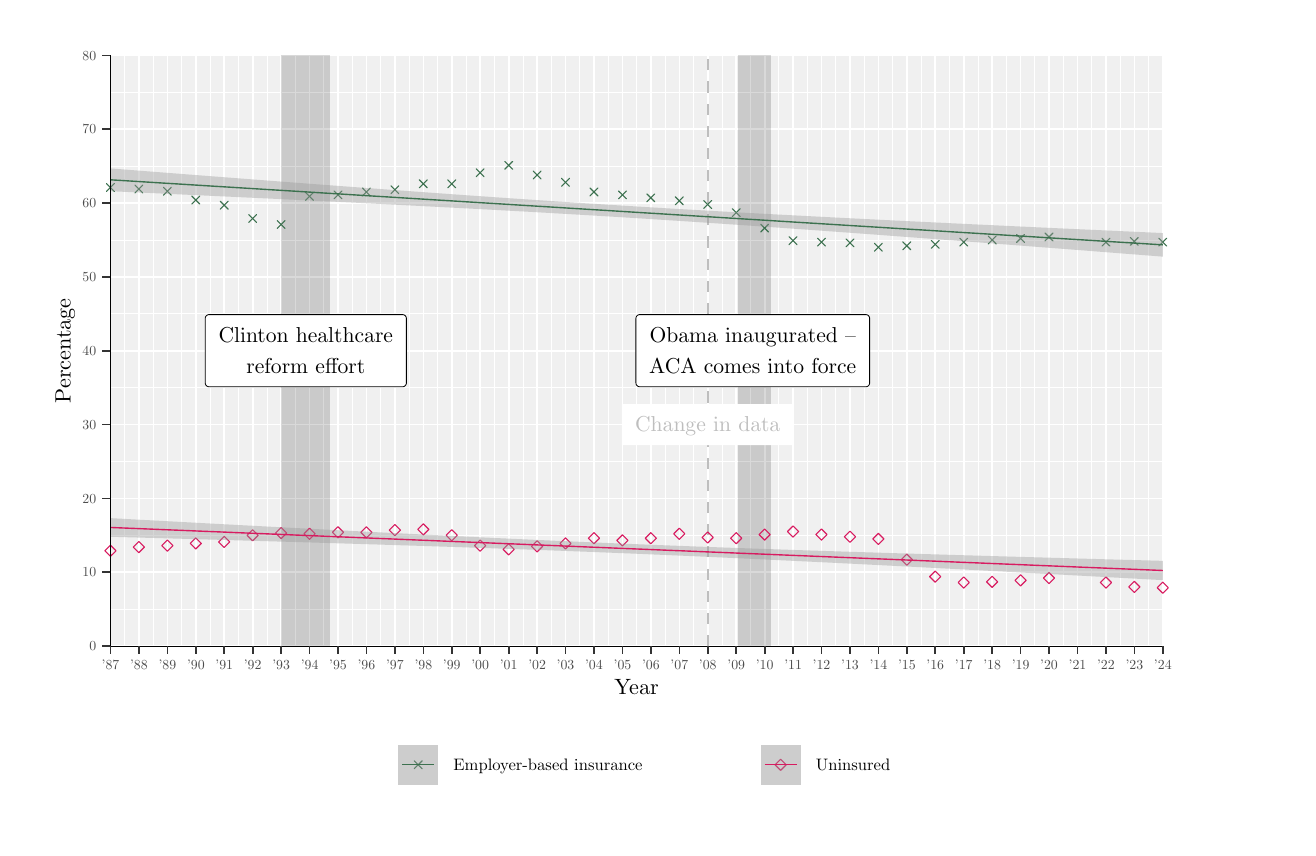
\begin{tikzpicture}[x=1pt,y=1pt]
\definecolor{fillColor}{RGB}{255,255,255}
\path[use as bounding box,fill=fillColor,fill opacity=0.00] (0,0) rectangle (455.30,289.08);
\begin{scope}
\path[clip] (  0.00,  0.00) rectangle (455.30,289.08);
\definecolor{drawColor}{RGB}{255,255,255}
\definecolor{fillColor}{RGB}{255,255,255}

\path[draw=drawColor,line width= 0.6pt,line join=round,line cap=round,fill=fillColor] ( -0.00,  0.00) rectangle (455.30,289.08);
\end{scope}
\begin{scope}
\path[clip] (  0.00,  0.00) rectangle (455.30,289.08);
\definecolor{fillColor}{gray}{0.94}

\path[fill=fillColor] ( 29.76, 65.63) rectangle (410.30,279.08);
\definecolor{drawColor}{RGB}{255,255,255}

\path[draw=drawColor,line width= 0.3pt,line join=round] ( 29.76, 78.97) --
	(410.30, 78.97);

\path[draw=drawColor,line width= 0.3pt,line join=round] ( 29.76,105.66) --
	(410.30,105.66);

\path[draw=drawColor,line width= 0.3pt,line join=round] ( 29.76,132.34) --
	(410.30,132.34);

\path[draw=drawColor,line width= 0.3pt,line join=round] ( 29.76,159.02) --
	(410.30,159.02);

\path[draw=drawColor,line width= 0.3pt,line join=round] ( 29.76,185.70) --
	(410.30,185.70);

\path[draw=drawColor,line width= 0.3pt,line join=round] ( 29.76,212.38) --
	(410.30,212.38);

\path[draw=drawColor,line width= 0.3pt,line join=round] ( 29.76,239.06) --
	(410.30,239.06);

\path[draw=drawColor,line width= 0.3pt,line join=round] ( 29.76,265.74) --
	(410.30,265.74);

\path[draw=drawColor,line width= 0.3pt,line join=round] ( 35.07, 65.63) --
	( 35.07,279.08);

\path[draw=drawColor,line width= 0.3pt,line join=round] ( 45.35, 65.63) --
	( 45.35,279.08);

\path[draw=drawColor,line width= 0.3pt,line join=round] ( 55.64, 65.63) --
	( 55.64,279.08);

\path[draw=drawColor,line width= 0.3pt,line join=round] ( 65.91, 65.63) --
	( 65.91,279.08);

\path[draw=drawColor,line width= 0.3pt,line join=round] ( 76.18, 65.63) --
	( 76.18,279.08);

\path[draw=drawColor,line width= 0.3pt,line join=round] ( 86.46, 65.63) --
	( 86.46,279.08);

\path[draw=drawColor,line width= 0.3pt,line join=round] ( 96.75, 65.63) --
	( 96.75,279.08);

\path[draw=drawColor,line width= 0.3pt,line join=round] (107.02, 65.63) --
	(107.02,279.08);

\path[draw=drawColor,line width= 0.3pt,line join=round] (117.29, 65.63) --
	(117.29,279.08);

\path[draw=drawColor,line width= 0.3pt,line join=round] (127.57, 65.63) --
	(127.57,279.08);

\path[draw=drawColor,line width= 0.3pt,line join=round] (137.86, 65.63) --
	(137.86,279.08);

\path[draw=drawColor,line width= 0.3pt,line join=round] (148.13, 65.63) --
	(148.13,279.08);

\path[draw=drawColor,line width= 0.3pt,line join=round] (158.40, 65.63) --
	(158.40,279.08);

\path[draw=drawColor,line width= 0.3pt,line join=round] (168.68, 65.63) --
	(168.68,279.08);

\path[draw=drawColor,line width= 0.3pt,line join=round] (178.97, 65.63) --
	(178.97,279.08);

\path[draw=drawColor,line width= 0.3pt,line join=round] (189.24, 65.63) --
	(189.24,279.08);

\path[draw=drawColor,line width= 0.3pt,line join=round] (199.51, 65.63) --
	(199.51,279.08);

\path[draw=drawColor,line width= 0.3pt,line join=round] (209.79, 65.63) --
	(209.79,279.08);

\path[draw=drawColor,line width= 0.3pt,line join=round] (220.07, 65.63) --
	(220.07,279.08);

\path[draw=drawColor,line width= 0.3pt,line join=round] (230.34, 65.63) --
	(230.34,279.08);

\path[draw=drawColor,line width= 0.3pt,line join=round] (240.62, 65.63) --
	(240.62,279.08);

\path[draw=drawColor,line width= 0.3pt,line join=round] (250.90, 65.63) --
	(250.90,279.08);

\path[draw=drawColor,line width= 0.3pt,line join=round] (261.18, 65.63) --
	(261.18,279.08);

\path[draw=drawColor,line width= 0.3pt,line join=round] (271.45, 65.63) --
	(271.45,279.08);

\path[draw=drawColor,line width= 0.3pt,line join=round] (281.72, 65.63) --
	(281.72,279.08);

\path[draw=drawColor,line width= 0.3pt,line join=round] (292.01, 65.63) --
	(292.01,279.08);

\path[draw=drawColor,line width= 0.3pt,line join=round] (302.29, 65.63) --
	(302.29,279.08);

\path[draw=drawColor,line width= 0.3pt,line join=round] (312.56, 65.63) --
	(312.56,279.08);

\path[draw=drawColor,line width= 0.3pt,line join=round] (322.83, 65.63) --
	(322.83,279.08);

\path[draw=drawColor,line width= 0.3pt,line join=round] (333.12, 65.63) --
	(333.12,279.08);

\path[draw=drawColor,line width= 0.3pt,line join=round] (343.40, 65.63) --
	(343.40,279.08);

\path[draw=drawColor,line width= 0.3pt,line join=round] (353.67, 65.63) --
	(353.67,279.08);

\path[draw=drawColor,line width= 0.3pt,line join=round] (363.94, 65.63) --
	(363.94,279.08);

\path[draw=drawColor,line width= 0.3pt,line join=round] (374.23, 65.63) --
	(374.23,279.08);

\path[draw=drawColor,line width= 0.3pt,line join=round] (384.51, 65.63) --
	(384.51,279.08);

\path[draw=drawColor,line width= 0.3pt,line join=round] (394.78, 65.63) --
	(394.78,279.08);

\path[draw=drawColor,line width= 0.3pt,line join=round] (405.05, 65.63) --
	(405.05,279.08);

\path[draw=drawColor,line width= 0.6pt,line join=round] ( 29.76, 65.63) --
	(410.30, 65.63);

\path[draw=drawColor,line width= 0.6pt,line join=round] ( 29.76, 92.32) --
	(410.30, 92.32);

\path[draw=drawColor,line width= 0.6pt,line join=round] ( 29.76,119.00) --
	(410.30,119.00);

\path[draw=drawColor,line width= 0.6pt,line join=round] ( 29.76,145.68) --
	(410.30,145.68);

\path[draw=drawColor,line width= 0.6pt,line join=round] ( 29.76,172.36) --
	(410.30,172.36);

\path[draw=drawColor,line width= 0.6pt,line join=round] ( 29.76,199.04) --
	(410.30,199.04);

\path[draw=drawColor,line width= 0.6pt,line join=round] ( 29.76,225.72) --
	(410.30,225.72);

\path[draw=drawColor,line width= 0.6pt,line join=round] ( 29.76,252.40) --
	(410.30,252.40);

\path[draw=drawColor,line width= 0.6pt,line join=round] ( 29.76,279.08) --
	(410.30,279.08);

\path[draw=drawColor,line width= 0.6pt,line join=round] ( 29.93, 65.63) --
	( 29.93,279.08);

\path[draw=drawColor,line width= 0.6pt,line join=round] ( 40.20, 65.63) --
	( 40.20,279.08);

\path[draw=drawColor,line width= 0.6pt,line join=round] ( 50.50, 65.63) --
	( 50.50,279.08);

\path[draw=drawColor,line width= 0.6pt,line join=round] ( 60.77, 65.63) --
	( 60.77,279.08);

\path[draw=drawColor,line width= 0.6pt,line join=round] ( 71.04, 65.63) --
	( 71.04,279.08);

\path[draw=drawColor,line width= 0.6pt,line join=round] ( 81.31, 65.63) --
	( 81.31,279.08);

\path[draw=drawColor,line width= 0.6pt,line join=round] ( 91.61, 65.63) --
	( 91.61,279.08);

\path[draw=drawColor,line width= 0.6pt,line join=round] (101.88, 65.63) --
	(101.88,279.08);

\path[draw=drawColor,line width= 0.6pt,line join=round] (112.15, 65.63) --
	(112.15,279.08);

\path[draw=drawColor,line width= 0.6pt,line join=round] (122.42, 65.63) --
	(122.42,279.08);

\path[draw=drawColor,line width= 0.6pt,line join=round] (132.72, 65.63) --
	(132.72,279.08);

\path[draw=drawColor,line width= 0.6pt,line join=round] (142.99, 65.63) --
	(142.99,279.08);

\path[draw=drawColor,line width= 0.6pt,line join=round] (153.26, 65.63) --
	(153.26,279.08);

\path[draw=drawColor,line width= 0.6pt,line join=round] (163.53, 65.63) --
	(163.53,279.08);

\path[draw=drawColor,line width= 0.6pt,line join=round] (173.83, 65.63) --
	(173.83,279.08);

\path[draw=drawColor,line width= 0.6pt,line join=round] (184.10, 65.63) --
	(184.10,279.08);

\path[draw=drawColor,line width= 0.6pt,line join=round] (194.37, 65.63) --
	(194.37,279.08);

\path[draw=drawColor,line width= 0.6pt,line join=round] (204.64, 65.63) --
	(204.64,279.08);

\path[draw=drawColor,line width= 0.6pt,line join=round] (214.94, 65.63) --
	(214.94,279.08);

\path[draw=drawColor,line width= 0.6pt,line join=round] (225.21, 65.63) --
	(225.21,279.08);

\path[draw=drawColor,line width= 0.6pt,line join=round] (235.48, 65.63) --
	(235.48,279.08);

\path[draw=drawColor,line width= 0.6pt,line join=round] (245.75, 65.63) --
	(245.75,279.08);

\path[draw=drawColor,line width= 0.6pt,line join=round] (256.05, 65.63) --
	(256.05,279.08);

\path[draw=drawColor,line width= 0.6pt,line join=round] (266.32, 65.63) --
	(266.32,279.08);

\path[draw=drawColor,line width= 0.6pt,line join=round] (276.59, 65.63) --
	(276.59,279.08);

\path[draw=drawColor,line width= 0.6pt,line join=round] (286.86, 65.63) --
	(286.86,279.08);

\path[draw=drawColor,line width= 0.6pt,line join=round] (297.16, 65.63) --
	(297.16,279.08);

\path[draw=drawColor,line width= 0.6pt,line join=round] (307.43, 65.63) --
	(307.43,279.08);

\path[draw=drawColor,line width= 0.6pt,line join=round] (317.70, 65.63) --
	(317.70,279.08);

\path[draw=drawColor,line width= 0.6pt,line join=round] (327.97, 65.63) --
	(327.97,279.08);

\path[draw=drawColor,line width= 0.6pt,line join=round] (338.27, 65.63) --
	(338.27,279.08);

\path[draw=drawColor,line width= 0.6pt,line join=round] (348.54, 65.63) --
	(348.54,279.08);

\path[draw=drawColor,line width= 0.6pt,line join=round] (358.81, 65.63) --
	(358.81,279.08);

\path[draw=drawColor,line width= 0.6pt,line join=round] (369.08, 65.63) --
	(369.08,279.08);

\path[draw=drawColor,line width= 0.6pt,line join=round] (379.38, 65.63) --
	(379.38,279.08);

\path[draw=drawColor,line width= 0.6pt,line join=round] (389.65, 65.63) --
	(389.65,279.08);

\path[draw=drawColor,line width= 0.6pt,line join=round] (399.92, 65.63) --
	(399.92,279.08);

\path[draw=drawColor,line width= 0.6pt,line join=round] (410.19, 65.63) --
	(410.19,279.08);
\definecolor{fillColor}{RGB}{190,190,190}

\path[fill=fillColor,fill opacity=0.01] ( 91.61, 65.63) rectangle (109.42,279.08);

\path[fill=fillColor,fill opacity=0.01] ( 91.61, 65.63) rectangle (109.42,279.08);

\path[fill=fillColor,fill opacity=0.01] ( 91.61, 65.63) rectangle (109.42,279.08);

\path[fill=fillColor,fill opacity=0.01] ( 91.61, 65.63) rectangle (109.42,279.08);

\path[fill=fillColor,fill opacity=0.01] ( 91.61, 65.63) rectangle (109.42,279.08);

\path[fill=fillColor,fill opacity=0.01] ( 91.61, 65.63) rectangle (109.42,279.08);

\path[fill=fillColor,fill opacity=0.01] ( 91.61, 65.63) rectangle (109.42,279.08);

\path[fill=fillColor,fill opacity=0.01] ( 91.61, 65.63) rectangle (109.42,279.08);

\path[fill=fillColor,fill opacity=0.01] ( 91.61, 65.63) rectangle (109.42,279.08);

\path[fill=fillColor,fill opacity=0.01] ( 91.61, 65.63) rectangle (109.42,279.08);

\path[fill=fillColor,fill opacity=0.01] ( 91.61, 65.63) rectangle (109.42,279.08);

\path[fill=fillColor,fill opacity=0.01] ( 91.61, 65.63) rectangle (109.42,279.08);

\path[fill=fillColor,fill opacity=0.01] ( 91.61, 65.63) rectangle (109.42,279.08);

\path[fill=fillColor,fill opacity=0.01] ( 91.61, 65.63) rectangle (109.42,279.08);

\path[fill=fillColor,fill opacity=0.01] ( 91.61, 65.63) rectangle (109.42,279.08);

\path[fill=fillColor,fill opacity=0.01] ( 91.61, 65.63) rectangle (109.42,279.08);

\path[fill=fillColor,fill opacity=0.01] ( 91.61, 65.63) rectangle (109.42,279.08);

\path[fill=fillColor,fill opacity=0.01] ( 91.61, 65.63) rectangle (109.42,279.08);

\path[fill=fillColor,fill opacity=0.01] ( 91.61, 65.63) rectangle (109.42,279.08);

\path[fill=fillColor,fill opacity=0.01] ( 91.61, 65.63) rectangle (109.42,279.08);

\path[fill=fillColor,fill opacity=0.01] ( 91.61, 65.63) rectangle (109.42,279.08);

\path[fill=fillColor,fill opacity=0.01] ( 91.61, 65.63) rectangle (109.42,279.08);

\path[fill=fillColor,fill opacity=0.01] ( 91.61, 65.63) rectangle (109.42,279.08);

\path[fill=fillColor,fill opacity=0.01] ( 91.61, 65.63) rectangle (109.42,279.08);

\path[fill=fillColor,fill opacity=0.01] ( 91.61, 65.63) rectangle (109.42,279.08);

\path[fill=fillColor,fill opacity=0.01] ( 91.61, 65.63) rectangle (109.42,279.08);

\path[fill=fillColor,fill opacity=0.01] ( 91.61, 65.63) rectangle (109.42,279.08);

\path[fill=fillColor,fill opacity=0.01] ( 91.61, 65.63) rectangle (109.42,279.08);

\path[fill=fillColor,fill opacity=0.01] ( 91.61, 65.63) rectangle (109.42,279.08);

\path[fill=fillColor,fill opacity=0.01] ( 91.61, 65.63) rectangle (109.42,279.08);

\path[fill=fillColor,fill opacity=0.01] ( 91.61, 65.63) rectangle (109.42,279.08);

\path[fill=fillColor,fill opacity=0.01] ( 91.61, 65.63) rectangle (109.42,279.08);

\path[fill=fillColor,fill opacity=0.01] ( 91.61, 65.63) rectangle (109.42,279.08);

\path[fill=fillColor,fill opacity=0.01] ( 91.61, 65.63) rectangle (109.42,279.08);

\path[fill=fillColor,fill opacity=0.01] ( 91.61, 65.63) rectangle (109.42,279.08);

\path[fill=fillColor,fill opacity=0.01] ( 91.61, 65.63) rectangle (109.42,279.08);

\path[fill=fillColor,fill opacity=0.01] ( 91.61, 65.63) rectangle (109.42,279.08);

\path[fill=fillColor,fill opacity=0.01] ( 91.61, 65.63) rectangle (109.42,279.08);

\path[fill=fillColor,fill opacity=0.01] (256.58, 65.63) rectangle (268.60,279.08);

\path[fill=fillColor,fill opacity=0.01] (256.58, 65.63) rectangle (268.60,279.08);

\path[fill=fillColor,fill opacity=0.01] (256.58, 65.63) rectangle (268.60,279.08);

\path[fill=fillColor,fill opacity=0.01] (256.58, 65.63) rectangle (268.60,279.08);

\path[fill=fillColor,fill opacity=0.01] (256.58, 65.63) rectangle (268.60,279.08);

\path[fill=fillColor,fill opacity=0.01] (256.58, 65.63) rectangle (268.60,279.08);

\path[fill=fillColor,fill opacity=0.01] (256.58, 65.63) rectangle (268.60,279.08);

\path[fill=fillColor,fill opacity=0.01] (256.58, 65.63) rectangle (268.60,279.08);

\path[fill=fillColor,fill opacity=0.01] (256.58, 65.63) rectangle (268.60,279.08);

\path[fill=fillColor,fill opacity=0.01] (256.58, 65.63) rectangle (268.60,279.08);

\path[fill=fillColor,fill opacity=0.01] (256.58, 65.63) rectangle (268.60,279.08);

\path[fill=fillColor,fill opacity=0.01] (256.58, 65.63) rectangle (268.60,279.08);

\path[fill=fillColor,fill opacity=0.01] (256.58, 65.63) rectangle (268.60,279.08);

\path[fill=fillColor,fill opacity=0.01] (256.58, 65.63) rectangle (268.60,279.08);

\path[fill=fillColor,fill opacity=0.01] (256.58, 65.63) rectangle (268.60,279.08);

\path[fill=fillColor,fill opacity=0.01] (256.58, 65.63) rectangle (268.60,279.08);

\path[fill=fillColor,fill opacity=0.01] (256.58, 65.63) rectangle (268.60,279.08);

\path[fill=fillColor,fill opacity=0.01] (256.58, 65.63) rectangle (268.60,279.08);

\path[fill=fillColor,fill opacity=0.01] (256.58, 65.63) rectangle (268.60,279.08);

\path[fill=fillColor,fill opacity=0.01] (256.58, 65.63) rectangle (268.60,279.08);

\path[fill=fillColor,fill opacity=0.01] (256.58, 65.63) rectangle (268.60,279.08);

\path[fill=fillColor,fill opacity=0.01] (256.58, 65.63) rectangle (268.60,279.08);

\path[fill=fillColor,fill opacity=0.01] (256.58, 65.63) rectangle (268.60,279.08);

\path[fill=fillColor,fill opacity=0.01] (256.58, 65.63) rectangle (268.60,279.08);

\path[fill=fillColor,fill opacity=0.01] (256.58, 65.63) rectangle (268.60,279.08);

\path[fill=fillColor,fill opacity=0.01] (256.58, 65.63) rectangle (268.60,279.08);

\path[fill=fillColor,fill opacity=0.01] (256.58, 65.63) rectangle (268.60,279.08);

\path[fill=fillColor,fill opacity=0.01] (256.58, 65.63) rectangle (268.60,279.08);

\path[fill=fillColor,fill opacity=0.01] (256.58, 65.63) rectangle (268.60,279.08);

\path[fill=fillColor,fill opacity=0.01] (256.58, 65.63) rectangle (268.60,279.08);

\path[fill=fillColor,fill opacity=0.01] (256.58, 65.63) rectangle (268.60,279.08);

\path[fill=fillColor,fill opacity=0.01] (256.58, 65.63) rectangle (268.60,279.08);

\path[fill=fillColor,fill opacity=0.01] (256.58, 65.63) rectangle (268.60,279.08);

\path[fill=fillColor,fill opacity=0.01] (256.58, 65.63) rectangle (268.60,279.08);

\path[fill=fillColor,fill opacity=0.01] (256.58, 65.63) rectangle (268.60,279.08);

\path[fill=fillColor,fill opacity=0.01] (256.58, 65.63) rectangle (268.60,279.08);

\path[fill=fillColor,fill opacity=0.01] (256.58, 65.63) rectangle (268.60,279.08);

\path[fill=fillColor,fill opacity=0.01] (256.58, 65.63) rectangle (268.60,279.08);
\definecolor{drawColor}{RGB}{190,190,190}

\path[draw=drawColor,line width= 0.6pt,dash pattern=on 4pt off 4pt ,line join=round] (245.72, 65.63) -- (245.72,279.08);
\definecolor{drawColor}{RGB}{60,113,79}

\path[draw=drawColor,line width= 0.4pt,line join=round,line cap=round] ( 28.48,229.89) -- ( 31.33,232.75);

\path[draw=drawColor,line width= 0.4pt,line join=round,line cap=round] ( 28.48,232.75) -- ( 31.33,229.89);

\path[draw=drawColor,line width= 0.4pt,line join=round,line cap=round] ( 38.75,229.36) -- ( 41.60,232.21);

\path[draw=drawColor,line width= 0.4pt,line join=round,line cap=round] ( 38.75,232.21) -- ( 41.60,229.36);

\path[draw=drawColor,line width= 0.4pt,line join=round,line cap=round] ( 49.05,228.56) -- ( 51.90,231.41);

\path[draw=drawColor,line width= 0.4pt,line join=round,line cap=round] ( 49.05,231.41) -- ( 51.90,228.56);

\path[draw=drawColor,line width= 0.4pt,line join=round,line cap=round] ( 59.32,225.36) -- ( 62.17,228.21);

\path[draw=drawColor,line width= 0.4pt,line join=round,line cap=round] ( 59.32,228.21) -- ( 62.17,225.36);

\path[draw=drawColor,line width= 0.4pt,line join=round,line cap=round] ( 69.59,223.49) -- ( 72.44,226.34);

\path[draw=drawColor,line width= 0.4pt,line join=round,line cap=round] ( 69.59,226.34) -- ( 72.44,223.49);

\path[draw=drawColor,line width= 0.4pt,line join=round,line cap=round] ( 79.86,218.69) -- ( 82.71,221.54);

\path[draw=drawColor,line width= 0.4pt,line join=round,line cap=round] ( 79.86,221.54) -- ( 82.71,218.69);

\path[draw=drawColor,line width= 0.4pt,line join=round,line cap=round] ( 90.16,216.55) -- ( 93.01,219.41);

\path[draw=drawColor,line width= 0.4pt,line join=round,line cap=round] ( 90.16,219.41) -- ( 93.01,216.55);

\path[draw=drawColor,line width= 0.4pt,line join=round,line cap=round] (100.43,226.69) -- (103.28,229.55);

\path[draw=drawColor,line width= 0.4pt,line join=round,line cap=round] (100.43,229.55) -- (103.28,226.69);

\path[draw=drawColor,line width= 0.4pt,line join=round,line cap=round] (110.70,227.23) -- (113.55,230.08);

\path[draw=drawColor,line width= 0.4pt,line join=round,line cap=round] (110.70,230.08) -- (113.55,227.23);

\path[draw=drawColor,line width= 0.4pt,line join=round,line cap=round] (120.97,228.29) -- (123.82,231.15);

\path[draw=drawColor,line width= 0.4pt,line join=round,line cap=round] (120.97,231.15) -- (123.82,228.29);

\path[draw=drawColor,line width= 0.4pt,line join=round,line cap=round] (131.27,229.09) -- (134.12,231.95);

\path[draw=drawColor,line width= 0.4pt,line join=round,line cap=round] (131.27,231.95) -- (134.12,229.09);

\path[draw=drawColor,line width= 0.4pt,line join=round,line cap=round] (141.54,231.23) -- (144.39,234.08);

\path[draw=drawColor,line width= 0.4pt,line join=round,line cap=round] (141.54,234.08) -- (144.39,231.23);

\path[draw=drawColor,line width= 0.4pt,line join=round,line cap=round] (151.81,231.23) -- (154.66,234.08);

\path[draw=drawColor,line width= 0.4pt,line join=round,line cap=round] (151.81,234.08) -- (154.66,231.23);

\path[draw=drawColor,line width= 0.4pt,line join=round,line cap=round] (162.08,235.23) -- (164.93,238.08);

\path[draw=drawColor,line width= 0.4pt,line join=round,line cap=round] (162.08,238.08) -- (164.93,235.23);

\path[draw=drawColor,line width= 0.4pt,line join=round,line cap=round] (172.38,237.90) -- (175.23,240.75);

\path[draw=drawColor,line width= 0.4pt,line join=round,line cap=round] (172.38,240.75) -- (175.23,237.90);

\path[draw=drawColor,line width= 0.4pt,line join=round,line cap=round] (182.65,234.43) -- (185.50,237.28);

\path[draw=drawColor,line width= 0.4pt,line join=round,line cap=round] (182.65,237.28) -- (185.50,234.43);

\path[draw=drawColor,line width= 0.4pt,line join=round,line cap=round] (192.92,231.76) -- (195.77,234.62);

\path[draw=drawColor,line width= 0.4pt,line join=round,line cap=round] (192.92,234.62) -- (195.77,231.76);

\path[draw=drawColor,line width= 0.4pt,line join=round,line cap=round] (203.19,228.29) -- (206.04,231.15);

\path[draw=drawColor,line width= 0.4pt,line join=round,line cap=round] (203.19,231.15) -- (206.04,228.29);

\path[draw=drawColor,line width= 0.4pt,line join=round,line cap=round] (213.48,227.23) -- (216.34,230.08);

\path[draw=drawColor,line width= 0.4pt,line join=round,line cap=round] (213.48,230.08) -- (216.34,227.23);

\path[draw=drawColor,line width= 0.4pt,line join=round,line cap=round] (223.75,226.16) -- (226.61,229.01);

\path[draw=drawColor,line width= 0.4pt,line join=round,line cap=round] (223.75,229.01) -- (226.61,226.16);

\path[draw=drawColor,line width= 0.4pt,line join=round,line cap=round] (234.03,225.09) -- (236.88,227.95);

\path[draw=drawColor,line width= 0.4pt,line join=round,line cap=round] (234.03,227.95) -- (236.88,225.09);

\path[draw=drawColor,line width= 0.4pt,line join=round,line cap=round] (244.30,223.76) -- (247.15,226.61);

\path[draw=drawColor,line width= 0.4pt,line join=round,line cap=round] (244.30,226.61) -- (247.15,223.76);

\path[draw=drawColor,line width= 0.4pt,line join=round,line cap=round] (254.59,220.82) -- (257.45,223.68);

\path[draw=drawColor,line width= 0.4pt,line join=round,line cap=round] (254.59,223.68) -- (257.45,220.82);

\path[draw=drawColor,line width= 0.4pt,line join=round,line cap=round] (264.86,215.22) -- (267.72,218.07);

\path[draw=drawColor,line width= 0.4pt,line join=round,line cap=round] (264.86,218.07) -- (267.72,215.22);

\path[draw=drawColor,line width= 0.4pt,line join=round,line cap=round] (275.13,210.68) -- (277.99,213.54);

\path[draw=drawColor,line width= 0.4pt,line join=round,line cap=round] (275.13,213.54) -- (277.99,210.68);

\path[draw=drawColor,line width= 0.4pt,line join=round,line cap=round] (285.41,210.15) -- (288.26,213.00);

\path[draw=drawColor,line width= 0.4pt,line join=round,line cap=round] (285.41,213.00) -- (288.26,210.15);

\path[draw=drawColor,line width= 0.4pt,line join=round,line cap=round] (295.70,209.88) -- (298.56,212.74);

\path[draw=drawColor,line width= 0.4pt,line join=round,line cap=round] (295.70,212.74) -- (298.56,209.88);

\path[draw=drawColor,line width= 0.4pt,line join=round,line cap=round] (305.97,208.28) -- (308.83,211.14);

\path[draw=drawColor,line width= 0.4pt,line join=round,line cap=round] (305.97,211.14) -- (308.83,208.28);

\path[draw=drawColor,line width= 0.4pt,line join=round,line cap=round] (316.24,208.82) -- (319.10,211.67);

\path[draw=drawColor,line width= 0.4pt,line join=round,line cap=round] (316.24,211.67) -- (319.10,208.82);

\path[draw=drawColor,line width= 0.4pt,line join=round,line cap=round] (326.51,209.35) -- (329.37,212.20);

\path[draw=drawColor,line width= 0.4pt,line join=round,line cap=round] (326.51,212.20) -- (329.37,209.35);

\path[draw=drawColor,line width= 0.4pt,line join=round,line cap=round] (336.81,210.15) -- (339.67,213.00);

\path[draw=drawColor,line width= 0.4pt,line join=round,line cap=round] (336.81,213.00) -- (339.67,210.15);

\path[draw=drawColor,line width= 0.4pt,line join=round,line cap=round] (347.08,210.95) -- (349.94,213.80);

\path[draw=drawColor,line width= 0.4pt,line join=round,line cap=round] (347.08,213.80) -- (349.94,210.95);

\path[draw=drawColor,line width= 0.4pt,line join=round,line cap=round] (357.35,211.49) -- (360.21,214.34);

\path[draw=drawColor,line width= 0.4pt,line join=round,line cap=round] (357.35,214.34) -- (360.21,211.49);

\path[draw=drawColor,line width= 0.4pt,line join=round,line cap=round] (367.62,212.02) -- (370.48,214.87);

\path[draw=drawColor,line width= 0.4pt,line join=round,line cap=round] (367.62,214.87) -- (370.48,212.02);

\path[draw=drawColor,line width= 0.4pt,line join=round,line cap=round] (388.19,210.15) -- (391.05,213.00);

\path[draw=drawColor,line width= 0.4pt,line join=round,line cap=round] (388.19,213.00) -- (391.05,210.15);

\path[draw=drawColor,line width= 0.4pt,line join=round,line cap=round] (398.46,210.42) -- (401.32,213.27);

\path[draw=drawColor,line width= 0.4pt,line join=round,line cap=round] (398.46,213.27) -- (401.32,210.42);

\path[draw=drawColor,line width= 0.4pt,line join=round,line cap=round] (408.73,210.15) -- (411.59,213.00);

\path[draw=drawColor,line width= 0.4pt,line join=round,line cap=round] (408.73,213.00) -- (411.59,210.15);
\definecolor{drawColor}{RGB}{216,27,96}

\path[draw=drawColor,line width= 0.4pt,line join=round,line cap=round] ( 27.89,100.05) --
	( 29.90,102.07) --
	( 31.92,100.05) --
	( 29.90, 98.04) --
	cycle;

\path[draw=drawColor,line width= 0.4pt,line join=round,line cap=round] ( 38.16,101.39) --
	( 40.17,103.40) --
	( 42.19,101.39) --
	( 40.17, 99.37) --
	cycle;

\path[draw=drawColor,line width= 0.4pt,line join=round,line cap=round] ( 48.46,101.92) --
	( 50.47,103.94) --
	( 52.49,101.92) --
	( 50.47, 99.90) --
	cycle;

\path[draw=drawColor,line width= 0.4pt,line join=round,line cap=round] ( 58.73,102.72) --
	( 60.74,104.74) --
	( 62.76,102.72) --
	( 60.74,100.70) --
	cycle;

\path[draw=drawColor,line width= 0.4pt,line join=round,line cap=round] ( 69.00,103.25) --
	( 71.01,105.27) --
	( 73.03,103.25) --
	( 71.01,101.24) --
	cycle;

\path[draw=drawColor,line width= 0.4pt,line join=round,line cap=round] ( 79.27,105.66) --
	( 81.28,107.67) --
	( 83.30,105.66) --
	( 81.28,103.64) --
	cycle;

\path[draw=drawColor,line width= 0.4pt,line join=round,line cap=round] ( 89.57,106.46) --
	( 91.58,108.47) --
	( 93.60,106.46) --
	( 91.58,104.44) --
	cycle;

\path[draw=drawColor,line width= 0.4pt,line join=round,line cap=round] ( 99.84,106.19) --
	(101.85,108.21) --
	(103.87,106.19) --
	(101.85,104.17) --
	cycle;

\path[draw=drawColor,line width= 0.4pt,line join=round,line cap=round] (110.11,106.72) --
	(112.12,108.74) --
	(114.14,106.72) --
	(112.12,104.71) --
	cycle;

\path[draw=drawColor,line width= 0.4pt,line join=round,line cap=round] (120.38,106.72) --
	(122.39,108.74) --
	(124.41,106.72) --
	(122.39,104.71) --
	cycle;

\path[draw=drawColor,line width= 0.4pt,line join=round,line cap=round] (130.67,107.52) --
	(132.69,109.54) --
	(134.71,107.52) --
	(132.69,105.51) --
	cycle;

\path[draw=drawColor,line width= 0.4pt,line join=round,line cap=round] (140.95,107.79) --
	(142.96,109.81) --
	(144.98,107.79) --
	(142.96,105.77) --
	cycle;

\path[draw=drawColor,line width= 0.4pt,line join=round,line cap=round] (151.22,105.66) --
	(153.23,107.67) --
	(155.25,105.66) --
	(153.23,103.64) --
	cycle;

\path[draw=drawColor,line width= 0.4pt,line join=round,line cap=round] (161.49,101.92) --
	(163.50,103.94) --
	(165.52,101.92) --
	(163.50, 99.90) --
	cycle;

\path[draw=drawColor,line width= 0.4pt,line join=round,line cap=round] (171.78,100.59) --
	(173.80,102.60) --
	(175.82,100.59) --
	(173.80, 98.57) --
	cycle;

\path[draw=drawColor,line width= 0.4pt,line join=round,line cap=round] (182.05,101.65) --
	(184.07,103.67) --
	(186.09,101.65) --
	(184.07, 99.64) --
	cycle;

\path[draw=drawColor,line width= 0.4pt,line join=round,line cap=round] (192.32,102.72) --
	(194.34,104.74) --
	(196.36,102.72) --
	(194.34,100.70) --
	cycle;

\path[draw=drawColor,line width= 0.4pt,line join=round,line cap=round] (202.60,104.59) --
	(204.61,106.61) --
	(206.63,104.59) --
	(204.61,102.57) --
	cycle;

\path[draw=drawColor,line width= 0.4pt,line join=round,line cap=round] (212.89,103.79) --
	(214.91,105.81) --
	(216.93,103.79) --
	(214.91,101.77) --
	cycle;

\path[draw=drawColor,line width= 0.4pt,line join=round,line cap=round] (223.16,104.59) --
	(225.18,106.61) --
	(227.20,104.59) --
	(225.18,102.57) --
	cycle;

\path[draw=drawColor,line width= 0.4pt,line join=round,line cap=round] (233.43,106.19) --
	(235.45,108.21) --
	(237.47,106.19) --
	(235.45,104.17) --
	cycle;

\path[draw=drawColor,line width= 0.4pt,line join=round,line cap=round] (243.70,104.86) --
	(245.72,106.87) --
	(247.74,104.86) --
	(245.72,102.84) --
	cycle;

\path[draw=drawColor,line width= 0.4pt,line join=round,line cap=round] (254.00,104.59) --
	(256.02,106.61) --
	(258.04,104.59) --
	(256.02,102.57) --
	cycle;

\path[draw=drawColor,line width= 0.4pt,line join=round,line cap=round] (264.27,105.92) --
	(266.29,107.94) --
	(268.31,105.92) --
	(266.29,103.90) --
	cycle;

\path[draw=drawColor,line width= 0.4pt,line join=round,line cap=round] (274.54,106.99) --
	(276.56,109.01) --
	(278.58,106.99) --
	(276.56,104.97) --
	cycle;

\path[draw=drawColor,line width= 0.4pt,line join=round,line cap=round] (284.81,105.92) --
	(286.83,107.94) --
	(288.85,105.92) --
	(286.83,103.90) --
	cycle;

\path[draw=drawColor,line width= 0.4pt,line join=round,line cap=round] (295.11,105.12) --
	(297.13,107.14) --
	(299.15,105.12) --
	(297.13,103.10) --
	cycle;

\path[draw=drawColor,line width= 0.4pt,line join=round,line cap=round] (305.38,104.32) --
	(307.40,106.34) --
	(309.42,104.32) --
	(307.40,102.30) --
	cycle;

\path[draw=drawColor,line width= 0.4pt,line join=round,line cap=round] (315.65, 96.85) --
	(317.67, 98.87) --
	(319.69, 96.85) --
	(317.67, 94.83) --
	cycle;

\path[draw=drawColor,line width= 0.4pt,line join=round,line cap=round] (325.92, 90.71) --
	(327.94, 92.73) --
	(329.96, 90.71) --
	(327.94, 88.70) --
	cycle;

\path[draw=drawColor,line width= 0.4pt,line join=round,line cap=round] (336.22, 88.58) --
	(338.24, 90.60) --
	(340.26, 88.58) --
	(338.24, 86.56) --
	cycle;

\path[draw=drawColor,line width= 0.4pt,line join=round,line cap=round] (346.49, 88.85) --
	(348.51, 90.86) --
	(350.53, 88.85) --
	(348.51, 86.83) --
	cycle;

\path[draw=drawColor,line width= 0.4pt,line join=round,line cap=round] (356.76, 89.38) --
	(358.78, 91.40) --
	(360.80, 89.38) --
	(358.78, 87.36) --
	cycle;

\path[draw=drawColor,line width= 0.4pt,line join=round,line cap=round] (367.03, 90.18) --
	(369.05, 92.20) --
	(371.07, 90.18) --
	(369.05, 88.16) --
	cycle;

\path[draw=drawColor,line width= 0.4pt,line join=round,line cap=round] (387.60, 88.58) --
	(389.62, 90.60) --
	(391.64, 88.58) --
	(389.62, 86.56) --
	cycle;

\path[draw=drawColor,line width= 0.4pt,line join=round,line cap=round] (397.87, 86.98) --
	(399.89, 89.00) --
	(401.91, 86.98) --
	(399.89, 84.96) --
	cycle;

\path[draw=drawColor,line width= 0.4pt,line join=round,line cap=round] (408.14, 86.71) --
	(410.16, 88.73) --
	(412.18, 86.71) --
	(410.16, 84.69) --
	cycle;
\definecolor{fillColor}{RGB}{153,153,153}

\path[fill=fillColor,fill opacity=0.40] ( 29.90,238.22) --
	( 34.72,237.84) --
	( 39.53,237.47) --
	( 44.34,237.09) --
	( 49.16,236.72) --
	( 53.97,236.35) --
	( 58.78,235.97) --
	( 63.60,235.60) --
	( 68.41,235.23) --
	( 73.22,234.86) --
	( 78.04,234.49) --
	( 82.85,234.12) --
	( 87.66,233.76) --
	( 92.48,233.39) --
	( 97.29,233.03) --
	(102.10,232.66) --
	(106.92,232.30) --
	(111.73,231.94) --
	(116.55,231.58) --
	(121.36,231.22) --
	(126.17,230.87) --
	(130.99,230.51) --
	(135.80,230.16) --
	(140.61,229.81) --
	(145.43,229.46) --
	(150.24,229.12) --
	(155.05,228.77) --
	(159.87,228.43) --
	(164.68,228.10) --
	(169.49,227.76) --
	(174.31,227.43) --
	(179.12,227.10) --
	(183.93,226.78) --
	(188.75,226.46) --
	(193.56,226.14) --
	(198.37,225.83) --
	(203.19,225.52) --
	(208.00,225.21) --
	(212.81,224.91) --
	(217.63,224.61) --
	(222.44,224.32) --
	(227.25,224.03) --
	(232.07,223.74) --
	(236.88,223.46) --
	(241.69,223.18) --
	(246.51,222.91) --
	(251.32,222.64) --
	(256.13,222.37) --
	(260.95,222.10) --
	(265.76,221.84) --
	(270.57,221.58) --
	(275.39,221.33) --
	(280.20,221.08) --
	(285.01,220.83) --
	(289.83,220.58) --
	(294.64,220.33) --
	(299.45,220.09) --
	(304.27,219.85) --
	(309.08,219.61) --
	(313.89,219.37) --
	(318.71,219.13) --
	(323.52,218.90) --
	(328.33,218.67) --
	(333.15,218.43) --
	(337.96,218.20) --
	(342.77,217.97) --
	(347.59,217.75) --
	(352.40,217.52) --
	(357.21,217.29) --
	(362.03,217.07) --
	(366.84,216.84) --
	(371.65,216.62) --
	(376.47,216.40) --
	(381.28,216.18) --
	(386.09,215.96) --
	(390.91,215.74) --
	(395.72,215.52) --
	(400.53,215.30) --
	(405.35,215.08) --
	(410.16,214.86) --
	(410.16,206.34) --
	(405.35,206.72) --
	(400.53,207.10) --
	(395.72,207.47) --
	(390.91,207.85) --
	(386.09,208.22) --
	(381.28,208.60) --
	(376.47,208.97) --
	(371.65,209.34) --
	(366.84,209.71) --
	(362.03,210.08) --
	(357.21,210.45) --
	(352.40,210.82) --
	(347.59,211.19) --
	(342.77,211.56) --
	(337.96,211.92) --
	(333.15,212.29) --
	(328.33,212.65) --
	(323.52,213.01) --
	(318.71,213.37) --
	(313.89,213.73) --
	(309.08,214.09) --
	(304.27,214.45) --
	(299.45,214.80) --
	(294.64,215.15) --
	(289.83,215.50) --
	(285.01,215.85) --
	(280.20,216.19) --
	(275.39,216.53) --
	(270.57,216.87) --
	(265.76,217.21) --
	(260.95,217.54) --
	(256.13,217.87) --
	(251.32,218.20) --
	(246.51,218.52) --
	(241.69,218.84) --
	(236.88,219.16) --
	(232.07,219.47) --
	(227.25,219.78) --
	(222.44,220.09) --
	(217.63,220.39) --
	(212.81,220.69) --
	(208.00,220.98) --
	(203.19,221.27) --
	(198.37,221.55) --
	(193.56,221.83) --
	(188.75,222.11) --
	(183.93,222.39) --
	(179.12,222.66) --
	(174.31,222.92) --
	(169.49,223.19) --
	(164.68,223.45) --
	(159.87,223.71) --
	(155.05,223.96) --
	(150.24,224.21) --
	(145.43,224.46) --
	(140.61,224.71) --
	(135.80,224.96) --
	(130.99,225.20) --
	(126.17,225.44) --
	(121.36,225.68) --
	(116.55,225.92) --
	(111.73,226.15) --
	(106.92,226.39) --
	(102.10,226.62) --
	( 97.29,226.85) --
	( 92.48,227.08) --
	( 87.66,227.31) --
	( 82.85,227.54) --
	( 78.04,227.76) --
	( 73.22,227.99) --
	( 68.41,228.21) --
	( 63.60,228.44) --
	( 58.78,228.66) --
	( 53.97,228.88) --
	( 49.16,229.11) --
	( 44.34,229.33) --
	( 39.53,229.55) --
	( 34.72,229.77) --
	( 29.90,229.99) --
	cycle;

\path[] ( 29.90,238.22) --
	( 34.72,237.84) --
	( 39.53,237.47) --
	( 44.34,237.09) --
	( 49.16,236.72) --
	( 53.97,236.35) --
	( 58.78,235.97) --
	( 63.60,235.60) --
	( 68.41,235.23) --
	( 73.22,234.86) --
	( 78.04,234.49) --
	( 82.85,234.12) --
	( 87.66,233.76) --
	( 92.48,233.39) --
	( 97.29,233.03) --
	(102.10,232.66) --
	(106.92,232.30) --
	(111.73,231.94) --
	(116.55,231.58) --
	(121.36,231.22) --
	(126.17,230.87) --
	(130.99,230.51) --
	(135.80,230.16) --
	(140.61,229.81) --
	(145.43,229.46) --
	(150.24,229.12) --
	(155.05,228.77) --
	(159.87,228.43) --
	(164.68,228.10) --
	(169.49,227.76) --
	(174.31,227.43) --
	(179.12,227.10) --
	(183.93,226.78) --
	(188.75,226.46) --
	(193.56,226.14) --
	(198.37,225.83) --
	(203.19,225.52) --
	(208.00,225.21) --
	(212.81,224.91) --
	(217.63,224.61) --
	(222.44,224.32) --
	(227.25,224.03) --
	(232.07,223.74) --
	(236.88,223.46) --
	(241.69,223.18) --
	(246.51,222.91) --
	(251.32,222.64) --
	(256.13,222.37) --
	(260.95,222.10) --
	(265.76,221.84) --
	(270.57,221.58) --
	(275.39,221.33) --
	(280.20,221.08) --
	(285.01,220.83) --
	(289.83,220.58) --
	(294.64,220.33) --
	(299.45,220.09) --
	(304.27,219.85) --
	(309.08,219.61) --
	(313.89,219.37) --
	(318.71,219.13) --
	(323.52,218.90) --
	(328.33,218.67) --
	(333.15,218.43) --
	(337.96,218.20) --
	(342.77,217.97) --
	(347.59,217.75) --
	(352.40,217.52) --
	(357.21,217.29) --
	(362.03,217.07) --
	(366.84,216.84) --
	(371.65,216.62) --
	(376.47,216.40) --
	(381.28,216.18) --
	(386.09,215.96) --
	(390.91,215.74) --
	(395.72,215.52) --
	(400.53,215.30) --
	(405.35,215.08) --
	(410.16,214.86);

\path[] (410.16,206.34) --
	(405.35,206.72) --
	(400.53,207.10) --
	(395.72,207.47) --
	(390.91,207.85) --
	(386.09,208.22) --
	(381.28,208.60) --
	(376.47,208.97) --
	(371.65,209.34) --
	(366.84,209.71) --
	(362.03,210.08) --
	(357.21,210.45) --
	(352.40,210.82) --
	(347.59,211.19) --
	(342.77,211.56) --
	(337.96,211.92) --
	(333.15,212.29) --
	(328.33,212.65) --
	(323.52,213.01) --
	(318.71,213.37) --
	(313.89,213.73) --
	(309.08,214.09) --
	(304.27,214.45) --
	(299.45,214.80) --
	(294.64,215.15) --
	(289.83,215.50) --
	(285.01,215.85) --
	(280.20,216.19) --
	(275.39,216.53) --
	(270.57,216.87) --
	(265.76,217.21) --
	(260.95,217.54) --
	(256.13,217.87) --
	(251.32,218.20) --
	(246.51,218.52) --
	(241.69,218.84) --
	(236.88,219.16) --
	(232.07,219.47) --
	(227.25,219.78) --
	(222.44,220.09) --
	(217.63,220.39) --
	(212.81,220.69) --
	(208.00,220.98) --
	(203.19,221.27) --
	(198.37,221.55) --
	(193.56,221.83) --
	(188.75,222.11) --
	(183.93,222.39) --
	(179.12,222.66) --
	(174.31,222.92) --
	(169.49,223.19) --
	(164.68,223.45) --
	(159.87,223.71) --
	(155.05,223.96) --
	(150.24,224.21) --
	(145.43,224.46) --
	(140.61,224.71) --
	(135.80,224.96) --
	(130.99,225.20) --
	(126.17,225.44) --
	(121.36,225.68) --
	(116.55,225.92) --
	(111.73,226.15) --
	(106.92,226.39) --
	(102.10,226.62) --
	( 97.29,226.85) --
	( 92.48,227.08) --
	( 87.66,227.31) --
	( 82.85,227.54) --
	( 78.04,227.76) --
	( 73.22,227.99) --
	( 68.41,228.21) --
	( 63.60,228.44) --
	( 58.78,228.66) --
	( 53.97,228.88) --
	( 49.16,229.11) --
	( 44.34,229.33) --
	( 39.53,229.55) --
	( 34.72,229.77) --
	( 29.90,229.99);
\definecolor{drawColor}{RGB}{60,113,79}

\path[draw=drawColor,line width= 0.5pt,line join=round] ( 29.90,234.10) --
	( 34.72,233.81) --
	( 39.53,233.51) --
	( 44.34,233.21) --
	( 49.16,232.91) --
	( 53.97,232.62) --
	( 58.78,232.32) --
	( 63.60,232.02) --
	( 68.41,231.72) --
	( 73.22,231.43) --
	( 78.04,231.13) --
	( 82.85,230.83) --
	( 87.66,230.53) --
	( 92.48,230.24) --
	( 97.29,229.94) --
	(102.10,229.64) --
	(106.92,229.34) --
	(111.73,229.05) --
	(116.55,228.75) --
	(121.36,228.45) --
	(126.17,228.15) --
	(130.99,227.86) --
	(135.80,227.56) --
	(140.61,227.26) --
	(145.43,226.96) --
	(150.24,226.67) --
	(155.05,226.37) --
	(159.87,226.07) --
	(164.68,225.77) --
	(169.49,225.48) --
	(174.31,225.18) --
	(179.12,224.88) --
	(183.93,224.58) --
	(188.75,224.29) --
	(193.56,223.99) --
	(198.37,223.69) --
	(203.19,223.39) --
	(208.00,223.10) --
	(212.81,222.80) --
	(217.63,222.50) --
	(222.44,222.20) --
	(227.25,221.91) --
	(232.07,221.61) --
	(236.88,221.31) --
	(241.69,221.01) --
	(246.51,220.72) --
	(251.32,220.42) --
	(256.13,220.12) --
	(260.95,219.82) --
	(265.76,219.53) --
	(270.57,219.23) --
	(275.39,218.93) --
	(280.20,218.63) --
	(285.01,218.34) --
	(289.83,218.04) --
	(294.64,217.74) --
	(299.45,217.44) --
	(304.27,217.15) --
	(309.08,216.85) --
	(313.89,216.55) --
	(318.71,216.25) --
	(323.52,215.96) --
	(328.33,215.66) --
	(333.15,215.36) --
	(337.96,215.06) --
	(342.77,214.77) --
	(347.59,214.47) --
	(352.40,214.17) --
	(357.21,213.87) --
	(362.03,213.58) --
	(366.84,213.28) --
	(371.65,212.98) --
	(376.47,212.68) --
	(381.28,212.39) --
	(386.09,212.09) --
	(390.91,211.79) --
	(395.72,211.49) --
	(400.53,211.20) --
	(405.35,210.90) --
	(410.16,210.60);

\path[fill=fillColor,fill opacity=0.40] ( 29.90,111.85) --
	( 34.72,111.59) --
	( 39.53,111.32) --
	( 44.34,111.07) --
	( 49.16,110.81) --
	( 53.97,110.55) --
	( 58.78,110.29) --
	( 63.60,110.03) --
	( 68.41,109.77) --
	( 73.22,109.52) --
	( 78.04,109.26) --
	( 82.85,109.01) --
	( 87.66,108.75) --
	( 92.48,108.50) --
	( 97.29,108.25) --
	(102.10,108.00) --
	(106.92,107.75) --
	(111.73,107.50) --
	(116.55,107.25) --
	(121.36,107.01) --
	(126.17,106.76) --
	(130.99,106.52) --
	(135.80,106.28) --
	(140.61,106.04) --
	(145.43,105.80) --
	(150.24,105.56) --
	(155.05,105.33) --
	(159.87,105.10) --
	(164.68,104.87) --
	(169.49,104.64) --
	(174.31,104.42) --
	(179.12,104.20) --
	(183.93,103.98) --
	(188.75,103.76) --
	(193.56,103.55) --
	(198.37,103.34) --
	(203.19,103.13) --
	(208.00,102.93) --
	(212.81,102.73) --
	(217.63,102.53) --
	(222.44,102.34) --
	(227.25,102.15) --
	(232.07,101.96) --
	(236.88,101.78) --
	(241.69,101.59) --
	(246.51,101.42) --
	(251.32,101.24) --
	(256.13,101.07) --
	(260.95,100.90) --
	(265.76,100.73) --
	(270.57,100.57) --
	(275.39,100.40) --
	(280.20,100.24) --
	(285.01,100.08) --
	(289.83, 99.93) --
	(294.64, 99.77) --
	(299.45, 99.62) --
	(304.27, 99.47) --
	(309.08, 99.32) --
	(313.89, 99.17) --
	(318.71, 99.03) --
	(323.52, 98.88) --
	(328.33, 98.74) --
	(333.15, 98.59) --
	(337.96, 98.45) --
	(342.77, 98.31) --
	(347.59, 98.17) --
	(352.40, 98.03) --
	(357.21, 97.89) --
	(362.03, 97.76) --
	(366.84, 97.62) --
	(371.65, 97.48) --
	(376.47, 97.35) --
	(381.28, 97.21) --
	(386.09, 97.08) --
	(390.91, 96.94) --
	(395.72, 96.81) --
	(400.53, 96.68) --
	(405.35, 96.55) --
	(410.16, 96.41) --
	(410.16, 89.45) --
	(405.35, 89.71) --
	(400.53, 89.97) --
	(395.72, 90.23) --
	(390.91, 90.49) --
	(386.09, 90.75) --
	(381.28, 91.01) --
	(376.47, 91.27) --
	(371.65, 91.53) --
	(366.84, 91.79) --
	(362.03, 92.04) --
	(357.21, 92.30) --
	(352.40, 92.56) --
	(347.59, 92.81) --
	(342.77, 93.06) --
	(337.96, 93.32) --
	(333.15, 93.57) --
	(328.33, 93.82) --
	(323.52, 94.07) --
	(318.71, 94.32) --
	(313.89, 94.56) --
	(309.08, 94.81) --
	(304.27, 95.05) --
	(299.45, 95.30) --
	(294.64, 95.54) --
	(289.83, 95.78) --
	(285.01, 96.01) --
	(280.20, 96.25) --
	(275.39, 96.48) --
	(270.57, 96.71) --
	(265.76, 96.94) --
	(260.95, 97.17) --
	(256.13, 97.39) --
	(251.32, 97.61) --
	(246.51, 97.83) --
	(241.69, 98.05) --
	(236.88, 98.26) --
	(232.07, 98.47) --
	(227.25, 98.67) --
	(222.44, 98.88) --
	(217.63, 99.08) --
	(212.81, 99.27) --
	(208.00, 99.47) --
	(203.19, 99.66) --
	(198.37, 99.84) --
	(193.56,100.03) --
	(188.75,100.21) --
	(183.93,100.39) --
	(179.12,100.56) --
	(174.31,100.73) --
	(169.49,100.90) --
	(164.68,101.07) --
	(159.87,101.23) --
	(155.05,101.40) --
	(150.24,101.55) --
	(145.43,101.71) --
	(140.61,101.87) --
	(135.80,102.02) --
	(130.99,102.17) --
	(126.17,102.33) --
	(121.36,102.47) --
	(116.55,102.62) --
	(111.73,102.77) --
	(106.92,102.91) --
	(102.10,103.06) --
	( 97.29,103.20) --
	( 92.48,103.34) --
	( 87.66,103.48) --
	( 82.85,103.62) --
	( 78.04,103.76) --
	( 73.22,103.90) --
	( 68.41,104.04) --
	( 63.60,104.17) --
	( 58.78,104.31) --
	( 53.97,104.45) --
	( 49.16,104.58) --
	( 44.34,104.71) --
	( 39.53,104.85) --
	( 34.72,104.98) --
	( 29.90,105.11) --
	cycle;

\path[] ( 29.90,111.85) --
	( 34.72,111.59) --
	( 39.53,111.32) --
	( 44.34,111.07) --
	( 49.16,110.81) --
	( 53.97,110.55) --
	( 58.78,110.29) --
	( 63.60,110.03) --
	( 68.41,109.77) --
	( 73.22,109.52) --
	( 78.04,109.26) --
	( 82.85,109.01) --
	( 87.66,108.75) --
	( 92.48,108.50) --
	( 97.29,108.25) --
	(102.10,108.00) --
	(106.92,107.75) --
	(111.73,107.50) --
	(116.55,107.25) --
	(121.36,107.01) --
	(126.17,106.76) --
	(130.99,106.52) --
	(135.80,106.28) --
	(140.61,106.04) --
	(145.43,105.80) --
	(150.24,105.56) --
	(155.05,105.33) --
	(159.87,105.10) --
	(164.68,104.87) --
	(169.49,104.64) --
	(174.31,104.42) --
	(179.12,104.20) --
	(183.93,103.98) --
	(188.75,103.76) --
	(193.56,103.55) --
	(198.37,103.34) --
	(203.19,103.13) --
	(208.00,102.93) --
	(212.81,102.73) --
	(217.63,102.53) --
	(222.44,102.34) --
	(227.25,102.15) --
	(232.07,101.96) --
	(236.88,101.78) --
	(241.69,101.59) --
	(246.51,101.42) --
	(251.32,101.24) --
	(256.13,101.07) --
	(260.95,100.90) --
	(265.76,100.73) --
	(270.57,100.57) --
	(275.39,100.40) --
	(280.20,100.24) --
	(285.01,100.08) --
	(289.83, 99.93) --
	(294.64, 99.77) --
	(299.45, 99.62) --
	(304.27, 99.47) --
	(309.08, 99.32) --
	(313.89, 99.17) --
	(318.71, 99.03) --
	(323.52, 98.88) --
	(328.33, 98.74) --
	(333.15, 98.59) --
	(337.96, 98.45) --
	(342.77, 98.31) --
	(347.59, 98.17) --
	(352.40, 98.03) --
	(357.21, 97.89) --
	(362.03, 97.76) --
	(366.84, 97.62) --
	(371.65, 97.48) --
	(376.47, 97.35) --
	(381.28, 97.21) --
	(386.09, 97.08) --
	(390.91, 96.94) --
	(395.72, 96.81) --
	(400.53, 96.68) --
	(405.35, 96.55) --
	(410.16, 96.41);

\path[] (410.16, 89.45) --
	(405.35, 89.71) --
	(400.53, 89.97) --
	(395.72, 90.23) --
	(390.91, 90.49) --
	(386.09, 90.75) --
	(381.28, 91.01) --
	(376.47, 91.27) --
	(371.65, 91.53) --
	(366.84, 91.79) --
	(362.03, 92.04) --
	(357.21, 92.30) --
	(352.40, 92.56) --
	(347.59, 92.81) --
	(342.77, 93.06) --
	(337.96, 93.32) --
	(333.15, 93.57) --
	(328.33, 93.82) --
	(323.52, 94.07) --
	(318.71, 94.32) --
	(313.89, 94.56) --
	(309.08, 94.81) --
	(304.27, 95.05) --
	(299.45, 95.30) --
	(294.64, 95.54) --
	(289.83, 95.78) --
	(285.01, 96.01) --
	(280.20, 96.25) --
	(275.39, 96.48) --
	(270.57, 96.71) --
	(265.76, 96.94) --
	(260.95, 97.17) --
	(256.13, 97.39) --
	(251.32, 97.61) --
	(246.51, 97.83) --
	(241.69, 98.05) --
	(236.88, 98.26) --
	(232.07, 98.47) --
	(227.25, 98.67) --
	(222.44, 98.88) --
	(217.63, 99.08) --
	(212.81, 99.27) --
	(208.00, 99.47) --
	(203.19, 99.66) --
	(198.37, 99.84) --
	(193.56,100.03) --
	(188.75,100.21) --
	(183.93,100.39) --
	(179.12,100.56) --
	(174.31,100.73) --
	(169.49,100.90) --
	(164.68,101.07) --
	(159.87,101.23) --
	(155.05,101.40) --
	(150.24,101.55) --
	(145.43,101.71) --
	(140.61,101.87) --
	(135.80,102.02) --
	(130.99,102.17) --
	(126.17,102.33) --
	(121.36,102.47) --
	(116.55,102.62) --
	(111.73,102.77) --
	(106.92,102.91) --
	(102.10,103.06) --
	( 97.29,103.20) --
	( 92.48,103.34) --
	( 87.66,103.48) --
	( 82.85,103.62) --
	( 78.04,103.76) --
	( 73.22,103.90) --
	( 68.41,104.04) --
	( 63.60,104.17) --
	( 58.78,104.31) --
	( 53.97,104.45) --
	( 49.16,104.58) --
	( 44.34,104.71) --
	( 39.53,104.85) --
	( 34.72,104.98) --
	( 29.90,105.11);
\definecolor{drawColor}{RGB}{216,27,96}

\path[draw=drawColor,line width= 0.5pt,line join=round] ( 29.90,108.48) --
	( 34.72,108.28) --
	( 39.53,108.09) --
	( 44.34,107.89) --
	( 49.16,107.69) --
	( 53.97,107.50) --
	( 58.78,107.30) --
	( 63.60,107.10) --
	( 68.41,106.91) --
	( 73.22,106.71) --
	( 78.04,106.51) --
	( 82.85,106.32) --
	( 87.66,106.12) --
	( 92.48,105.92) --
	( 97.29,105.72) --
	(102.10,105.53) --
	(106.92,105.33) --
	(111.73,105.13) --
	(116.55,104.94) --
	(121.36,104.74) --
	(126.17,104.54) --
	(130.99,104.35) --
	(135.80,104.15) --
	(140.61,103.95) --
	(145.43,103.76) --
	(150.24,103.56) --
	(155.05,103.36) --
	(159.87,103.17) --
	(164.68,102.97) --
	(169.49,102.77) --
	(174.31,102.58) --
	(179.12,102.38) --
	(183.93,102.18) --
	(188.75,101.99) --
	(193.56,101.79) --
	(198.37,101.59) --
	(203.19,101.39) --
	(208.00,101.20) --
	(212.81,101.00) --
	(217.63,100.80) --
	(222.44,100.61) --
	(227.25,100.41) --
	(232.07,100.21) --
	(236.88,100.02) --
	(241.69, 99.82) --
	(246.51, 99.62) --
	(251.32, 99.43) --
	(256.13, 99.23) --
	(260.95, 99.03) --
	(265.76, 98.84) --
	(270.57, 98.64) --
	(275.39, 98.44) --
	(280.20, 98.25) --
	(285.01, 98.05) --
	(289.83, 97.85) --
	(294.64, 97.66) --
	(299.45, 97.46) --
	(304.27, 97.26) --
	(309.08, 97.07) --
	(313.89, 96.87) --
	(318.71, 96.67) --
	(323.52, 96.47) --
	(328.33, 96.28) --
	(333.15, 96.08) --
	(337.96, 95.88) --
	(342.77, 95.69) --
	(347.59, 95.49) --
	(352.40, 95.29) --
	(357.21, 95.10) --
	(362.03, 94.90) --
	(366.84, 94.70) --
	(371.65, 94.51) --
	(376.47, 94.31) --
	(381.28, 94.11) --
	(386.09, 93.92) --
	(390.91, 93.72) --
	(395.72, 93.52) --
	(400.53, 93.33) --
	(405.35, 93.13) --
	(410.16, 92.93);
\definecolor{fillColor}{RGB}{255,255,255}

\path[fill=fillColor] (214.72,138.27) --
	(276.73,138.27) --
	(276.73,138.27) --
	(276.73,138.27) --
	(276.73,138.27) --
	(276.73,138.27) --
	(276.73,138.27) --
	(276.73,138.27) --
	(276.73,138.27) --
	(276.73,138.27) --
	(276.73,138.27) --
	(276.73,138.27) --
	(276.73,138.27) --
	(276.73,138.27) --
	(276.73,153.08) --
	(276.73,153.08) --
	(276.73,153.08) --
	(276.73,153.08) --
	(276.73,153.08) --
	(276.73,153.08) --
	(276.73,153.08) --
	(276.73,153.08) --
	(276.73,153.08) --
	(276.73,153.08) --
	(276.73,153.08) --
	(276.73,153.08) --
	(214.72,153.08) --
	(214.72,153.08) --
	(214.72,153.08) --
	(214.72,153.08) --
	(214.72,153.08) --
	(214.72,153.08) --
	(214.72,153.08) --
	(214.72,153.08) --
	(214.72,153.08) --
	(214.72,153.08) --
	(214.72,153.08) --
	(214.72,153.08) --
	(214.72,153.08) --
	(214.72,138.27) --
	(214.72,138.27) --
	(214.72,138.27) --
	(214.72,138.27) --
	(214.72,138.27) --
	(214.72,138.27) --
	(214.72,138.27) --
	(214.72,138.27) --
	(214.72,138.27) --
	(214.72,138.27) --
	(214.72,138.27) --
	(214.72,138.27) --
	cycle;
\end{scope}
\begin{scope}
\path[clip] (  0.00,  0.00) rectangle (455.30,289.08);
\definecolor{drawColor}{RGB}{190,190,190}

\node[text=drawColor,anchor=base,inner sep=0pt, outer sep=0pt, scale=  0.78] at (245.72,142.98) {Change in data};
\end{scope}
\begin{scope}
\path[clip] (  0.00,  0.00) rectangle (455.30,289.08);
\definecolor{drawColor}{RGB}{0,0,0}
\definecolor{fillColor}{RGB}{255,255,255}

\path[draw=drawColor,line width= 0.3pt,line join=round,line cap=round,fill=fillColor] ( 65.57,159.32) --
	(135.43,159.32) --
	(135.37,159.32) --
	(135.60,159.33) --
	(135.82,159.37) --
	(136.04,159.45) --
	(136.23,159.57) --
	(136.41,159.71) --
	(136.56,159.88) --
	(136.68,160.07) --
	(136.77,160.28) --
	(136.83,160.50) --
	(136.84,160.73) --
	(136.84,160.73) --
	(136.84,183.98) --
	(136.84,183.98) --
	(136.83,184.21) --
	(136.77,184.43) --
	(136.68,184.64) --
	(136.56,184.83) --
	(136.41,185.00) --
	(136.23,185.15) --
	(136.04,185.26) --
	(135.82,185.34) --
	(135.60,185.39) --
	(135.43,185.40) --
	( 65.57,185.40) --
	( 65.75,185.39) --
	( 65.52,185.40) --
	( 65.29,185.37) --
	( 65.07,185.31) --
	( 64.87,185.21) --
	( 64.68,185.08) --
	( 64.52,184.92) --
	( 64.38,184.74) --
	( 64.27,184.54) --
	( 64.20,184.32) --
	( 64.17,184.10) --
	( 64.16,183.98) --
	( 64.16,160.73) --
	( 64.17,160.84) --
	( 64.17,160.62) --
	( 64.20,160.39) --
	( 64.27,160.18) --
	( 64.38,159.97) --
	( 64.52,159.79) --
	( 64.68,159.64) --
	( 64.87,159.51) --
	( 65.07,159.41) --
	( 65.29,159.35) --
	( 65.52,159.32) --
	cycle;
\end{scope}
\begin{scope}
\path[clip] (  0.00,  0.00) rectangle (455.30,289.08);
\definecolor{drawColor}{RGB}{0,0,0}

\node[text=drawColor,anchor=base,inner sep=0pt, outer sep=0pt, scale=  0.78] at (100.50,175.30) {Clinton healthcare };

\node[text=drawColor,anchor=base,inner sep=0pt, outer sep=0pt, scale=  0.78] at (100.50,164.03) { reform effort};
\end{scope}
\begin{scope}
\path[clip] (  0.00,  0.00) rectangle (455.30,289.08);
\definecolor{drawColor}{RGB}{0,0,0}
\definecolor{fillColor}{RGB}{255,255,255}

\path[draw=drawColor,line width= 0.3pt,line join=round,line cap=round,fill=fillColor] (221.20,159.32) --
	(302.83,159.32) --
	(302.77,159.32) --
	(303.00,159.33) --
	(303.22,159.37) --
	(303.44,159.45) --
	(303.63,159.57) --
	(303.81,159.71) --
	(303.96,159.88) --
	(304.08,160.07) --
	(304.17,160.28) --
	(304.23,160.50) --
	(304.24,160.73) --
	(304.24,160.73) --
	(304.24,183.98) --
	(304.24,183.98) --
	(304.23,184.21) --
	(304.17,184.43) --
	(304.08,184.64) --
	(303.96,184.83) --
	(303.81,185.00) --
	(303.63,185.15) --
	(303.44,185.26) --
	(303.22,185.34) --
	(303.00,185.39) --
	(302.83,185.40) --
	(221.20,185.40) --
	(221.37,185.39) --
	(221.14,185.40) --
	(220.91,185.37) --
	(220.70,185.31) --
	(220.49,185.21) --
	(220.30,185.08) --
	(220.14,184.92) --
	(220.00,184.74) --
	(219.90,184.54) --
	(219.82,184.32) --
	(219.79,184.10) --
	(219.78,183.98) --
	(219.78,160.73) --
	(219.79,160.84) --
	(219.79,160.62) --
	(219.82,160.39) --
	(219.90,160.18) --
	(220.00,159.97) --
	(220.14,159.79) --
	(220.30,159.64) --
	(220.49,159.51) --
	(220.70,159.41) --
	(220.91,159.35) --
	(221.14,159.32) --
	cycle;
\end{scope}
\begin{scope}
\path[clip] (  0.00,  0.00) rectangle (455.30,289.08);
\definecolor{drawColor}{RGB}{0,0,0}

\node[text=drawColor,anchor=base,inner sep=0pt, outer sep=0pt, scale=  0.78] at (262.01,175.30) {Obama inaugurated -- };

\node[text=drawColor,anchor=base,inner sep=0pt, outer sep=0pt, scale=  0.78] at (262.01,164.03) { ACA comes into force};
\end{scope}
\begin{scope}
\path[clip] (  0.00,  0.00) rectangle (455.30,289.08);
\definecolor{drawColor}{RGB}{0,0,0}

\path[draw=drawColor,line width= 0.2pt,line join=round] ( 29.76, 65.63) --
	( 29.76,279.08);
\end{scope}
\begin{scope}
\path[clip] (  0.00,  0.00) rectangle (455.30,289.08);
\definecolor{drawColor}{gray}{0.30}

\node[text=drawColor,anchor=base east,inner sep=0pt, outer sep=0pt, scale=  0.50] at ( 24.81, 63.91) {0};

\node[text=drawColor,anchor=base east,inner sep=0pt, outer sep=0pt, scale=  0.50] at ( 24.81, 90.59) {10};

\node[text=drawColor,anchor=base east,inner sep=0pt, outer sep=0pt, scale=  0.50] at ( 24.81,117.27) {20};

\node[text=drawColor,anchor=base east,inner sep=0pt, outer sep=0pt, scale=  0.50] at ( 24.81,143.95) {30};

\node[text=drawColor,anchor=base east,inner sep=0pt, outer sep=0pt, scale=  0.50] at ( 24.81,170.64) {40};

\node[text=drawColor,anchor=base east,inner sep=0pt, outer sep=0pt, scale=  0.50] at ( 24.81,197.32) {50};

\node[text=drawColor,anchor=base east,inner sep=0pt, outer sep=0pt, scale=  0.50] at ( 24.81,224.00) {60};

\node[text=drawColor,anchor=base east,inner sep=0pt, outer sep=0pt, scale=  0.50] at ( 24.81,250.68) {70};

\node[text=drawColor,anchor=base east,inner sep=0pt, outer sep=0pt, scale=  0.50] at ( 24.81,277.36) {80};
\end{scope}
\begin{scope}
\path[clip] (  0.00,  0.00) rectangle (455.30,289.08);
\definecolor{drawColor}{gray}{0.20}

\path[draw=drawColor,line width= 0.6pt,line join=round] ( 27.01, 65.63) --
	( 29.76, 65.63);

\path[draw=drawColor,line width= 0.6pt,line join=round] ( 27.01, 92.32) --
	( 29.76, 92.32);

\path[draw=drawColor,line width= 0.6pt,line join=round] ( 27.01,119.00) --
	( 29.76,119.00);

\path[draw=drawColor,line width= 0.6pt,line join=round] ( 27.01,145.68) --
	( 29.76,145.68);

\path[draw=drawColor,line width= 0.6pt,line join=round] ( 27.01,172.36) --
	( 29.76,172.36);

\path[draw=drawColor,line width= 0.6pt,line join=round] ( 27.01,199.04) --
	( 29.76,199.04);

\path[draw=drawColor,line width= 0.6pt,line join=round] ( 27.01,225.72) --
	( 29.76,225.72);

\path[draw=drawColor,line width= 0.6pt,line join=round] ( 27.01,252.40) --
	( 29.76,252.40);

\path[draw=drawColor,line width= 0.6pt,line join=round] ( 27.01,279.08) --
	( 29.76,279.08);
\end{scope}
\begin{scope}
\path[clip] (  0.00,  0.00) rectangle (455.30,289.08);
\definecolor{drawColor}{RGB}{0,0,0}

\path[draw=drawColor,line width= 0.2pt,line join=round] ( 29.76, 65.63) --
	(410.30, 65.63);
\end{scope}
\begin{scope}
\path[clip] (  0.00,  0.00) rectangle (455.30,289.08);
\definecolor{drawColor}{gray}{0.20}

\path[draw=drawColor,line width= 0.6pt,line join=round] ( 29.93, 62.88) --
	( 29.93, 65.63);

\path[draw=drawColor,line width= 0.6pt,line join=round] ( 40.20, 62.88) --
	( 40.20, 65.63);

\path[draw=drawColor,line width= 0.6pt,line join=round] ( 50.50, 62.88) --
	( 50.50, 65.63);

\path[draw=drawColor,line width= 0.6pt,line join=round] ( 60.77, 62.88) --
	( 60.77, 65.63);

\path[draw=drawColor,line width= 0.6pt,line join=round] ( 71.04, 62.88) --
	( 71.04, 65.63);

\path[draw=drawColor,line width= 0.6pt,line join=round] ( 81.31, 62.88) --
	( 81.31, 65.63);

\path[draw=drawColor,line width= 0.6pt,line join=round] ( 91.61, 62.88) --
	( 91.61, 65.63);

\path[draw=drawColor,line width= 0.6pt,line join=round] (101.88, 62.88) --
	(101.88, 65.63);

\path[draw=drawColor,line width= 0.6pt,line join=round] (112.15, 62.88) --
	(112.15, 65.63);

\path[draw=drawColor,line width= 0.6pt,line join=round] (122.42, 62.88) --
	(122.42, 65.63);

\path[draw=drawColor,line width= 0.6pt,line join=round] (132.72, 62.88) --
	(132.72, 65.63);

\path[draw=drawColor,line width= 0.6pt,line join=round] (142.99, 62.88) --
	(142.99, 65.63);

\path[draw=drawColor,line width= 0.6pt,line join=round] (153.26, 62.88) --
	(153.26, 65.63);

\path[draw=drawColor,line width= 0.6pt,line join=round] (163.53, 62.88) --
	(163.53, 65.63);

\path[draw=drawColor,line width= 0.6pt,line join=round] (173.83, 62.88) --
	(173.83, 65.63);

\path[draw=drawColor,line width= 0.6pt,line join=round] (184.10, 62.88) --
	(184.10, 65.63);

\path[draw=drawColor,line width= 0.6pt,line join=round] (194.37, 62.88) --
	(194.37, 65.63);

\path[draw=drawColor,line width= 0.6pt,line join=round] (204.64, 62.88) --
	(204.64, 65.63);

\path[draw=drawColor,line width= 0.6pt,line join=round] (214.94, 62.88) --
	(214.94, 65.63);

\path[draw=drawColor,line width= 0.6pt,line join=round] (225.21, 62.88) --
	(225.21, 65.63);

\path[draw=drawColor,line width= 0.6pt,line join=round] (235.48, 62.88) --
	(235.48, 65.63);

\path[draw=drawColor,line width= 0.6pt,line join=round] (245.75, 62.88) --
	(245.75, 65.63);

\path[draw=drawColor,line width= 0.6pt,line join=round] (256.05, 62.88) --
	(256.05, 65.63);

\path[draw=drawColor,line width= 0.6pt,line join=round] (266.32, 62.88) --
	(266.32, 65.63);

\path[draw=drawColor,line width= 0.6pt,line join=round] (276.59, 62.88) --
	(276.59, 65.63);

\path[draw=drawColor,line width= 0.6pt,line join=round] (286.86, 62.88) --
	(286.86, 65.63);

\path[draw=drawColor,line width= 0.6pt,line join=round] (297.16, 62.88) --
	(297.16, 65.63);

\path[draw=drawColor,line width= 0.6pt,line join=round] (307.43, 62.88) --
	(307.43, 65.63);

\path[draw=drawColor,line width= 0.6pt,line join=round] (317.70, 62.88) --
	(317.70, 65.63);

\path[draw=drawColor,line width= 0.6pt,line join=round] (327.97, 62.88) --
	(327.97, 65.63);

\path[draw=drawColor,line width= 0.6pt,line join=round] (338.27, 62.88) --
	(338.27, 65.63);

\path[draw=drawColor,line width= 0.6pt,line join=round] (348.54, 62.88) --
	(348.54, 65.63);

\path[draw=drawColor,line width= 0.6pt,line join=round] (358.81, 62.88) --
	(358.81, 65.63);

\path[draw=drawColor,line width= 0.6pt,line join=round] (369.08, 62.88) --
	(369.08, 65.63);

\path[draw=drawColor,line width= 0.6pt,line join=round] (379.38, 62.88) --
	(379.38, 65.63);

\path[draw=drawColor,line width= 0.6pt,line join=round] (389.65, 62.88) --
	(389.65, 65.63);

\path[draw=drawColor,line width= 0.6pt,line join=round] (399.92, 62.88) --
	(399.92, 65.63);

\path[draw=drawColor,line width= 0.6pt,line join=round] (410.19, 62.88) --
	(410.19, 65.63);
\end{scope}
\begin{scope}
\path[clip] (  0.00,  0.00) rectangle (455.30,289.08);
\definecolor{drawColor}{gray}{0.30}

\node[text=drawColor,anchor=base,inner sep=0pt, outer sep=0pt, scale=  0.50] at ( 29.93, 57.24) {'87};

\node[text=drawColor,anchor=base,inner sep=0pt, outer sep=0pt, scale=  0.50] at ( 40.20, 57.24) {'88};

\node[text=drawColor,anchor=base,inner sep=0pt, outer sep=0pt, scale=  0.50] at ( 50.50, 57.24) {'89};

\node[text=drawColor,anchor=base,inner sep=0pt, outer sep=0pt, scale=  0.50] at ( 60.77, 57.24) {'90};

\node[text=drawColor,anchor=base,inner sep=0pt, outer sep=0pt, scale=  0.50] at ( 71.04, 57.24) {'91};

\node[text=drawColor,anchor=base,inner sep=0pt, outer sep=0pt, scale=  0.50] at ( 81.31, 57.24) {'92};

\node[text=drawColor,anchor=base,inner sep=0pt, outer sep=0pt, scale=  0.50] at ( 91.61, 57.24) {'93};

\node[text=drawColor,anchor=base,inner sep=0pt, outer sep=0pt, scale=  0.50] at (101.88, 57.24) {'94};

\node[text=drawColor,anchor=base,inner sep=0pt, outer sep=0pt, scale=  0.50] at (112.15, 57.24) {'95};

\node[text=drawColor,anchor=base,inner sep=0pt, outer sep=0pt, scale=  0.50] at (122.42, 57.24) {'96};

\node[text=drawColor,anchor=base,inner sep=0pt, outer sep=0pt, scale=  0.50] at (132.72, 57.24) {'97};

\node[text=drawColor,anchor=base,inner sep=0pt, outer sep=0pt, scale=  0.50] at (142.99, 57.24) {'98};

\node[text=drawColor,anchor=base,inner sep=0pt, outer sep=0pt, scale=  0.50] at (153.26, 57.24) {'99};

\node[text=drawColor,anchor=base,inner sep=0pt, outer sep=0pt, scale=  0.50] at (163.53, 57.24) {'00};

\node[text=drawColor,anchor=base,inner sep=0pt, outer sep=0pt, scale=  0.50] at (173.83, 57.24) {'01};

\node[text=drawColor,anchor=base,inner sep=0pt, outer sep=0pt, scale=  0.50] at (184.10, 57.24) {'02};

\node[text=drawColor,anchor=base,inner sep=0pt, outer sep=0pt, scale=  0.50] at (194.37, 57.24) {'03};

\node[text=drawColor,anchor=base,inner sep=0pt, outer sep=0pt, scale=  0.50] at (204.64, 57.24) {'04};

\node[text=drawColor,anchor=base,inner sep=0pt, outer sep=0pt, scale=  0.50] at (214.94, 57.24) {'05};

\node[text=drawColor,anchor=base,inner sep=0pt, outer sep=0pt, scale=  0.50] at (225.21, 57.24) {'06};

\node[text=drawColor,anchor=base,inner sep=0pt, outer sep=0pt, scale=  0.50] at (235.48, 57.24) {'07};

\node[text=drawColor,anchor=base,inner sep=0pt, outer sep=0pt, scale=  0.50] at (245.75, 57.24) {'08};

\node[text=drawColor,anchor=base,inner sep=0pt, outer sep=0pt, scale=  0.50] at (256.05, 57.24) {'09};

\node[text=drawColor,anchor=base,inner sep=0pt, outer sep=0pt, scale=  0.50] at (266.32, 57.24) {'10};

\node[text=drawColor,anchor=base,inner sep=0pt, outer sep=0pt, scale=  0.50] at (276.59, 57.24) {'11};

\node[text=drawColor,anchor=base,inner sep=0pt, outer sep=0pt, scale=  0.50] at (286.86, 57.24) {'12};

\node[text=drawColor,anchor=base,inner sep=0pt, outer sep=0pt, scale=  0.50] at (297.16, 57.24) {'13};

\node[text=drawColor,anchor=base,inner sep=0pt, outer sep=0pt, scale=  0.50] at (307.43, 57.24) {'14};

\node[text=drawColor,anchor=base,inner sep=0pt, outer sep=0pt, scale=  0.50] at (317.70, 57.24) {'15};

\node[text=drawColor,anchor=base,inner sep=0pt, outer sep=0pt, scale=  0.50] at (327.97, 57.24) {'16};

\node[text=drawColor,anchor=base,inner sep=0pt, outer sep=0pt, scale=  0.50] at (338.27, 57.24) {'17};

\node[text=drawColor,anchor=base,inner sep=0pt, outer sep=0pt, scale=  0.50] at (348.54, 57.24) {'18};

\node[text=drawColor,anchor=base,inner sep=0pt, outer sep=0pt, scale=  0.50] at (358.81, 57.24) {'19};

\node[text=drawColor,anchor=base,inner sep=0pt, outer sep=0pt, scale=  0.50] at (369.08, 57.24) {'20};

\node[text=drawColor,anchor=base,inner sep=0pt, outer sep=0pt, scale=  0.50] at (379.38, 57.24) {'21};

\node[text=drawColor,anchor=base,inner sep=0pt, outer sep=0pt, scale=  0.50] at (389.65, 57.24) {'22};

\node[text=drawColor,anchor=base,inner sep=0pt, outer sep=0pt, scale=  0.50] at (399.92, 57.24) {'23};

\node[text=drawColor,anchor=base,inner sep=0pt, outer sep=0pt, scale=  0.50] at (410.19, 57.24) {'24};
\end{scope}
\begin{scope}
\path[clip] (  0.00,  0.00) rectangle (455.30,289.08);
\definecolor{drawColor}{RGB}{0,0,0}

\node[text=drawColor,anchor=base,inner sep=0pt, outer sep=0pt, scale=  0.80] at (220.03, 48.01) {Year};
\end{scope}
\begin{scope}
\path[clip] (  0.00,  0.00) rectangle (455.30,289.08);
\definecolor{drawColor}{RGB}{0,0,0}

\node[text=drawColor,rotate= 90.00,anchor=base,inner sep=0pt, outer sep=0pt, scale=  0.80] at ( 15.51,172.36) {Percentage};
\end{scope}
\begin{scope}
\path[clip] (  0.00,  0.00) rectangle (455.30,289.08);
\definecolor{fillColor}{RGB}{255,255,255}

\path[fill=fillColor] (122.88, 10.00) rectangle (317.18, 35.45);
\end{scope}
\begin{scope}
\path[clip] (  0.00,  0.00) rectangle (455.30,289.08);
\definecolor{fillColor}{gray}{0.94}

\path[fill=fillColor] (133.88, 15.50) rectangle (148.34, 29.95);
\end{scope}
\begin{scope}
\path[clip] (  0.00,  0.00) rectangle (455.30,289.08);
\definecolor{drawColor}{RGB}{60,113,79}

\path[draw=drawColor,line width= 0.4pt,line join=round,line cap=round] (139.68, 21.30) -- (142.54, 24.15);

\path[draw=drawColor,line width= 0.4pt,line join=round,line cap=round] (139.68, 24.15) -- (142.54, 21.30);
\end{scope}
\begin{scope}
\path[clip] (  0.00,  0.00) rectangle (455.30,289.08);
\definecolor{fillColor}{RGB}{153,153,153}

\path[fill=fillColor,fill opacity=0.40] (133.88, 15.50) rectangle (148.34, 29.95);
\definecolor{drawColor}{RGB}{60,113,79}

\path[draw=drawColor,line width= 0.5pt,line join=round] (135.33, 22.73) -- (146.89, 22.73);
\end{scope}
\begin{scope}
\path[clip] (  0.00,  0.00) rectangle (455.30,289.08);
\definecolor{fillColor}{gray}{0.94}

\path[fill=fillColor] (264.85, 15.50) rectangle (279.30, 29.95);
\end{scope}
\begin{scope}
\path[clip] (  0.00,  0.00) rectangle (455.30,289.08);
\definecolor{drawColor}{RGB}{216,27,96}

\path[draw=drawColor,line width= 0.4pt,line join=round,line cap=round] (270.06, 22.73) --
	(272.08, 24.74) --
	(274.09, 22.73) --
	(272.08, 20.71) --
	cycle;
\end{scope}
\begin{scope}
\path[clip] (  0.00,  0.00) rectangle (455.30,289.08);
\definecolor{fillColor}{RGB}{153,153,153}

\path[fill=fillColor,fill opacity=0.40] (264.85, 15.50) rectangle (279.30, 29.95);
\definecolor{drawColor}{RGB}{216,27,96}

\path[draw=drawColor,line width= 0.5pt,line join=round] (266.30, 22.73) -- (277.86, 22.73);
\end{scope}
\begin{scope}
\path[clip] (  0.00,  0.00) rectangle (455.30,289.08);
\definecolor{drawColor}{RGB}{0,0,0}

\node[text=drawColor,anchor=base west,inner sep=0pt, outer sep=0pt, scale=  0.60] at (153.84, 20.66) {Employer-based insurance};
\end{scope}
\begin{scope}
\path[clip] (  0.00,  0.00) rectangle (455.30,289.08);
\definecolor{drawColor}{RGB}{0,0,0}

\node[text=drawColor,anchor=base west,inner sep=0pt, outer sep=0pt, scale=  0.60] at (284.80, 20.66) {Uninsured};
\end{scope}
\end{tikzpicture}

  \label{fig:emp_un}
\end{figure}

As relates to (2)\textcite[][]{Jacobs2014} cite \textcite[][]{Hacker1998} who lays out how U.S. health care developed over time, illustrating how different policies where \enquote{layered}

%------------------------------------------------------
\section*{Critical evaluation}

The overall theoretical framework \textcite[][]{Jacobs2014} present is very compelling, but in presenting it they, I argue they  . First, there is no explicit empirical motivation, no empirical puzzle mentioned to motivate the article. The treatise of the Obamacare reform can be understood as an empirical motivation of sorts, but, since this case study comes last in the in their article and is not discussed at all before that point, it is at points difficult to ascertain what the authors' propose the value-add of their approach is. Generally it is at times unclear

As it relates to their empirical case study, I have demonstrated how the authors, in my view, do not provide the necessary empirical evidence to sufficiently support their claims as regards the critical variables enabling healthcare reform in 2010 but not in the 90s.

\section*{Future research, }

%------------------------------------------------------
\section*{Discussion}

\newpage
%------------------------------------------------------
\newpage
\thispagestyle{empty}
\begingroup
\setstretch{1.0}
\printbibliography
\endgroup

\end{document}
